\documentclass[twoside]{book}

% Packages required by doxygen
\usepackage{fixltx2e}
\usepackage{calc}
\usepackage{doxygen}
\usepackage[export]{adjustbox} % also loads graphicx
\usepackage{graphicx}
\usepackage[utf8]{inputenc}
\usepackage{makeidx}
\usepackage{multicol}
\usepackage{multirow}
\PassOptionsToPackage{warn}{textcomp}
\usepackage{textcomp}
\usepackage[nointegrals]{wasysym}
\usepackage[table]{xcolor}

% Font selection
\usepackage[T1]{fontenc}
\usepackage[scaled=.90]{helvet}
\usepackage{courier}
\usepackage{amssymb}
\usepackage{sectsty}
\renewcommand{\familydefault}{\sfdefault}
\allsectionsfont{%
  \fontseries{bc}\selectfont%
  \color{darkgray}%
}
\renewcommand{\DoxyLabelFont}{%
  \fontseries{bc}\selectfont%
  \color{darkgray}%
}
\newcommand{\+}{\discretionary{\mbox{\scriptsize$\hookleftarrow$}}{}{}}

% Page & text layout
\usepackage{geometry}
\geometry{%
  a4paper,%
  top=2.5cm,%
  bottom=2.5cm,%
  left=2.5cm,%
  right=2.5cm%
}
\tolerance=750
\hfuzz=15pt
\hbadness=750
\setlength{\emergencystretch}{15pt}
\setlength{\parindent}{0cm}
\setlength{\parskip}{3ex plus 2ex minus 2ex}
\makeatletter
\renewcommand{\paragraph}{%
  \@startsection{paragraph}{4}{0ex}{-1.0ex}{1.0ex}{%
    \normalfont\normalsize\bfseries\SS@parafont%
  }%
}
\renewcommand{\subparagraph}{%
  \@startsection{subparagraph}{5}{0ex}{-1.0ex}{1.0ex}{%
    \normalfont\normalsize\bfseries\SS@subparafont%
  }%
}
\makeatother

% Headers & footers
\usepackage{fancyhdr}
\pagestyle{fancyplain}
\fancyhead[LE]{\fancyplain{}{\bfseries\thepage}}
\fancyhead[CE]{\fancyplain{}{}}
\fancyhead[RE]{\fancyplain{}{\bfseries\leftmark}}
\fancyhead[LO]{\fancyplain{}{\bfseries\rightmark}}
\fancyhead[CO]{\fancyplain{}{}}
\fancyhead[RO]{\fancyplain{}{\bfseries\thepage}}
\fancyfoot[LE]{\fancyplain{}{}}
\fancyfoot[CE]{\fancyplain{}{}}
\fancyfoot[RE]{\fancyplain{}{\bfseries\scriptsize Generated by Doxygen }}
\fancyfoot[LO]{\fancyplain{}{\bfseries\scriptsize Generated by Doxygen }}
\fancyfoot[CO]{\fancyplain{}{}}
\fancyfoot[RO]{\fancyplain{}{}}
\renewcommand{\footrulewidth}{0.4pt}
\renewcommand{\chaptermark}[1]{%
  \markboth{#1}{}%
}
\renewcommand{\sectionmark}[1]{%
  \markright{\thesection\ #1}%
}

% Indices & bibliography
\usepackage{natbib}
\usepackage[titles]{tocloft}
\setcounter{tocdepth}{3}
\setcounter{secnumdepth}{5}
\makeindex

% Hyperlinks (required, but should be loaded last)
\usepackage{ifpdf}
\ifpdf
  \usepackage[pdftex,pagebackref=true]{hyperref}
\else
  \usepackage[ps2pdf,pagebackref=true]{hyperref}
\fi
\hypersetup{%
  colorlinks=true,%
  linkcolor=blue,%
  citecolor=blue,%
  unicode%
}

% Custom commands
\newcommand{\clearemptydoublepage}{%
  \newpage{\pagestyle{empty}\cleardoublepage}%
}

\usepackage{caption}
\captionsetup{labelsep=space,justification=centering,font={bf},singlelinecheck=off,skip=4pt,position=top}

%===== C O N T E N T S =====

\begin{document}

% Titlepage & ToC
\hypersetup{pageanchor=false,
             bookmarksnumbered=true,
             pdfencoding=unicode
            }
\pagenumbering{alph}
\begin{titlepage}
\vspace*{7cm}
\begin{center}%
{\Large My Project }\\
\vspace*{1cm}
{\large Generated by Doxygen 1.8.14}\\
\end{center}
\end{titlepage}
\clearemptydoublepage
\pagenumbering{roman}
\tableofcontents
\clearemptydoublepage
\pagenumbering{arabic}
\hypersetup{pageanchor=true}

%--- Begin generated contents ---
\chapter{read\+\_\+files}
\label{md_read_files}
\Hypertarget{md_read_files}

\begin{DoxyItemize}
\item \mbox{[} \mbox{]} \mbox{\hyperlink{graph__viewer_8cpp}{graph\+\_\+viewer.\+cpp}}
\item \mbox{[} \mbox{]} \mbox{\hyperlink{RPBarnesHutApproximator_8cpp}{R\+P\+Barnes\+Hut\+Approximator.\+cpp}}
\item \mbox{[} \mbox{]} \mbox{\hyperlink{RPBarnesHutApproximator_8hpp}{R\+P\+Barnes\+Hut\+Approximator.\+hpp}}
\item \mbox{[} \mbox{]} R\+P\+B\+H\+F\+A2\+Launch\+Parameters.\+cuh
\item \mbox{[} \mbox{]} R\+P\+B\+H\+Kernels.\+cu
\item \mbox{[} \mbox{]} R\+P\+B\+H\+Kernels.\+cuh
\item \mbox{[} \mbox{]} \mbox{\hyperlink{RPCommon_8cpp}{R\+P\+Common.\+cpp}}
\item \mbox{[} \mbox{]} \mbox{\hyperlink{RPCommon_8hpp}{R\+P\+Common.\+hpp}}
\item \mbox{[} \mbox{]} \mbox{\hyperlink{RPCPUForceAtlas2_8cpp}{R\+P\+C\+P\+U\+Force\+Atlas2.\+cpp}}
\item \mbox{[} \mbox{]} \mbox{\hyperlink{RPCPUForceAtlas2_8hpp}{R\+P\+C\+P\+U\+Force\+Atlas2.\+hpp}}
\item \mbox{[} \mbox{]} R\+P\+F\+A2\+Kernels.\+cu
\item \mbox{[} \mbox{]} R\+P\+F\+A2\+Kernels.\+cuh
\item \mbox{[} \mbox{]} \mbox{\hyperlink{RPForceAtlas2_8cpp}{R\+P\+Force\+Atlas2.\+cpp}}
\item \mbox{[} \mbox{]} \mbox{\hyperlink{RPForceAtlas2_8hpp}{R\+P\+Force\+Atlas2.\+hpp}}
\item \mbox{[} \mbox{]} R\+P\+G\+P\+U\+Force\+Atlas2.\+cu
\item \mbox{[} \mbox{]} \mbox{\hyperlink{RPGPUForceAtlas2_8hpp}{R\+P\+G\+P\+U\+Force\+Atlas2.\+hpp}}
\item \mbox{[} \mbox{]} \mbox{\hyperlink{RPGraph_8cpp}{R\+P\+Graph.\+cpp}}
\item \mbox{[} \mbox{]} \mbox{\hyperlink{RPGraph_8hpp}{R\+P\+Graph.\+hpp}}
\item \mbox{[} \mbox{]} \mbox{\hyperlink{RPGraphLayout_8cpp}{R\+P\+Graph\+Layout.\+cpp}}
\item \mbox{[} \mbox{]} \mbox{\hyperlink{RPGraphLayout_8hpp}{R\+P\+Graph\+Layout.\+hpp}}
\item \mbox{[} \mbox{]} \mbox{\hyperlink{RPLayoutAlgorithm_8cpp}{R\+P\+Layout\+Algorithm.\+cpp}}
\item \mbox{[} \mbox{]} \mbox{\hyperlink{RPLayoutAlgorithm_8hpp}{R\+P\+Layout\+Algorithm.\+hpp}}
\end{DoxyItemize}

N\+O\+TE\+: Great post on using doxygen to generate documenation graphs. \href{https://stackoverflow.com/questions/8509243/class-hierarchy-dependency-diagram-generator-for-c-in-linux/8509283}{\tt https\+://stackoverflow.\+com/questions/8509243/class-\/hierarchy-\/dependency-\/diagram-\/generator-\/for-\/c-\/in-\/linux/8509283}

If that doesn\textquotesingle{}t work here is another tool\+: \href{https://github.com/tomtom-international/cpp-dependencies}{\tt https\+://github.\+com/tomtom-\/international/cpp-\/dependencies} 
\chapter{Namespace Index}
\section{Namespace List}
Here is a list of all namespaces with brief descriptions\+:\begin{DoxyCompactList}
\item\contentsline{section}{\mbox{\hyperlink{namespaceRPGraph}{R\+P\+Graph}} }{\pageref{namespaceRPGraph}}{}
\end{DoxyCompactList}

\chapter{Hierarchical Index}
\section{Class Hierarchy}
This inheritance list is sorted roughly, but not completely, alphabetically\+:\begin{DoxyCompactList}
\item \contentsline{section}{R\+P\+Graph\+:\+:Barnes\+Hut\+Approximator}{\pageref{classRPGraph_1_1BarnesHutApproximator}}{}
\item \contentsline{section}{R\+P\+Graph\+:\+:Barnes\+Hut\+Cell}{\pageref{classRPGraph_1_1BarnesHutCell}}{}
\item \contentsline{section}{R\+P\+Graph\+:\+:Coordinate}{\pageref{classRPGraph_1_1Coordinate}}{}
\item \contentsline{section}{R\+P\+Graph\+:\+:Graph}{\pageref{classRPGraph_1_1Graph}}{}
\begin{DoxyCompactList}
\item \contentsline{section}{R\+P\+Graph\+:\+:C\+S\+R\+U\+Graph}{\pageref{classRPGraph_1_1CSRUGraph}}{}
\item \contentsline{section}{R\+P\+Graph\+:\+:U\+Graph}{\pageref{classRPGraph_1_1UGraph}}{}
\end{DoxyCompactList}
\item \contentsline{section}{R\+P\+Graph\+:\+:Graph\+Layout}{\pageref{classRPGraph_1_1GraphLayout}}{}
\item \contentsline{section}{R\+P\+Graph\+:\+:Layout\+Algorithm}{\pageref{classRPGraph_1_1LayoutAlgorithm}}{}
\begin{DoxyCompactList}
\item \contentsline{section}{R\+P\+Graph\+:\+:Force\+Atlas2}{\pageref{classRPGraph_1_1ForceAtlas2}}{}
\begin{DoxyCompactList}
\item \contentsline{section}{R\+P\+Graph\+:\+:C\+P\+U\+Force\+Atlas2}{\pageref{classRPGraph_1_1CPUForceAtlas2}}{}
\item \contentsline{section}{R\+P\+Graph\+:\+:C\+U\+D\+A\+Force\+Atlas2}{\pageref{classRPGraph_1_1CUDAForceAtlas2}}{}
\end{DoxyCompactList}
\end{DoxyCompactList}
\item \contentsline{section}{R\+P\+Graph\+:\+:Real2\+D\+Vector}{\pageref{classRPGraph_1_1Real2DVector}}{}
\end{DoxyCompactList}

\chapter{Class Index}
\section{Class List}
Here are the classes, structs, unions and interfaces with brief descriptions\+:\begin{DoxyCompactList}
\item\contentsline{section}{\mbox{\hyperlink{classRPGraph_1_1BarnesHutApproximator}{R\+P\+Graph\+::\+Barnes\+Hut\+Approximator}} }{\pageref{classRPGraph_1_1BarnesHutApproximator}}{}
\item\contentsline{section}{\mbox{\hyperlink{classRPGraph_1_1BarnesHutCell}{R\+P\+Graph\+::\+Barnes\+Hut\+Cell}} }{\pageref{classRPGraph_1_1BarnesHutCell}}{}
\item\contentsline{section}{\mbox{\hyperlink{classRPGraph_1_1Coordinate}{R\+P\+Graph\+::\+Coordinate}} }{\pageref{classRPGraph_1_1Coordinate}}{}
\item\contentsline{section}{\mbox{\hyperlink{classRPGraph_1_1CPUForceAtlas2}{R\+P\+Graph\+::\+C\+P\+U\+Force\+Atlas2}} }{\pageref{classRPGraph_1_1CPUForceAtlas2}}{}
\item\contentsline{section}{\mbox{\hyperlink{classRPGraph_1_1CSRUGraph}{R\+P\+Graph\+::\+C\+S\+R\+U\+Graph}} }{\pageref{classRPGraph_1_1CSRUGraph}}{}
\item\contentsline{section}{\mbox{\hyperlink{classRPGraph_1_1CUDAForceAtlas2}{R\+P\+Graph\+::\+C\+U\+D\+A\+Force\+Atlas2}} }{\pageref{classRPGraph_1_1CUDAForceAtlas2}}{}
\item\contentsline{section}{\mbox{\hyperlink{classRPGraph_1_1ForceAtlas2}{R\+P\+Graph\+::\+Force\+Atlas2}} }{\pageref{classRPGraph_1_1ForceAtlas2}}{}
\item\contentsline{section}{\mbox{\hyperlink{classRPGraph_1_1Graph}{R\+P\+Graph\+::\+Graph}} }{\pageref{classRPGraph_1_1Graph}}{}
\item\contentsline{section}{\mbox{\hyperlink{classRPGraph_1_1GraphLayout}{R\+P\+Graph\+::\+Graph\+Layout}} }{\pageref{classRPGraph_1_1GraphLayout}}{}
\item\contentsline{section}{\mbox{\hyperlink{classRPGraph_1_1LayoutAlgorithm}{R\+P\+Graph\+::\+Layout\+Algorithm}} }{\pageref{classRPGraph_1_1LayoutAlgorithm}}{}
\item\contentsline{section}{\mbox{\hyperlink{classRPGraph_1_1Real2DVector}{R\+P\+Graph\+::\+Real2\+D\+Vector}} }{\pageref{classRPGraph_1_1Real2DVector}}{}
\item\contentsline{section}{\mbox{\hyperlink{classRPGraph_1_1UGraph}{R\+P\+Graph\+::\+U\+Graph}} }{\pageref{classRPGraph_1_1UGraph}}{}
\end{DoxyCompactList}

\chapter{File Index}
\section{File List}
Here is a list of all files with brief descriptions\+:\begin{DoxyCompactList}
\item\contentsline{section}{\mbox{\hyperlink{graph__viewer_8cpp}{graph\+\_\+viewer.\+cpp}} }{\pageref{graph__viewer_8cpp}}{}
\item\contentsline{section}{\mbox{\hyperlink{RPBarnesHutApproximator_8cpp}{R\+P\+Barnes\+Hut\+Approximator.\+cpp}} }{\pageref{RPBarnesHutApproximator_8cpp}}{}
\item\contentsline{section}{\mbox{\hyperlink{RPBarnesHutApproximator_8hpp}{R\+P\+Barnes\+Hut\+Approximator.\+hpp}} }{\pageref{RPBarnesHutApproximator_8hpp}}{}
\item\contentsline{section}{\mbox{\hyperlink{RPCommon_8cpp}{R\+P\+Common.\+cpp}} }{\pageref{RPCommon_8cpp}}{}
\item\contentsline{section}{\mbox{\hyperlink{RPCommon_8hpp}{R\+P\+Common.\+hpp}} }{\pageref{RPCommon_8hpp}}{}
\item\contentsline{section}{\mbox{\hyperlink{RPCPUForceAtlas2_8cpp}{R\+P\+C\+P\+U\+Force\+Atlas2.\+cpp}} }{\pageref{RPCPUForceAtlas2_8cpp}}{}
\item\contentsline{section}{\mbox{\hyperlink{RPCPUForceAtlas2_8hpp}{R\+P\+C\+P\+U\+Force\+Atlas2.\+hpp}} }{\pageref{RPCPUForceAtlas2_8hpp}}{}
\item\contentsline{section}{\mbox{\hyperlink{RPForceAtlas2_8cpp}{R\+P\+Force\+Atlas2.\+cpp}} }{\pageref{RPForceAtlas2_8cpp}}{}
\item\contentsline{section}{\mbox{\hyperlink{RPForceAtlas2_8hpp}{R\+P\+Force\+Atlas2.\+hpp}} }{\pageref{RPForceAtlas2_8hpp}}{}
\item\contentsline{section}{\mbox{\hyperlink{RPGPUForceAtlas2_8hpp}{R\+P\+G\+P\+U\+Force\+Atlas2.\+hpp}} }{\pageref{RPGPUForceAtlas2_8hpp}}{}
\item\contentsline{section}{\mbox{\hyperlink{RPGraph_8cpp}{R\+P\+Graph.\+cpp}} }{\pageref{RPGraph_8cpp}}{}
\item\contentsline{section}{\mbox{\hyperlink{RPGraph_8hpp}{R\+P\+Graph.\+hpp}} }{\pageref{RPGraph_8hpp}}{}
\item\contentsline{section}{\mbox{\hyperlink{RPGraphLayout_8cpp}{R\+P\+Graph\+Layout.\+cpp}} }{\pageref{RPGraphLayout_8cpp}}{}
\item\contentsline{section}{\mbox{\hyperlink{RPGraphLayout_8hpp}{R\+P\+Graph\+Layout.\+hpp}} }{\pageref{RPGraphLayout_8hpp}}{}
\item\contentsline{section}{\mbox{\hyperlink{RPLayoutAlgorithm_8cpp}{R\+P\+Layout\+Algorithm.\+cpp}} }{\pageref{RPLayoutAlgorithm_8cpp}}{}
\item\contentsline{section}{\mbox{\hyperlink{RPLayoutAlgorithm_8hpp}{R\+P\+Layout\+Algorithm.\+hpp}} }{\pageref{RPLayoutAlgorithm_8hpp}}{}
\end{DoxyCompactList}

\chapter{Namespace Documentation}
\hypertarget{namespaceRPGraph}{}\section{R\+P\+Graph Namespace Reference}
\label{namespaceRPGraph}\index{R\+P\+Graph@{R\+P\+Graph}}
\subsection*{Classes}
\begin{DoxyCompactItemize}
\item 
class \mbox{\hyperlink{classRPGraph_1_1BarnesHutApproximator}{Barnes\+Hut\+Approximator}}
\item 
class \mbox{\hyperlink{classRPGraph_1_1BarnesHutCell}{Barnes\+Hut\+Cell}}
\item 
class \mbox{\hyperlink{classRPGraph_1_1Coordinate}{Coordinate}}
\item 
class \mbox{\hyperlink{classRPGraph_1_1CPUForceAtlas2}{C\+P\+U\+Force\+Atlas2}}
\item 
class \mbox{\hyperlink{classRPGraph_1_1CSRUGraph}{C\+S\+R\+U\+Graph}}
\item 
class \mbox{\hyperlink{classRPGraph_1_1CUDAForceAtlas2}{C\+U\+D\+A\+Force\+Atlas2}}
\item 
class \mbox{\hyperlink{classRPGraph_1_1ForceAtlas2}{Force\+Atlas2}}
\item 
class \mbox{\hyperlink{classRPGraph_1_1Graph}{Graph}}
\item 
class \mbox{\hyperlink{classRPGraph_1_1GraphLayout}{Graph\+Layout}}
\item 
class \mbox{\hyperlink{classRPGraph_1_1LayoutAlgorithm}{Layout\+Algorithm}}
\item 
class \mbox{\hyperlink{classRPGraph_1_1Real2DVector}{Real2\+D\+Vector}}
\item 
class \mbox{\hyperlink{classRPGraph_1_1UGraph}{U\+Graph}}
\end{DoxyCompactItemize}
\subsection*{Typedefs}
\begin{DoxyCompactItemize}
\item 
typedef uint32\+\_\+t \mbox{\hyperlink{namespaceRPGraph_ab3ae34f1ab88e48f43794c30c8697b74}{nid\+\_\+t}}
\item 
typedef uint32\+\_\+t \mbox{\hyperlink{namespaceRPGraph_ae1c8374fd31c97d09000581a63811ee4}{eid\+\_\+t}}
\end{DoxyCompactItemize}
\subsection*{Functions}
\begin{DoxyCompactItemize}
\item 
float \mbox{\hyperlink{namespaceRPGraph_af65dfa4ca7a18662d86db71341a4478d}{get\+\_\+random}} (float lowerbound, float upperbound)
\item 
float \mbox{\hyperlink{namespaceRPGraph_ac0ea5eed59279f669d6a944798a58d48}{distance}} (\mbox{\hyperlink{classRPGraph_1_1Coordinate}{Coordinate}} from, \mbox{\hyperlink{classRPGraph_1_1Coordinate}{Coordinate}} to)
\item 
float \mbox{\hyperlink{namespaceRPGraph_aa54d04cd9574e91651e2566eb868df1f}{distance2}} (\mbox{\hyperlink{classRPGraph_1_1Coordinate}{Coordinate}} from, \mbox{\hyperlink{classRPGraph_1_1Coordinate}{Coordinate}} to)
\item 
\mbox{\hyperlink{classRPGraph_1_1Real2DVector}{Real2\+D\+Vector}} \mbox{\hyperlink{namespaceRPGraph_ab7f99412b5c91ab02e4a74885a49e9a6}{normalized\+Direction}} (\mbox{\hyperlink{classRPGraph_1_1Coordinate}{Coordinate}} from, \mbox{\hyperlink{classRPGraph_1_1Coordinate}{Coordinate}} to)
\item 
\mbox{\hyperlink{classRPGraph_1_1Real2DVector}{Real2\+D\+Vector}} \mbox{\hyperlink{namespaceRPGraph_a18f01f18cedd3449b2bface612bde934}{direction}} (\mbox{\hyperlink{classRPGraph_1_1Coordinate}{Coordinate}} from, \mbox{\hyperlink{classRPGraph_1_1Coordinate}{Coordinate}} to)
\end{DoxyCompactItemize}


\subsection{Detailed Description}
Common to C\+PU and G\+PU implementations.

Which classes does this file rely on? What about the G\+PU version?

Most of the methods on the \mbox{\hyperlink{classRPGraph_1_1GraphLayout}{Graph\+Layout}} class seem to be associated with the C\+PU implementation, and not the G\+PU. 

\subsection{Typedef Documentation}
\mbox{\Hypertarget{namespaceRPGraph_ae1c8374fd31c97d09000581a63811ee4}\label{namespaceRPGraph_ae1c8374fd31c97d09000581a63811ee4}} 
\index{R\+P\+Graph@{R\+P\+Graph}!eid\+\_\+t@{eid\+\_\+t}}
\index{eid\+\_\+t@{eid\+\_\+t}!R\+P\+Graph@{R\+P\+Graph}}
\subsubsection{\texorpdfstring{eid\+\_\+t}{eid\_t}}
{\footnotesize\ttfamily typedef uint32\+\_\+t \mbox{\hyperlink{namespaceRPGraph_ae1c8374fd31c97d09000581a63811ee4}{R\+P\+Graph\+::eid\+\_\+t}}}

\mbox{\Hypertarget{namespaceRPGraph_ab3ae34f1ab88e48f43794c30c8697b74}\label{namespaceRPGraph_ab3ae34f1ab88e48f43794c30c8697b74}} 
\index{R\+P\+Graph@{R\+P\+Graph}!nid\+\_\+t@{nid\+\_\+t}}
\index{nid\+\_\+t@{nid\+\_\+t}!R\+P\+Graph@{R\+P\+Graph}}
\subsubsection{\texorpdfstring{nid\+\_\+t}{nid\_t}}
{\footnotesize\ttfamily typedef uint32\+\_\+t \mbox{\hyperlink{namespaceRPGraph_ab3ae34f1ab88e48f43794c30c8697b74}{R\+P\+Graph\+::nid\+\_\+t}}}



\subsection{Function Documentation}
\mbox{\Hypertarget{namespaceRPGraph_a18f01f18cedd3449b2bface612bde934}\label{namespaceRPGraph_a18f01f18cedd3449b2bface612bde934}} 
\index{R\+P\+Graph@{R\+P\+Graph}!direction@{direction}}
\index{direction@{direction}!R\+P\+Graph@{R\+P\+Graph}}
\subsubsection{\texorpdfstring{direction()}{direction()}}
{\footnotesize\ttfamily \mbox{\hyperlink{classRPGraph_1_1Real2DVector}{Real2\+D\+Vector}} R\+P\+Graph\+::direction (\begin{DoxyParamCaption}\item[{\mbox{\hyperlink{classRPGraph_1_1Coordinate}{Coordinate}}}]{from,  }\item[{\mbox{\hyperlink{classRPGraph_1_1Coordinate}{Coordinate}}}]{to }\end{DoxyParamCaption})}

\mbox{\Hypertarget{namespaceRPGraph_ac0ea5eed59279f669d6a944798a58d48}\label{namespaceRPGraph_ac0ea5eed59279f669d6a944798a58d48}} 
\index{R\+P\+Graph@{R\+P\+Graph}!distance@{distance}}
\index{distance@{distance}!R\+P\+Graph@{R\+P\+Graph}}
\subsubsection{\texorpdfstring{distance()}{distance()}}
{\footnotesize\ttfamily float R\+P\+Graph\+::distance (\begin{DoxyParamCaption}\item[{\mbox{\hyperlink{classRPGraph_1_1Coordinate}{Coordinate}}}]{from,  }\item[{\mbox{\hyperlink{classRPGraph_1_1Coordinate}{Coordinate}}}]{to }\end{DoxyParamCaption})}

\mbox{\Hypertarget{namespaceRPGraph_aa54d04cd9574e91651e2566eb868df1f}\label{namespaceRPGraph_aa54d04cd9574e91651e2566eb868df1f}} 
\index{R\+P\+Graph@{R\+P\+Graph}!distance2@{distance2}}
\index{distance2@{distance2}!R\+P\+Graph@{R\+P\+Graph}}
\subsubsection{\texorpdfstring{distance2()}{distance2()}}
{\footnotesize\ttfamily float R\+P\+Graph\+::distance2 (\begin{DoxyParamCaption}\item[{\mbox{\hyperlink{classRPGraph_1_1Coordinate}{Coordinate}}}]{from,  }\item[{\mbox{\hyperlink{classRPGraph_1_1Coordinate}{Coordinate}}}]{to }\end{DoxyParamCaption})}

\mbox{\Hypertarget{namespaceRPGraph_af65dfa4ca7a18662d86db71341a4478d}\label{namespaceRPGraph_af65dfa4ca7a18662d86db71341a4478d}} 
\index{R\+P\+Graph@{R\+P\+Graph}!get\+\_\+random@{get\+\_\+random}}
\index{get\+\_\+random@{get\+\_\+random}!R\+P\+Graph@{R\+P\+Graph}}
\subsubsection{\texorpdfstring{get\+\_\+random()}{get\_random()}}
{\footnotesize\ttfamily float R\+P\+Graph\+::get\+\_\+random (\begin{DoxyParamCaption}\item[{float}]{lowerbound,  }\item[{float}]{upperbound }\end{DoxyParamCaption})}

\mbox{\Hypertarget{namespaceRPGraph_ab7f99412b5c91ab02e4a74885a49e9a6}\label{namespaceRPGraph_ab7f99412b5c91ab02e4a74885a49e9a6}} 
\index{R\+P\+Graph@{R\+P\+Graph}!normalized\+Direction@{normalized\+Direction}}
\index{normalized\+Direction@{normalized\+Direction}!R\+P\+Graph@{R\+P\+Graph}}
\subsubsection{\texorpdfstring{normalized\+Direction()}{normalizedDirection()}}
{\footnotesize\ttfamily \mbox{\hyperlink{classRPGraph_1_1Real2DVector}{Real2\+D\+Vector}} R\+P\+Graph\+::normalized\+Direction (\begin{DoxyParamCaption}\item[{\mbox{\hyperlink{classRPGraph_1_1Coordinate}{Coordinate}}}]{from,  }\item[{\mbox{\hyperlink{classRPGraph_1_1Coordinate}{Coordinate}}}]{to }\end{DoxyParamCaption})}


\chapter{Class Documentation}
\hypertarget{classRPGraph_1_1BarnesHutApproximator}{}\section{R\+P\+Graph\+:\+:Barnes\+Hut\+Approximator Class Reference}
\label{classRPGraph_1_1BarnesHutApproximator}\index{R\+P\+Graph\+::\+Barnes\+Hut\+Approximator@{R\+P\+Graph\+::\+Barnes\+Hut\+Approximator}}


{\ttfamily \#include $<$R\+P\+Barnes\+Hut\+Approximator.\+hpp$>$}

\subsection*{Public Member Functions}
\begin{DoxyCompactItemize}
\item 
\mbox{\hyperlink{classRPGraph_1_1BarnesHutApproximator_a3089b1161c56d66862aae604554b7bd5}{Barnes\+Hut\+Approximator}} (\mbox{\hyperlink{classRPGraph_1_1Coordinate}{Coordinate}} root\+\_\+center, float root\+\_\+length, float theta)
\item 
\mbox{\hyperlink{classRPGraph_1_1Real2DVector}{Real2\+D\+Vector}} \mbox{\hyperlink{classRPGraph_1_1BarnesHutApproximator_a28582390211be5a653420a6ff6e2c392}{approximate\+Force}} (\mbox{\hyperlink{classRPGraph_1_1Coordinate}{Coordinate}} particle\+\_\+pos, float particle\+\_\+mass, float theta)
\item 
void \mbox{\hyperlink{classRPGraph_1_1BarnesHutApproximator_a11275640594b1e706c2ca9cd58cf4b67}{insert\+Particle}} (\mbox{\hyperlink{classRPGraph_1_1Coordinate}{Coordinate}} particle\+\_\+position, float particle\+\_\+mass)
\item 
void \mbox{\hyperlink{classRPGraph_1_1BarnesHutApproximator_ae05dc350ca9e9cc89eb2263f39c9e0bd}{reset}} (\mbox{\hyperlink{classRPGraph_1_1Coordinate}{Coordinate}} root\+\_\+center, float root\+\_\+length)
\item 
void \mbox{\hyperlink{classRPGraph_1_1BarnesHutApproximator_a49d72989a8357ba4be81945c919b70ea}{set\+Theta}} (float theta)
\end{DoxyCompactItemize}


\subsection{Constructor \& Destructor Documentation}
\mbox{\Hypertarget{classRPGraph_1_1BarnesHutApproximator_a3089b1161c56d66862aae604554b7bd5}\label{classRPGraph_1_1BarnesHutApproximator_a3089b1161c56d66862aae604554b7bd5}} 
\index{R\+P\+Graph\+::\+Barnes\+Hut\+Approximator@{R\+P\+Graph\+::\+Barnes\+Hut\+Approximator}!Barnes\+Hut\+Approximator@{Barnes\+Hut\+Approximator}}
\index{Barnes\+Hut\+Approximator@{Barnes\+Hut\+Approximator}!R\+P\+Graph\+::\+Barnes\+Hut\+Approximator@{R\+P\+Graph\+::\+Barnes\+Hut\+Approximator}}
\subsubsection{\texorpdfstring{Barnes\+Hut\+Approximator()}{BarnesHutApproximator()}}
{\footnotesize\ttfamily R\+P\+Graph\+::\+Barnes\+Hut\+Approximator\+::\+Barnes\+Hut\+Approximator (\begin{DoxyParamCaption}\item[{\mbox{\hyperlink{classRPGraph_1_1Coordinate}{Coordinate}}}]{root\+\_\+center,  }\item[{float}]{root\+\_\+length,  }\item[{float}]{theta }\end{DoxyParamCaption})}



\subsection{Member Function Documentation}
\mbox{\Hypertarget{classRPGraph_1_1BarnesHutApproximator_a28582390211be5a653420a6ff6e2c392}\label{classRPGraph_1_1BarnesHutApproximator_a28582390211be5a653420a6ff6e2c392}} 
\index{R\+P\+Graph\+::\+Barnes\+Hut\+Approximator@{R\+P\+Graph\+::\+Barnes\+Hut\+Approximator}!approximate\+Force@{approximate\+Force}}
\index{approximate\+Force@{approximate\+Force}!R\+P\+Graph\+::\+Barnes\+Hut\+Approximator@{R\+P\+Graph\+::\+Barnes\+Hut\+Approximator}}
\subsubsection{\texorpdfstring{approximate\+Force()}{approximateForce()}}
{\footnotesize\ttfamily \mbox{\hyperlink{classRPGraph_1_1Real2DVector}{Real2\+D\+Vector}} R\+P\+Graph\+::\+Barnes\+Hut\+Approximator\+::approximate\+Force (\begin{DoxyParamCaption}\item[{\mbox{\hyperlink{classRPGraph_1_1Coordinate}{Coordinate}}}]{particle\+\_\+pos,  }\item[{float}]{particle\+\_\+mass,  }\item[{float}]{theta }\end{DoxyParamCaption})}

\mbox{\Hypertarget{classRPGraph_1_1BarnesHutApproximator_a11275640594b1e706c2ca9cd58cf4b67}\label{classRPGraph_1_1BarnesHutApproximator_a11275640594b1e706c2ca9cd58cf4b67}} 
\index{R\+P\+Graph\+::\+Barnes\+Hut\+Approximator@{R\+P\+Graph\+::\+Barnes\+Hut\+Approximator}!insert\+Particle@{insert\+Particle}}
\index{insert\+Particle@{insert\+Particle}!R\+P\+Graph\+::\+Barnes\+Hut\+Approximator@{R\+P\+Graph\+::\+Barnes\+Hut\+Approximator}}
\subsubsection{\texorpdfstring{insert\+Particle()}{insertParticle()}}
{\footnotesize\ttfamily void R\+P\+Graph\+::\+Barnes\+Hut\+Approximator\+::insert\+Particle (\begin{DoxyParamCaption}\item[{\mbox{\hyperlink{classRPGraph_1_1Coordinate}{R\+P\+Graph\+::\+Coordinate}}}]{particle\+\_\+position,  }\item[{float}]{particle\+\_\+mass }\end{DoxyParamCaption})}

\mbox{\Hypertarget{classRPGraph_1_1BarnesHutApproximator_ae05dc350ca9e9cc89eb2263f39c9e0bd}\label{classRPGraph_1_1BarnesHutApproximator_ae05dc350ca9e9cc89eb2263f39c9e0bd}} 
\index{R\+P\+Graph\+::\+Barnes\+Hut\+Approximator@{R\+P\+Graph\+::\+Barnes\+Hut\+Approximator}!reset@{reset}}
\index{reset@{reset}!R\+P\+Graph\+::\+Barnes\+Hut\+Approximator@{R\+P\+Graph\+::\+Barnes\+Hut\+Approximator}}
\subsubsection{\texorpdfstring{reset()}{reset()}}
{\footnotesize\ttfamily void R\+P\+Graph\+::\+Barnes\+Hut\+Approximator\+::reset (\begin{DoxyParamCaption}\item[{\mbox{\hyperlink{classRPGraph_1_1Coordinate}{Coordinate}}}]{root\+\_\+center,  }\item[{float}]{root\+\_\+length }\end{DoxyParamCaption})}

\mbox{\Hypertarget{classRPGraph_1_1BarnesHutApproximator_a49d72989a8357ba4be81945c919b70ea}\label{classRPGraph_1_1BarnesHutApproximator_a49d72989a8357ba4be81945c919b70ea}} 
\index{R\+P\+Graph\+::\+Barnes\+Hut\+Approximator@{R\+P\+Graph\+::\+Barnes\+Hut\+Approximator}!set\+Theta@{set\+Theta}}
\index{set\+Theta@{set\+Theta}!R\+P\+Graph\+::\+Barnes\+Hut\+Approximator@{R\+P\+Graph\+::\+Barnes\+Hut\+Approximator}}
\subsubsection{\texorpdfstring{set\+Theta()}{setTheta()}}
{\footnotesize\ttfamily void R\+P\+Graph\+::\+Barnes\+Hut\+Approximator\+::set\+Theta (\begin{DoxyParamCaption}\item[{float}]{theta }\end{DoxyParamCaption})}



The documentation for this class was generated from the following files\+:\begin{DoxyCompactItemize}
\item 
\mbox{\hyperlink{RPBarnesHutApproximator_8hpp}{R\+P\+Barnes\+Hut\+Approximator.\+hpp}}\item 
\mbox{\hyperlink{RPBarnesHutApproximator_8cpp}{R\+P\+Barnes\+Hut\+Approximator.\+cpp}}\end{DoxyCompactItemize}

\hypertarget{classRPGraph_1_1BarnesHutCell}{}\section{R\+P\+Graph\+:\+:Barnes\+Hut\+Cell Class Reference}
\label{classRPGraph_1_1BarnesHutCell}\index{R\+P\+Graph\+::\+Barnes\+Hut\+Cell@{R\+P\+Graph\+::\+Barnes\+Hut\+Cell}}


{\ttfamily \#include $<$R\+P\+Barnes\+Hut\+Approximator.\+hpp$>$}

\subsection*{Public Member Functions}
\begin{DoxyCompactItemize}
\item 
void \mbox{\hyperlink{classRPGraph_1_1BarnesHutCell_a1e1b9494572e56419c7d5ced4fdc9ca4}{add\+\_\+leafcell}} (int quadrant, float mass, \mbox{\hyperlink{classRPGraph_1_1Coordinate}{Coordinate}} pos)
\item 
\mbox{\hyperlink{classRPGraph_1_1BarnesHutCell_aceaa103002fc446b55eef541dee3bdcf}{Barnes\+Hut\+Cell}} (\mbox{\hyperlink{classRPGraph_1_1Coordinate}{Coordinate}} position, float \mbox{\hyperlink{classRPGraph_1_1BarnesHutCell_a38c6272cc32669deeb151ec1f7931c73}{length}}, \mbox{\hyperlink{classRPGraph_1_1Coordinate}{Coordinate}} particle\+\_\+position, float particle\+\_\+mass)
\item 
\mbox{\hyperlink{classRPGraph_1_1BarnesHutCell_a1d9b48ff01e6bd127dceea8fc0ffc7c5}{$\sim$\+Barnes\+Hut\+Cell}} ()
\item 
void \mbox{\hyperlink{classRPGraph_1_1BarnesHutCell_a63e2fd2640f87f781ca7c9b651ad2379}{insert\+Particle}} (\mbox{\hyperlink{classRPGraph_1_1Coordinate}{Coordinate}} particle\+\_\+position, float particle\+\_\+mass)
\end{DoxyCompactItemize}
\subsection*{Public Attributes}
\begin{DoxyCompactItemize}
\item 
float \mbox{\hyperlink{classRPGraph_1_1BarnesHutCell_a7ca6a9e4fb9fdabdb044b50543f17696}{lb}}
\item 
float \mbox{\hyperlink{classRPGraph_1_1BarnesHutCell_a8cbdd91ae4519d39950fda7876ec6807}{rb}}
\item 
float \mbox{\hyperlink{classRPGraph_1_1BarnesHutCell_abde44d393c2301e483165bd34d33b499}{ub}}
\item 
float \mbox{\hyperlink{classRPGraph_1_1BarnesHutCell_aded4b0bd6d7149025bcb61c2417a3340}{bb}}
\item 
\mbox{\hyperlink{classRPGraph_1_1Coordinate}{Coordinate}} \mbox{\hyperlink{classRPGraph_1_1BarnesHutCell_ad05182b30394a0fef58905fc780c6670}{cell\+\_\+center}}
\item 
\mbox{\hyperlink{classRPGraph_1_1Coordinate}{Coordinate}} \mbox{\hyperlink{classRPGraph_1_1BarnesHutCell_a708b00b04ecc6156ac3823d3144cee06}{mass\+\_\+center}}
\item 
\mbox{\hyperlink{namespaceRPGraph_ab3ae34f1ab88e48f43794c30c8697b74}{nid\+\_\+t}} \mbox{\hyperlink{classRPGraph_1_1BarnesHutCell_af7a014d2a466131d761c61133ca36590}{num\+\_\+subparticles}} = 0
\item 
float \mbox{\hyperlink{classRPGraph_1_1BarnesHutCell_aee255243a920b8193b6d0dc0c3d34525}{total\+\_\+mass}}
\item 
const float \mbox{\hyperlink{classRPGraph_1_1BarnesHutCell_a38c6272cc32669deeb151ec1f7931c73}{length}}
\item 
\mbox{\hyperlink{classRPGraph_1_1BarnesHutCell}{Barnes\+Hut\+Cell}} $\ast$ \mbox{\hyperlink{classRPGraph_1_1BarnesHutCell_a39ee11913115bdda26cb890059b43e79}{sub\+\_\+cells}} \mbox{[}4\mbox{]} = \{nullptr, nullptr, nullptr, nullptr\}
\end{DoxyCompactItemize}


\subsection{Constructor \& Destructor Documentation}
\mbox{\Hypertarget{classRPGraph_1_1BarnesHutCell_aceaa103002fc446b55eef541dee3bdcf}\label{classRPGraph_1_1BarnesHutCell_aceaa103002fc446b55eef541dee3bdcf}} 
\index{R\+P\+Graph\+::\+Barnes\+Hut\+Cell@{R\+P\+Graph\+::\+Barnes\+Hut\+Cell}!Barnes\+Hut\+Cell@{Barnes\+Hut\+Cell}}
\index{Barnes\+Hut\+Cell@{Barnes\+Hut\+Cell}!R\+P\+Graph\+::\+Barnes\+Hut\+Cell@{R\+P\+Graph\+::\+Barnes\+Hut\+Cell}}
\subsubsection{\texorpdfstring{Barnes\+Hut\+Cell()}{BarnesHutCell()}}
{\footnotesize\ttfamily R\+P\+Graph\+::\+Barnes\+Hut\+Cell\+::\+Barnes\+Hut\+Cell (\begin{DoxyParamCaption}\item[{\mbox{\hyperlink{classRPGraph_1_1Coordinate}{Coordinate}}}]{position,  }\item[{float}]{length,  }\item[{\mbox{\hyperlink{classRPGraph_1_1Coordinate}{Coordinate}}}]{particle\+\_\+position,  }\item[{float}]{particle\+\_\+mass }\end{DoxyParamCaption})}

\mbox{\Hypertarget{classRPGraph_1_1BarnesHutCell_a1d9b48ff01e6bd127dceea8fc0ffc7c5}\label{classRPGraph_1_1BarnesHutCell_a1d9b48ff01e6bd127dceea8fc0ffc7c5}} 
\index{R\+P\+Graph\+::\+Barnes\+Hut\+Cell@{R\+P\+Graph\+::\+Barnes\+Hut\+Cell}!````~Barnes\+Hut\+Cell@{$\sim$\+Barnes\+Hut\+Cell}}
\index{````~Barnes\+Hut\+Cell@{$\sim$\+Barnes\+Hut\+Cell}!R\+P\+Graph\+::\+Barnes\+Hut\+Cell@{R\+P\+Graph\+::\+Barnes\+Hut\+Cell}}
\subsubsection{\texorpdfstring{$\sim$\+Barnes\+Hut\+Cell()}{~BarnesHutCell()}}
{\footnotesize\ttfamily R\+P\+Graph\+::\+Barnes\+Hut\+Cell\+::$\sim$\+Barnes\+Hut\+Cell (\begin{DoxyParamCaption}{ }\end{DoxyParamCaption})}



\subsection{Member Function Documentation}
\mbox{\Hypertarget{classRPGraph_1_1BarnesHutCell_a1e1b9494572e56419c7d5ced4fdc9ca4}\label{classRPGraph_1_1BarnesHutCell_a1e1b9494572e56419c7d5ced4fdc9ca4}} 
\index{R\+P\+Graph\+::\+Barnes\+Hut\+Cell@{R\+P\+Graph\+::\+Barnes\+Hut\+Cell}!add\+\_\+leafcell@{add\+\_\+leafcell}}
\index{add\+\_\+leafcell@{add\+\_\+leafcell}!R\+P\+Graph\+::\+Barnes\+Hut\+Cell@{R\+P\+Graph\+::\+Barnes\+Hut\+Cell}}
\subsubsection{\texorpdfstring{add\+\_\+leafcell()}{add\_leafcell()}}
{\footnotesize\ttfamily void R\+P\+Graph\+::\+Barnes\+Hut\+Cell\+::add\+\_\+leafcell (\begin{DoxyParamCaption}\item[{int}]{quadrant,  }\item[{float}]{mass,  }\item[{\mbox{\hyperlink{classRPGraph_1_1Coordinate}{Coordinate}}}]{pos }\end{DoxyParamCaption})}

\mbox{\Hypertarget{classRPGraph_1_1BarnesHutCell_a63e2fd2640f87f781ca7c9b651ad2379}\label{classRPGraph_1_1BarnesHutCell_a63e2fd2640f87f781ca7c9b651ad2379}} 
\index{R\+P\+Graph\+::\+Barnes\+Hut\+Cell@{R\+P\+Graph\+::\+Barnes\+Hut\+Cell}!insert\+Particle@{insert\+Particle}}
\index{insert\+Particle@{insert\+Particle}!R\+P\+Graph\+::\+Barnes\+Hut\+Cell@{R\+P\+Graph\+::\+Barnes\+Hut\+Cell}}
\subsubsection{\texorpdfstring{insert\+Particle()}{insertParticle()}}
{\footnotesize\ttfamily void R\+P\+Graph\+::\+Barnes\+Hut\+Cell\+::insert\+Particle (\begin{DoxyParamCaption}\item[{\mbox{\hyperlink{classRPGraph_1_1Coordinate}{Coordinate}}}]{particle\+\_\+position,  }\item[{float}]{particle\+\_\+mass }\end{DoxyParamCaption})}



\subsection{Member Data Documentation}
\mbox{\Hypertarget{classRPGraph_1_1BarnesHutCell_aded4b0bd6d7149025bcb61c2417a3340}\label{classRPGraph_1_1BarnesHutCell_aded4b0bd6d7149025bcb61c2417a3340}} 
\index{R\+P\+Graph\+::\+Barnes\+Hut\+Cell@{R\+P\+Graph\+::\+Barnes\+Hut\+Cell}!bb@{bb}}
\index{bb@{bb}!R\+P\+Graph\+::\+Barnes\+Hut\+Cell@{R\+P\+Graph\+::\+Barnes\+Hut\+Cell}}
\subsubsection{\texorpdfstring{bb}{bb}}
{\footnotesize\ttfamily float R\+P\+Graph\+::\+Barnes\+Hut\+Cell\+::bb}

\mbox{\Hypertarget{classRPGraph_1_1BarnesHutCell_ad05182b30394a0fef58905fc780c6670}\label{classRPGraph_1_1BarnesHutCell_ad05182b30394a0fef58905fc780c6670}} 
\index{R\+P\+Graph\+::\+Barnes\+Hut\+Cell@{R\+P\+Graph\+::\+Barnes\+Hut\+Cell}!cell\+\_\+center@{cell\+\_\+center}}
\index{cell\+\_\+center@{cell\+\_\+center}!R\+P\+Graph\+::\+Barnes\+Hut\+Cell@{R\+P\+Graph\+::\+Barnes\+Hut\+Cell}}
\subsubsection{\texorpdfstring{cell\+\_\+center}{cell\_center}}
{\footnotesize\ttfamily \mbox{\hyperlink{classRPGraph_1_1Coordinate}{Coordinate}} R\+P\+Graph\+::\+Barnes\+Hut\+Cell\+::cell\+\_\+center}

\mbox{\Hypertarget{classRPGraph_1_1BarnesHutCell_a7ca6a9e4fb9fdabdb044b50543f17696}\label{classRPGraph_1_1BarnesHutCell_a7ca6a9e4fb9fdabdb044b50543f17696}} 
\index{R\+P\+Graph\+::\+Barnes\+Hut\+Cell@{R\+P\+Graph\+::\+Barnes\+Hut\+Cell}!lb@{lb}}
\index{lb@{lb}!R\+P\+Graph\+::\+Barnes\+Hut\+Cell@{R\+P\+Graph\+::\+Barnes\+Hut\+Cell}}
\subsubsection{\texorpdfstring{lb}{lb}}
{\footnotesize\ttfamily float R\+P\+Graph\+::\+Barnes\+Hut\+Cell\+::lb}

\mbox{\Hypertarget{classRPGraph_1_1BarnesHutCell_a38c6272cc32669deeb151ec1f7931c73}\label{classRPGraph_1_1BarnesHutCell_a38c6272cc32669deeb151ec1f7931c73}} 
\index{R\+P\+Graph\+::\+Barnes\+Hut\+Cell@{R\+P\+Graph\+::\+Barnes\+Hut\+Cell}!length@{length}}
\index{length@{length}!R\+P\+Graph\+::\+Barnes\+Hut\+Cell@{R\+P\+Graph\+::\+Barnes\+Hut\+Cell}}
\subsubsection{\texorpdfstring{length}{length}}
{\footnotesize\ttfamily const float R\+P\+Graph\+::\+Barnes\+Hut\+Cell\+::length}

\mbox{\Hypertarget{classRPGraph_1_1BarnesHutCell_a708b00b04ecc6156ac3823d3144cee06}\label{classRPGraph_1_1BarnesHutCell_a708b00b04ecc6156ac3823d3144cee06}} 
\index{R\+P\+Graph\+::\+Barnes\+Hut\+Cell@{R\+P\+Graph\+::\+Barnes\+Hut\+Cell}!mass\+\_\+center@{mass\+\_\+center}}
\index{mass\+\_\+center@{mass\+\_\+center}!R\+P\+Graph\+::\+Barnes\+Hut\+Cell@{R\+P\+Graph\+::\+Barnes\+Hut\+Cell}}
\subsubsection{\texorpdfstring{mass\+\_\+center}{mass\_center}}
{\footnotesize\ttfamily \mbox{\hyperlink{classRPGraph_1_1Coordinate}{Coordinate}} R\+P\+Graph\+::\+Barnes\+Hut\+Cell\+::mass\+\_\+center}

\mbox{\Hypertarget{classRPGraph_1_1BarnesHutCell_af7a014d2a466131d761c61133ca36590}\label{classRPGraph_1_1BarnesHutCell_af7a014d2a466131d761c61133ca36590}} 
\index{R\+P\+Graph\+::\+Barnes\+Hut\+Cell@{R\+P\+Graph\+::\+Barnes\+Hut\+Cell}!num\+\_\+subparticles@{num\+\_\+subparticles}}
\index{num\+\_\+subparticles@{num\+\_\+subparticles}!R\+P\+Graph\+::\+Barnes\+Hut\+Cell@{R\+P\+Graph\+::\+Barnes\+Hut\+Cell}}
\subsubsection{\texorpdfstring{num\+\_\+subparticles}{num\_subparticles}}
{\footnotesize\ttfamily \mbox{\hyperlink{namespaceRPGraph_ab3ae34f1ab88e48f43794c30c8697b74}{nid\+\_\+t}} R\+P\+Graph\+::\+Barnes\+Hut\+Cell\+::num\+\_\+subparticles = 0}

\mbox{\Hypertarget{classRPGraph_1_1BarnesHutCell_a8cbdd91ae4519d39950fda7876ec6807}\label{classRPGraph_1_1BarnesHutCell_a8cbdd91ae4519d39950fda7876ec6807}} 
\index{R\+P\+Graph\+::\+Barnes\+Hut\+Cell@{R\+P\+Graph\+::\+Barnes\+Hut\+Cell}!rb@{rb}}
\index{rb@{rb}!R\+P\+Graph\+::\+Barnes\+Hut\+Cell@{R\+P\+Graph\+::\+Barnes\+Hut\+Cell}}
\subsubsection{\texorpdfstring{rb}{rb}}
{\footnotesize\ttfamily float R\+P\+Graph\+::\+Barnes\+Hut\+Cell\+::rb}

\mbox{\Hypertarget{classRPGraph_1_1BarnesHutCell_a39ee11913115bdda26cb890059b43e79}\label{classRPGraph_1_1BarnesHutCell_a39ee11913115bdda26cb890059b43e79}} 
\index{R\+P\+Graph\+::\+Barnes\+Hut\+Cell@{R\+P\+Graph\+::\+Barnes\+Hut\+Cell}!sub\+\_\+cells@{sub\+\_\+cells}}
\index{sub\+\_\+cells@{sub\+\_\+cells}!R\+P\+Graph\+::\+Barnes\+Hut\+Cell@{R\+P\+Graph\+::\+Barnes\+Hut\+Cell}}
\subsubsection{\texorpdfstring{sub\+\_\+cells}{sub\_cells}}
{\footnotesize\ttfamily \mbox{\hyperlink{classRPGraph_1_1BarnesHutCell}{Barnes\+Hut\+Cell}}$\ast$ R\+P\+Graph\+::\+Barnes\+Hut\+Cell\+::sub\+\_\+cells\mbox{[}4\mbox{]} = \{nullptr, nullptr, nullptr, nullptr\}}

\mbox{\Hypertarget{classRPGraph_1_1BarnesHutCell_aee255243a920b8193b6d0dc0c3d34525}\label{classRPGraph_1_1BarnesHutCell_aee255243a920b8193b6d0dc0c3d34525}} 
\index{R\+P\+Graph\+::\+Barnes\+Hut\+Cell@{R\+P\+Graph\+::\+Barnes\+Hut\+Cell}!total\+\_\+mass@{total\+\_\+mass}}
\index{total\+\_\+mass@{total\+\_\+mass}!R\+P\+Graph\+::\+Barnes\+Hut\+Cell@{R\+P\+Graph\+::\+Barnes\+Hut\+Cell}}
\subsubsection{\texorpdfstring{total\+\_\+mass}{total\_mass}}
{\footnotesize\ttfamily float R\+P\+Graph\+::\+Barnes\+Hut\+Cell\+::total\+\_\+mass}

\mbox{\Hypertarget{classRPGraph_1_1BarnesHutCell_abde44d393c2301e483165bd34d33b499}\label{classRPGraph_1_1BarnesHutCell_abde44d393c2301e483165bd34d33b499}} 
\index{R\+P\+Graph\+::\+Barnes\+Hut\+Cell@{R\+P\+Graph\+::\+Barnes\+Hut\+Cell}!ub@{ub}}
\index{ub@{ub}!R\+P\+Graph\+::\+Barnes\+Hut\+Cell@{R\+P\+Graph\+::\+Barnes\+Hut\+Cell}}
\subsubsection{\texorpdfstring{ub}{ub}}
{\footnotesize\ttfamily float R\+P\+Graph\+::\+Barnes\+Hut\+Cell\+::ub}



The documentation for this class was generated from the following files\+:\begin{DoxyCompactItemize}
\item 
\mbox{\hyperlink{RPBarnesHutApproximator_8hpp}{R\+P\+Barnes\+Hut\+Approximator.\+hpp}}\item 
\mbox{\hyperlink{RPBarnesHutApproximator_8cpp}{R\+P\+Barnes\+Hut\+Approximator.\+cpp}}\end{DoxyCompactItemize}

\hypertarget{classRPGraph_1_1Coordinate}{}\section{R\+P\+Graph\+:\+:Coordinate Class Reference}
\label{classRPGraph_1_1Coordinate}\index{R\+P\+Graph\+::\+Coordinate@{R\+P\+Graph\+::\+Coordinate}}


{\ttfamily \#include $<$R\+P\+Common.\+hpp$>$}

\subsection*{Public Member Functions}
\begin{DoxyCompactItemize}
\item 
\mbox{\hyperlink{classRPGraph_1_1Coordinate_a6d1ffc03b2cb43af855f8db7cddf6ad9}{Coordinate}} (float \mbox{\hyperlink{classRPGraph_1_1Coordinate_abbb78e1ac79af2c54785565f995e5d9d}{x}}, float \mbox{\hyperlink{classRPGraph_1_1Coordinate_a595c47428a7ce4b3172d0372e20c6818}{y}})
\item 
\mbox{\hyperlink{classRPGraph_1_1Coordinate}{Coordinate}} \mbox{\hyperlink{classRPGraph_1_1Coordinate_a95f57a593f9dbaa1c55069aa2ae940e9}{operator+}} (float b)
\item 
\mbox{\hyperlink{classRPGraph_1_1Coordinate}{Coordinate}} \mbox{\hyperlink{classRPGraph_1_1Coordinate_aa4f5c25b3bd2bf72c767c24007c57ca7}{operator$\ast$}} (float b)
\item 
\mbox{\hyperlink{classRPGraph_1_1Coordinate}{Coordinate}} \mbox{\hyperlink{classRPGraph_1_1Coordinate_a34518e1725653476215a505fca5bca4d}{operator/}} (float b)
\item 
\mbox{\hyperlink{classRPGraph_1_1Coordinate}{Coordinate}} \mbox{\hyperlink{classRPGraph_1_1Coordinate_a9efb7d87add55df9a8e25620b06e33ce}{operator+}} (\mbox{\hyperlink{classRPGraph_1_1Real2DVector}{Real2\+D\+Vector}} b)
\item 
\mbox{\hyperlink{classRPGraph_1_1Coordinate}{Coordinate}} \mbox{\hyperlink{classRPGraph_1_1Coordinate_a821567a6f0cc98f7baed00130559f284}{operator-\/}} (\mbox{\hyperlink{classRPGraph_1_1Coordinate}{Coordinate}} b)
\item 
bool \mbox{\hyperlink{classRPGraph_1_1Coordinate_af680710f64904e4f180309b6f99b904d}{operator==}} (\mbox{\hyperlink{classRPGraph_1_1Coordinate}{Coordinate}} b)
\item 
void \mbox{\hyperlink{classRPGraph_1_1Coordinate_a9127d5cc6c1dd17db1da49492ffd4fa8}{operator/=}} (float b)
\item 
void \mbox{\hyperlink{classRPGraph_1_1Coordinate_abac1dc8089bc6eea4b881392ccc20531}{operator+=}} (\mbox{\hyperlink{classRPGraph_1_1Coordinate}{Coordinate}} b)
\item 
void \mbox{\hyperlink{classRPGraph_1_1Coordinate_a24e0a572e28b783e67cc859b8734d19b}{operator+=}} (\mbox{\hyperlink{classRPGraph_1_1Real2DVector}{R\+P\+Graph\+::\+Real2\+D\+Vector}} b)
\item 
int \mbox{\hyperlink{classRPGraph_1_1Coordinate_aa2972edc6b8613790125d3908b40c96d}{quadrant}} ()
\item 
float \mbox{\hyperlink{classRPGraph_1_1Coordinate_a71242c2da98d16e94c2cb7207401fd86}{distance}} (\mbox{\hyperlink{classRPGraph_1_1Coordinate}{Coordinate}} to)
\item 
float \mbox{\hyperlink{classRPGraph_1_1Coordinate_a0204c00b328c156c556605587dfd8d9e}{distance2}} (\mbox{\hyperlink{classRPGraph_1_1Coordinate}{Coordinate}} to)
\end{DoxyCompactItemize}
\subsection*{Public Attributes}
\begin{DoxyCompactItemize}
\item 
float \mbox{\hyperlink{classRPGraph_1_1Coordinate_abbb78e1ac79af2c54785565f995e5d9d}{x}}
\item 
float \mbox{\hyperlink{classRPGraph_1_1Coordinate_a595c47428a7ce4b3172d0372e20c6818}{y}}
\end{DoxyCompactItemize}


\subsection{Constructor \& Destructor Documentation}
\mbox{\Hypertarget{classRPGraph_1_1Coordinate_a6d1ffc03b2cb43af855f8db7cddf6ad9}\label{classRPGraph_1_1Coordinate_a6d1ffc03b2cb43af855f8db7cddf6ad9}} 
\index{R\+P\+Graph\+::\+Coordinate@{R\+P\+Graph\+::\+Coordinate}!Coordinate@{Coordinate}}
\index{Coordinate@{Coordinate}!R\+P\+Graph\+::\+Coordinate@{R\+P\+Graph\+::\+Coordinate}}
\subsubsection{\texorpdfstring{Coordinate()}{Coordinate()}}
{\footnotesize\ttfamily R\+P\+Graph\+::\+Coordinate\+::\+Coordinate (\begin{DoxyParamCaption}\item[{float}]{x,  }\item[{float}]{y }\end{DoxyParamCaption})}

Partner class to 2\+D\+Vector. Usages\+:
\begin{DoxyItemize}
\item R\+P\+Barnes\+Hut\+Approximator
\item R\+P\+C\+P\+U\+Force\+Atlas2
\item R\+P\+Graph\+Layout 
\end{DoxyItemize}

\subsection{Member Function Documentation}
\mbox{\Hypertarget{classRPGraph_1_1Coordinate_a71242c2da98d16e94c2cb7207401fd86}\label{classRPGraph_1_1Coordinate_a71242c2da98d16e94c2cb7207401fd86}} 
\index{R\+P\+Graph\+::\+Coordinate@{R\+P\+Graph\+::\+Coordinate}!distance@{distance}}
\index{distance@{distance}!R\+P\+Graph\+::\+Coordinate@{R\+P\+Graph\+::\+Coordinate}}
\subsubsection{\texorpdfstring{distance()}{distance()}}
{\footnotesize\ttfamily float R\+P\+Graph\+::\+Coordinate\+::distance (\begin{DoxyParamCaption}\item[{\mbox{\hyperlink{classRPGraph_1_1Coordinate}{R\+P\+Graph\+::\+Coordinate}}}]{to }\end{DoxyParamCaption})}

\mbox{\Hypertarget{classRPGraph_1_1Coordinate_a0204c00b328c156c556605587dfd8d9e}\label{classRPGraph_1_1Coordinate_a0204c00b328c156c556605587dfd8d9e}} 
\index{R\+P\+Graph\+::\+Coordinate@{R\+P\+Graph\+::\+Coordinate}!distance2@{distance2}}
\index{distance2@{distance2}!R\+P\+Graph\+::\+Coordinate@{R\+P\+Graph\+::\+Coordinate}}
\subsubsection{\texorpdfstring{distance2()}{distance2()}}
{\footnotesize\ttfamily float R\+P\+Graph\+::\+Coordinate\+::distance2 (\begin{DoxyParamCaption}\item[{\mbox{\hyperlink{classRPGraph_1_1Coordinate}{R\+P\+Graph\+::\+Coordinate}}}]{to }\end{DoxyParamCaption})}

\mbox{\Hypertarget{classRPGraph_1_1Coordinate_aa4f5c25b3bd2bf72c767c24007c57ca7}\label{classRPGraph_1_1Coordinate_aa4f5c25b3bd2bf72c767c24007c57ca7}} 
\index{R\+P\+Graph\+::\+Coordinate@{R\+P\+Graph\+::\+Coordinate}!operator$\ast$@{operator$\ast$}}
\index{operator$\ast$@{operator$\ast$}!R\+P\+Graph\+::\+Coordinate@{R\+P\+Graph\+::\+Coordinate}}
\subsubsection{\texorpdfstring{operator$\ast$()}{operator*()}}
{\footnotesize\ttfamily \mbox{\hyperlink{classRPGraph_1_1Coordinate}{Coordinate}} R\+P\+Graph\+::\+Coordinate\+::operator$\ast$ (\begin{DoxyParamCaption}\item[{float}]{b }\end{DoxyParamCaption})}

\mbox{\Hypertarget{classRPGraph_1_1Coordinate_a95f57a593f9dbaa1c55069aa2ae940e9}\label{classRPGraph_1_1Coordinate_a95f57a593f9dbaa1c55069aa2ae940e9}} 
\index{R\+P\+Graph\+::\+Coordinate@{R\+P\+Graph\+::\+Coordinate}!operator+@{operator+}}
\index{operator+@{operator+}!R\+P\+Graph\+::\+Coordinate@{R\+P\+Graph\+::\+Coordinate}}
\subsubsection{\texorpdfstring{operator+()}{operator+()}\hspace{0.1cm}{\footnotesize\ttfamily [1/2]}}
{\footnotesize\ttfamily \mbox{\hyperlink{classRPGraph_1_1Coordinate}{Coordinate}} R\+P\+Graph\+::\+Coordinate\+::operator+ (\begin{DoxyParamCaption}\item[{float}]{b }\end{DoxyParamCaption})}

\mbox{\Hypertarget{classRPGraph_1_1Coordinate_a9efb7d87add55df9a8e25620b06e33ce}\label{classRPGraph_1_1Coordinate_a9efb7d87add55df9a8e25620b06e33ce}} 
\index{R\+P\+Graph\+::\+Coordinate@{R\+P\+Graph\+::\+Coordinate}!operator+@{operator+}}
\index{operator+@{operator+}!R\+P\+Graph\+::\+Coordinate@{R\+P\+Graph\+::\+Coordinate}}
\subsubsection{\texorpdfstring{operator+()}{operator+()}\hspace{0.1cm}{\footnotesize\ttfamily [2/2]}}
{\footnotesize\ttfamily \mbox{\hyperlink{classRPGraph_1_1Coordinate}{Coordinate}} R\+P\+Graph\+::\+Coordinate\+::operator+ (\begin{DoxyParamCaption}\item[{\mbox{\hyperlink{classRPGraph_1_1Real2DVector}{Real2\+D\+Vector}}}]{b }\end{DoxyParamCaption})}

\mbox{\Hypertarget{classRPGraph_1_1Coordinate_abac1dc8089bc6eea4b881392ccc20531}\label{classRPGraph_1_1Coordinate_abac1dc8089bc6eea4b881392ccc20531}} 
\index{R\+P\+Graph\+::\+Coordinate@{R\+P\+Graph\+::\+Coordinate}!operator+=@{operator+=}}
\index{operator+=@{operator+=}!R\+P\+Graph\+::\+Coordinate@{R\+P\+Graph\+::\+Coordinate}}
\subsubsection{\texorpdfstring{operator+=()}{operator+=()}\hspace{0.1cm}{\footnotesize\ttfamily [1/2]}}
{\footnotesize\ttfamily void R\+P\+Graph\+::\+Coordinate\+::operator+= (\begin{DoxyParamCaption}\item[{\mbox{\hyperlink{classRPGraph_1_1Coordinate}{R\+P\+Graph\+::\+Coordinate}}}]{b }\end{DoxyParamCaption})}

\mbox{\Hypertarget{classRPGraph_1_1Coordinate_a24e0a572e28b783e67cc859b8734d19b}\label{classRPGraph_1_1Coordinate_a24e0a572e28b783e67cc859b8734d19b}} 
\index{R\+P\+Graph\+::\+Coordinate@{R\+P\+Graph\+::\+Coordinate}!operator+=@{operator+=}}
\index{operator+=@{operator+=}!R\+P\+Graph\+::\+Coordinate@{R\+P\+Graph\+::\+Coordinate}}
\subsubsection{\texorpdfstring{operator+=()}{operator+=()}\hspace{0.1cm}{\footnotesize\ttfamily [2/2]}}
{\footnotesize\ttfamily void R\+P\+Graph\+::\+Coordinate\+::operator+= (\begin{DoxyParamCaption}\item[{\mbox{\hyperlink{classRPGraph_1_1Real2DVector}{R\+P\+Graph\+::\+Real2\+D\+Vector}}}]{b }\end{DoxyParamCaption})}

\mbox{\Hypertarget{classRPGraph_1_1Coordinate_a821567a6f0cc98f7baed00130559f284}\label{classRPGraph_1_1Coordinate_a821567a6f0cc98f7baed00130559f284}} 
\index{R\+P\+Graph\+::\+Coordinate@{R\+P\+Graph\+::\+Coordinate}!operator-\/@{operator-\/}}
\index{operator-\/@{operator-\/}!R\+P\+Graph\+::\+Coordinate@{R\+P\+Graph\+::\+Coordinate}}
\subsubsection{\texorpdfstring{operator-\/()}{operator-()}}
{\footnotesize\ttfamily \mbox{\hyperlink{classRPGraph_1_1Coordinate}{Coordinate}} R\+P\+Graph\+::\+Coordinate\+::operator-\/ (\begin{DoxyParamCaption}\item[{\mbox{\hyperlink{classRPGraph_1_1Coordinate}{Coordinate}}}]{b }\end{DoxyParamCaption})}

\mbox{\Hypertarget{classRPGraph_1_1Coordinate_a34518e1725653476215a505fca5bca4d}\label{classRPGraph_1_1Coordinate_a34518e1725653476215a505fca5bca4d}} 
\index{R\+P\+Graph\+::\+Coordinate@{R\+P\+Graph\+::\+Coordinate}!operator/@{operator/}}
\index{operator/@{operator/}!R\+P\+Graph\+::\+Coordinate@{R\+P\+Graph\+::\+Coordinate}}
\subsubsection{\texorpdfstring{operator/()}{operator/()}}
{\footnotesize\ttfamily \mbox{\hyperlink{classRPGraph_1_1Coordinate}{Coordinate}} R\+P\+Graph\+::\+Coordinate\+::operator/ (\begin{DoxyParamCaption}\item[{float}]{b }\end{DoxyParamCaption})}

\mbox{\Hypertarget{classRPGraph_1_1Coordinate_a9127d5cc6c1dd17db1da49492ffd4fa8}\label{classRPGraph_1_1Coordinate_a9127d5cc6c1dd17db1da49492ffd4fa8}} 
\index{R\+P\+Graph\+::\+Coordinate@{R\+P\+Graph\+::\+Coordinate}!operator/=@{operator/=}}
\index{operator/=@{operator/=}!R\+P\+Graph\+::\+Coordinate@{R\+P\+Graph\+::\+Coordinate}}
\subsubsection{\texorpdfstring{operator/=()}{operator/=()}}
{\footnotesize\ttfamily void R\+P\+Graph\+::\+Coordinate\+::operator/= (\begin{DoxyParamCaption}\item[{float}]{b }\end{DoxyParamCaption})}

\mbox{\Hypertarget{classRPGraph_1_1Coordinate_af680710f64904e4f180309b6f99b904d}\label{classRPGraph_1_1Coordinate_af680710f64904e4f180309b6f99b904d}} 
\index{R\+P\+Graph\+::\+Coordinate@{R\+P\+Graph\+::\+Coordinate}!operator==@{operator==}}
\index{operator==@{operator==}!R\+P\+Graph\+::\+Coordinate@{R\+P\+Graph\+::\+Coordinate}}
\subsubsection{\texorpdfstring{operator==()}{operator==()}}
{\footnotesize\ttfamily bool R\+P\+Graph\+::\+Coordinate\+::operator== (\begin{DoxyParamCaption}\item[{\mbox{\hyperlink{classRPGraph_1_1Coordinate}{Coordinate}}}]{b }\end{DoxyParamCaption})}

\mbox{\Hypertarget{classRPGraph_1_1Coordinate_aa2972edc6b8613790125d3908b40c96d}\label{classRPGraph_1_1Coordinate_aa2972edc6b8613790125d3908b40c96d}} 
\index{R\+P\+Graph\+::\+Coordinate@{R\+P\+Graph\+::\+Coordinate}!quadrant@{quadrant}}
\index{quadrant@{quadrant}!R\+P\+Graph\+::\+Coordinate@{R\+P\+Graph\+::\+Coordinate}}
\subsubsection{\texorpdfstring{quadrant()}{quadrant()}}
{\footnotesize\ttfamily int R\+P\+Graph\+::\+Coordinate\+::quadrant (\begin{DoxyParamCaption}{ }\end{DoxyParamCaption})}



\subsection{Member Data Documentation}
\mbox{\Hypertarget{classRPGraph_1_1Coordinate_abbb78e1ac79af2c54785565f995e5d9d}\label{classRPGraph_1_1Coordinate_abbb78e1ac79af2c54785565f995e5d9d}} 
\index{R\+P\+Graph\+::\+Coordinate@{R\+P\+Graph\+::\+Coordinate}!x@{x}}
\index{x@{x}!R\+P\+Graph\+::\+Coordinate@{R\+P\+Graph\+::\+Coordinate}}
\subsubsection{\texorpdfstring{x}{x}}
{\footnotesize\ttfamily float R\+P\+Graph\+::\+Coordinate\+::x}

\mbox{\Hypertarget{classRPGraph_1_1Coordinate_a595c47428a7ce4b3172d0372e20c6818}\label{classRPGraph_1_1Coordinate_a595c47428a7ce4b3172d0372e20c6818}} 
\index{R\+P\+Graph\+::\+Coordinate@{R\+P\+Graph\+::\+Coordinate}!y@{y}}
\index{y@{y}!R\+P\+Graph\+::\+Coordinate@{R\+P\+Graph\+::\+Coordinate}}
\subsubsection{\texorpdfstring{y}{y}}
{\footnotesize\ttfamily float R\+P\+Graph\+::\+Coordinate\+::y}



The documentation for this class was generated from the following files\+:\begin{DoxyCompactItemize}
\item 
\mbox{\hyperlink{RPCommon_8hpp}{R\+P\+Common.\+hpp}}\item 
\mbox{\hyperlink{RPCommon_8cpp}{R\+P\+Common.\+cpp}}\end{DoxyCompactItemize}

\hypertarget{classRPGraph_1_1CPUForceAtlas2}{}\section{R\+P\+Graph\+:\+:C\+P\+U\+Force\+Atlas2 Class Reference}
\label{classRPGraph_1_1CPUForceAtlas2}\index{R\+P\+Graph\+::\+C\+P\+U\+Force\+Atlas2@{R\+P\+Graph\+::\+C\+P\+U\+Force\+Atlas2}}


{\ttfamily \#include $<$R\+P\+C\+P\+U\+Force\+Atlas2.\+hpp$>$}

Inheritance diagram for R\+P\+Graph\+:\+:C\+P\+U\+Force\+Atlas2\+:\begin{figure}[H]
\begin{center}
\leavevmode
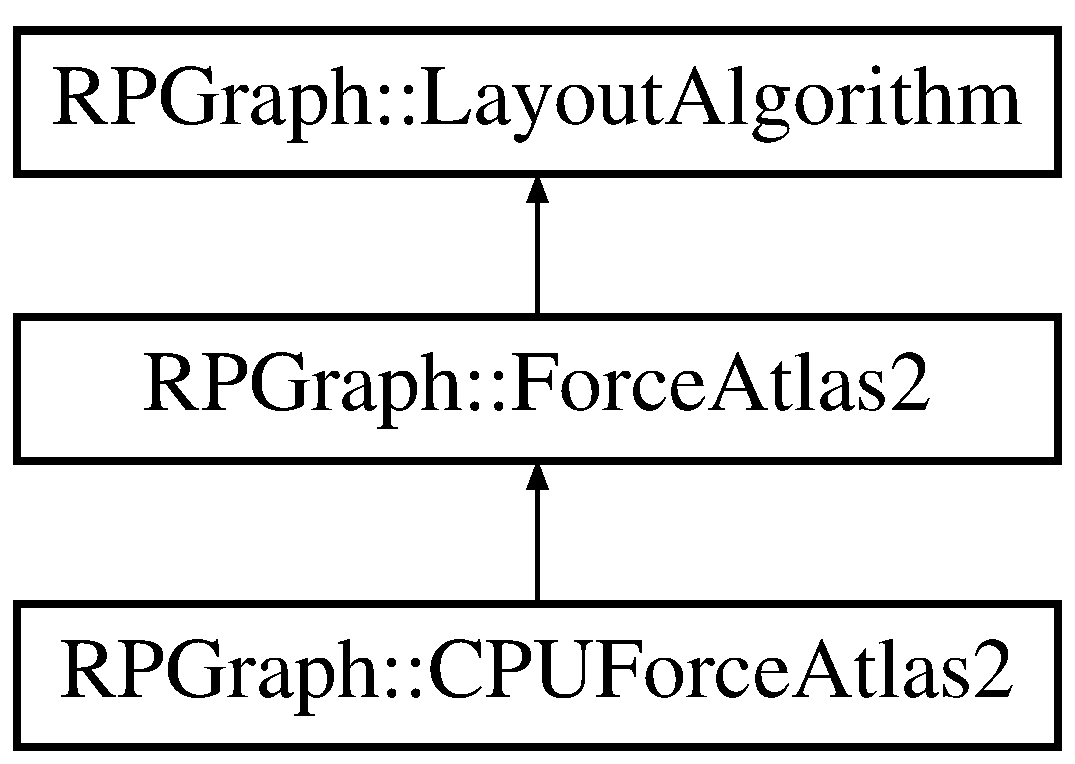
\includegraphics[height=3.000000cm]{classRPGraph_1_1CPUForceAtlas2}
\end{center}
\end{figure}
\subsection*{Public Member Functions}
\begin{DoxyCompactItemize}
\item 
\mbox{\hyperlink{classRPGraph_1_1CPUForceAtlas2_a5a17745426c0fcce430541f5b639282e}{C\+P\+U\+Force\+Atlas2}} (\mbox{\hyperlink{classRPGraph_1_1GraphLayout}{Graph\+Layout}} \&\mbox{\hyperlink{classRPGraph_1_1LayoutAlgorithm_ac2335a7ccaeb6cef789ea59b99353cf9}{layout}}, bool \mbox{\hyperlink{classRPGraph_1_1ForceAtlas2_a6ca74377ba79a67e4d1660c61426c090}{use\+\_\+barneshut}}, bool \mbox{\hyperlink{classRPGraph_1_1ForceAtlas2_afabfd0d83e05a54de889a62d0ff7595e}{strong\+\_\+gravity}}, float gravity, float scale)
\item 
\mbox{\hyperlink{classRPGraph_1_1CPUForceAtlas2_a0ea154bc6d1cca1dc47e4eda2152e0fe}{$\sim$\+C\+P\+U\+Force\+Atlas2}} ()
\item 
void \mbox{\hyperlink{classRPGraph_1_1CPUForceAtlas2_a3542ecd2220173aabe4e864fc21826eb}{do\+Step}} () override
\item 
void \mbox{\hyperlink{classRPGraph_1_1CPUForceAtlas2_afaada68053fce521843af0eb5ca316df}{sync\+\_\+layout}} () override
\end{DoxyCompactItemize}
\subsection*{Additional Inherited Members}


\subsection{Constructor \& Destructor Documentation}
\mbox{\Hypertarget{classRPGraph_1_1CPUForceAtlas2_a5a17745426c0fcce430541f5b639282e}\label{classRPGraph_1_1CPUForceAtlas2_a5a17745426c0fcce430541f5b639282e}} 
\index{R\+P\+Graph\+::\+C\+P\+U\+Force\+Atlas2@{R\+P\+Graph\+::\+C\+P\+U\+Force\+Atlas2}!C\+P\+U\+Force\+Atlas2@{C\+P\+U\+Force\+Atlas2}}
\index{C\+P\+U\+Force\+Atlas2@{C\+P\+U\+Force\+Atlas2}!R\+P\+Graph\+::\+C\+P\+U\+Force\+Atlas2@{R\+P\+Graph\+::\+C\+P\+U\+Force\+Atlas2}}
\subsubsection{\texorpdfstring{C\+P\+U\+Force\+Atlas2()}{CPUForceAtlas2()}}
{\footnotesize\ttfamily R\+P\+Graph\+::\+C\+P\+U\+Force\+Atlas2\+::\+C\+P\+U\+Force\+Atlas2 (\begin{DoxyParamCaption}\item[{\mbox{\hyperlink{classRPGraph_1_1GraphLayout}{Graph\+Layout}} \&}]{layout,  }\item[{bool}]{use\+\_\+barneshut,  }\item[{bool}]{strong\+\_\+gravity,  }\item[{float}]{gravity,  }\item[{float}]{scale }\end{DoxyParamCaption})}

\mbox{\Hypertarget{classRPGraph_1_1CPUForceAtlas2_a0ea154bc6d1cca1dc47e4eda2152e0fe}\label{classRPGraph_1_1CPUForceAtlas2_a0ea154bc6d1cca1dc47e4eda2152e0fe}} 
\index{R\+P\+Graph\+::\+C\+P\+U\+Force\+Atlas2@{R\+P\+Graph\+::\+C\+P\+U\+Force\+Atlas2}!````~C\+P\+U\+Force\+Atlas2@{$\sim$\+C\+P\+U\+Force\+Atlas2}}
\index{````~C\+P\+U\+Force\+Atlas2@{$\sim$\+C\+P\+U\+Force\+Atlas2}!R\+P\+Graph\+::\+C\+P\+U\+Force\+Atlas2@{R\+P\+Graph\+::\+C\+P\+U\+Force\+Atlas2}}
\subsubsection{\texorpdfstring{$\sim$\+C\+P\+U\+Force\+Atlas2()}{~CPUForceAtlas2()}}
{\footnotesize\ttfamily R\+P\+Graph\+::\+C\+P\+U\+Force\+Atlas2\+::$\sim$\+C\+P\+U\+Force\+Atlas2 (\begin{DoxyParamCaption}{ }\end{DoxyParamCaption})}



\subsection{Member Function Documentation}
\mbox{\Hypertarget{classRPGraph_1_1CPUForceAtlas2_a3542ecd2220173aabe4e864fc21826eb}\label{classRPGraph_1_1CPUForceAtlas2_a3542ecd2220173aabe4e864fc21826eb}} 
\index{R\+P\+Graph\+::\+C\+P\+U\+Force\+Atlas2@{R\+P\+Graph\+::\+C\+P\+U\+Force\+Atlas2}!do\+Step@{do\+Step}}
\index{do\+Step@{do\+Step}!R\+P\+Graph\+::\+C\+P\+U\+Force\+Atlas2@{R\+P\+Graph\+::\+C\+P\+U\+Force\+Atlas2}}
\subsubsection{\texorpdfstring{do\+Step()}{doStep()}}
{\footnotesize\ttfamily void R\+P\+Graph\+::\+C\+P\+U\+Force\+Atlas2\+::do\+Step (\begin{DoxyParamCaption}{ }\end{DoxyParamCaption})\hspace{0.3cm}{\ttfamily [override]}, {\ttfamily [virtual]}}

The tip of the spear. 

Implements \mbox{\hyperlink{classRPGraph_1_1ForceAtlas2_aa448ceec8292797a6e1b61ef8e2b3744}{R\+P\+Graph\+::\+Force\+Atlas2}}.

\mbox{\Hypertarget{classRPGraph_1_1CPUForceAtlas2_afaada68053fce521843af0eb5ca316df}\label{classRPGraph_1_1CPUForceAtlas2_afaada68053fce521843af0eb5ca316df}} 
\index{R\+P\+Graph\+::\+C\+P\+U\+Force\+Atlas2@{R\+P\+Graph\+::\+C\+P\+U\+Force\+Atlas2}!sync\+\_\+layout@{sync\+\_\+layout}}
\index{sync\+\_\+layout@{sync\+\_\+layout}!R\+P\+Graph\+::\+C\+P\+U\+Force\+Atlas2@{R\+P\+Graph\+::\+C\+P\+U\+Force\+Atlas2}}
\subsubsection{\texorpdfstring{sync\+\_\+layout()}{sync\_layout()}}
{\footnotesize\ttfamily void R\+P\+Graph\+::\+C\+P\+U\+Force\+Atlas2\+::sync\+\_\+layout (\begin{DoxyParamCaption}{ }\end{DoxyParamCaption})\hspace{0.3cm}{\ttfamily [override]}, {\ttfamily [virtual]}}



Implements \mbox{\hyperlink{classRPGraph_1_1LayoutAlgorithm_a70f3171d513b92d44f4784ff96c848c1}{R\+P\+Graph\+::\+Layout\+Algorithm}}.



The documentation for this class was generated from the following files\+:\begin{DoxyCompactItemize}
\item 
\mbox{\hyperlink{RPCPUForceAtlas2_8hpp}{R\+P\+C\+P\+U\+Force\+Atlas2.\+hpp}}\item 
\mbox{\hyperlink{RPCPUForceAtlas2_8cpp}{R\+P\+C\+P\+U\+Force\+Atlas2.\+cpp}}\end{DoxyCompactItemize}

\hypertarget{classRPGraph_1_1CSRUGraph}{}\section{R\+P\+Graph\+:\+:C\+S\+R\+U\+Graph Class Reference}
\label{classRPGraph_1_1CSRUGraph}\index{R\+P\+Graph\+::\+C\+S\+R\+U\+Graph@{R\+P\+Graph\+::\+C\+S\+R\+U\+Graph}}


{\ttfamily \#include $<$R\+P\+Graph.\+hpp$>$}

Inheritance diagram for R\+P\+Graph\+:\+:C\+S\+R\+U\+Graph\+:\begin{figure}[H]
\begin{center}
\leavevmode
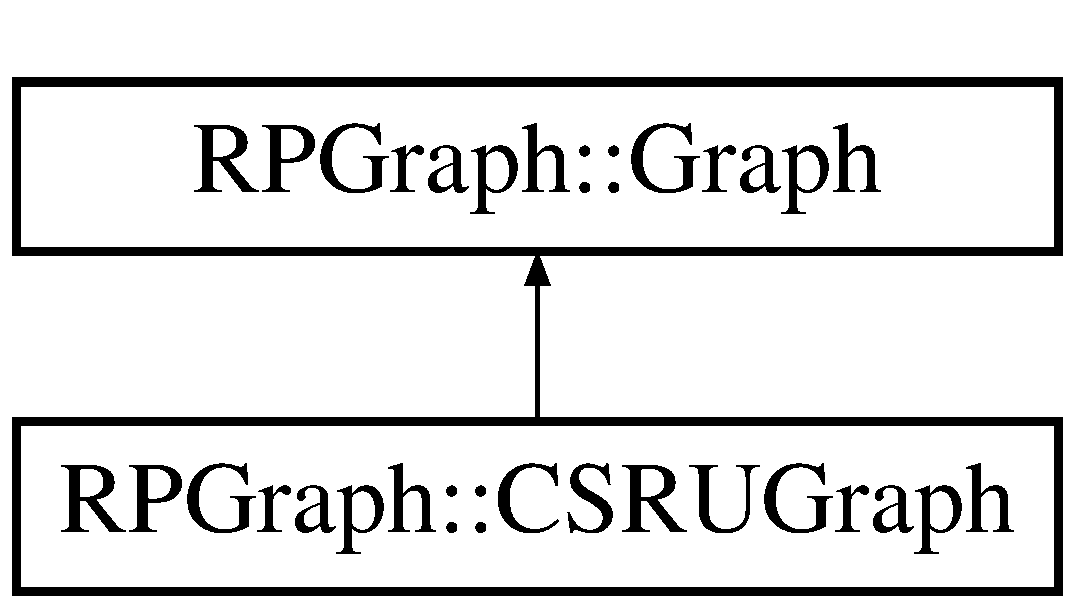
\includegraphics[height=2.000000cm]{classRPGraph_1_1CSRUGraph}
\end{center}
\end{figure}
\subsection*{Public Member Functions}
\begin{DoxyCompactItemize}
\item 
\mbox{\hyperlink{classRPGraph_1_1CSRUGraph_a78cc1f4446190dcd347edc6bfaa4c1b8}{C\+S\+R\+U\+Graph}} (\mbox{\hyperlink{namespaceRPGraph_ab3ae34f1ab88e48f43794c30c8697b74}{nid\+\_\+t}} \mbox{\hyperlink{classRPGraph_1_1CSRUGraph_a715af46d35bbe09b6b7d724461a1c2a5}{num\+\_\+nodes}}, \mbox{\hyperlink{namespaceRPGraph_ab3ae34f1ab88e48f43794c30c8697b74}{nid\+\_\+t}} \mbox{\hyperlink{classRPGraph_1_1CSRUGraph_a90ef3e196b0e234c8806bc455031018d}{num\+\_\+edges}})
\item 
\mbox{\hyperlink{classRPGraph_1_1CSRUGraph_a3e6cc9a4ef614b841519df3ea5d3715b}{$\sim$\+C\+S\+R\+U\+Graph}} ()
\item 
void \mbox{\hyperlink{classRPGraph_1_1CSRUGraph_a8d9cba867ebb6116cb391b78ad7ae31e}{insert\+\_\+node}} (\mbox{\hyperlink{namespaceRPGraph_ab3ae34f1ab88e48f43794c30c8697b74}{nid\+\_\+t}} node\+\_\+id, std\+::vector$<$ \mbox{\hyperlink{namespaceRPGraph_ab3ae34f1ab88e48f43794c30c8697b74}{nid\+\_\+t}} $>$ nbr\+\_\+ids)
\item 
void \mbox{\hyperlink{classRPGraph_1_1CSRUGraph_a5394625002cf95dbeac709f230d9f618}{fix\+\_\+edge\+\_\+ids}} ()
\item 
virtual \mbox{\hyperlink{namespaceRPGraph_ab3ae34f1ab88e48f43794c30c8697b74}{nid\+\_\+t}} \mbox{\hyperlink{classRPGraph_1_1CSRUGraph_a715af46d35bbe09b6b7d724461a1c2a5}{num\+\_\+nodes}} () override
\item 
virtual \mbox{\hyperlink{namespaceRPGraph_ab3ae34f1ab88e48f43794c30c8697b74}{nid\+\_\+t}} \mbox{\hyperlink{classRPGraph_1_1CSRUGraph_a90ef3e196b0e234c8806bc455031018d}{num\+\_\+edges}} () override
\item 
virtual \mbox{\hyperlink{namespaceRPGraph_ab3ae34f1ab88e48f43794c30c8697b74}{nid\+\_\+t}} \mbox{\hyperlink{classRPGraph_1_1CSRUGraph_ae2f3bb7a5ee2b53c88145a0cee6ed277}{degree}} (\mbox{\hyperlink{namespaceRPGraph_ab3ae34f1ab88e48f43794c30c8697b74}{nid\+\_\+t}} nid) override
\item 
virtual \mbox{\hyperlink{namespaceRPGraph_ab3ae34f1ab88e48f43794c30c8697b74}{nid\+\_\+t}} \mbox{\hyperlink{classRPGraph_1_1CSRUGraph_a88965d72f2fbea43b6d731d2cc027858}{in\+\_\+degree}} (\mbox{\hyperlink{namespaceRPGraph_ab3ae34f1ab88e48f43794c30c8697b74}{nid\+\_\+t}} nid) override
\item 
virtual \mbox{\hyperlink{namespaceRPGraph_ab3ae34f1ab88e48f43794c30c8697b74}{nid\+\_\+t}} \mbox{\hyperlink{classRPGraph_1_1CSRUGraph_a952e2a8eea28c0d879a0b5688d0e1b06}{out\+\_\+degree}} (\mbox{\hyperlink{namespaceRPGraph_ab3ae34f1ab88e48f43794c30c8697b74}{nid\+\_\+t}} nid) override
\item 
\mbox{\hyperlink{namespaceRPGraph_ab3ae34f1ab88e48f43794c30c8697b74}{nid\+\_\+t}} \mbox{\hyperlink{classRPGraph_1_1CSRUGraph_a17284d198dac4fb4611ffda71c679471}{nbr\+\_\+id\+\_\+for\+\_\+node}} (\mbox{\hyperlink{namespaceRPGraph_ab3ae34f1ab88e48f43794c30c8697b74}{nid\+\_\+t}} nid, \mbox{\hyperlink{namespaceRPGraph_ab3ae34f1ab88e48f43794c30c8697b74}{nid\+\_\+t}} nbr\+\_\+no)
\end{DoxyCompactItemize}
\subsection*{Public Attributes}
\begin{DoxyCompactItemize}
\item 
std\+::unordered\+\_\+map$<$ \mbox{\hyperlink{namespaceRPGraph_ab3ae34f1ab88e48f43794c30c8697b74}{nid\+\_\+t}}, \mbox{\hyperlink{namespaceRPGraph_ab3ae34f1ab88e48f43794c30c8697b74}{nid\+\_\+t}} $>$ \mbox{\hyperlink{classRPGraph_1_1CSRUGraph_a4d831eac19d0c676ff02e542250d429c}{nid\+\_\+to\+\_\+offset}}
\item 
\mbox{\hyperlink{namespaceRPGraph_ab3ae34f1ab88e48f43794c30c8697b74}{nid\+\_\+t}} $\ast$ \mbox{\hyperlink{classRPGraph_1_1CSRUGraph_ad59e162f4c9eeac87a0fbd5d3c054dbe}{offset\+\_\+to\+\_\+nid}}
\end{DoxyCompactItemize}


\subsection{Constructor \& Destructor Documentation}
\mbox{\Hypertarget{classRPGraph_1_1CSRUGraph_a78cc1f4446190dcd347edc6bfaa4c1b8}\label{classRPGraph_1_1CSRUGraph_a78cc1f4446190dcd347edc6bfaa4c1b8}} 
\index{R\+P\+Graph\+::\+C\+S\+R\+U\+Graph@{R\+P\+Graph\+::\+C\+S\+R\+U\+Graph}!C\+S\+R\+U\+Graph@{C\+S\+R\+U\+Graph}}
\index{C\+S\+R\+U\+Graph@{C\+S\+R\+U\+Graph}!R\+P\+Graph\+::\+C\+S\+R\+U\+Graph@{R\+P\+Graph\+::\+C\+S\+R\+U\+Graph}}
\subsubsection{\texorpdfstring{C\+S\+R\+U\+Graph()}{CSRUGraph()}}
{\footnotesize\ttfamily R\+P\+Graph\+::\+C\+S\+R\+U\+Graph\+::\+C\+S\+R\+U\+Graph (\begin{DoxyParamCaption}\item[{\mbox{\hyperlink{namespaceRPGraph_ab3ae34f1ab88e48f43794c30c8697b74}{nid\+\_\+t}}}]{num\+\_\+nodes,  }\item[{\mbox{\hyperlink{namespaceRPGraph_ab3ae34f1ab88e48f43794c30c8697b74}{nid\+\_\+t}}}]{num\+\_\+edges }\end{DoxyParamCaption})}

I\+M\+P\+O\+R\+T\+A\+NT\+: Ignore this data structure. Not used in implementation. \mbox{\Hypertarget{classRPGraph_1_1CSRUGraph_a3e6cc9a4ef614b841519df3ea5d3715b}\label{classRPGraph_1_1CSRUGraph_a3e6cc9a4ef614b841519df3ea5d3715b}} 
\index{R\+P\+Graph\+::\+C\+S\+R\+U\+Graph@{R\+P\+Graph\+::\+C\+S\+R\+U\+Graph}!````~C\+S\+R\+U\+Graph@{$\sim$\+C\+S\+R\+U\+Graph}}
\index{````~C\+S\+R\+U\+Graph@{$\sim$\+C\+S\+R\+U\+Graph}!R\+P\+Graph\+::\+C\+S\+R\+U\+Graph@{R\+P\+Graph\+::\+C\+S\+R\+U\+Graph}}
\subsubsection{\texorpdfstring{$\sim$\+C\+S\+R\+U\+Graph()}{~CSRUGraph()}}
{\footnotesize\ttfamily R\+P\+Graph\+::\+C\+S\+R\+U\+Graph\+::$\sim$\+C\+S\+R\+U\+Graph (\begin{DoxyParamCaption}{ }\end{DoxyParamCaption})}



\subsection{Member Function Documentation}
\mbox{\Hypertarget{classRPGraph_1_1CSRUGraph_ae2f3bb7a5ee2b53c88145a0cee6ed277}\label{classRPGraph_1_1CSRUGraph_ae2f3bb7a5ee2b53c88145a0cee6ed277}} 
\index{R\+P\+Graph\+::\+C\+S\+R\+U\+Graph@{R\+P\+Graph\+::\+C\+S\+R\+U\+Graph}!degree@{degree}}
\index{degree@{degree}!R\+P\+Graph\+::\+C\+S\+R\+U\+Graph@{R\+P\+Graph\+::\+C\+S\+R\+U\+Graph}}
\subsubsection{\texorpdfstring{degree()}{degree()}}
{\footnotesize\ttfamily \mbox{\hyperlink{namespaceRPGraph_ab3ae34f1ab88e48f43794c30c8697b74}{nid\+\_\+t}} R\+P\+Graph\+::\+C\+S\+R\+U\+Graph\+::degree (\begin{DoxyParamCaption}\item[{\mbox{\hyperlink{namespaceRPGraph_ab3ae34f1ab88e48f43794c30c8697b74}{nid\+\_\+t}}}]{nid }\end{DoxyParamCaption})\hspace{0.3cm}{\ttfamily [override]}, {\ttfamily [virtual]}}



Implements \mbox{\hyperlink{classRPGraph_1_1Graph_a8a95d1f403c3d9860cf7399abc820c7d}{R\+P\+Graph\+::\+Graph}}.

\mbox{\Hypertarget{classRPGraph_1_1CSRUGraph_a5394625002cf95dbeac709f230d9f618}\label{classRPGraph_1_1CSRUGraph_a5394625002cf95dbeac709f230d9f618}} 
\index{R\+P\+Graph\+::\+C\+S\+R\+U\+Graph@{R\+P\+Graph\+::\+C\+S\+R\+U\+Graph}!fix\+\_\+edge\+\_\+ids@{fix\+\_\+edge\+\_\+ids}}
\index{fix\+\_\+edge\+\_\+ids@{fix\+\_\+edge\+\_\+ids}!R\+P\+Graph\+::\+C\+S\+R\+U\+Graph@{R\+P\+Graph\+::\+C\+S\+R\+U\+Graph}}
\subsubsection{\texorpdfstring{fix\+\_\+edge\+\_\+ids()}{fix\_edge\_ids()}}
{\footnotesize\ttfamily void R\+P\+Graph\+::\+C\+S\+R\+U\+Graph\+::fix\+\_\+edge\+\_\+ids (\begin{DoxyParamCaption}{ }\end{DoxyParamCaption})}

\mbox{\Hypertarget{classRPGraph_1_1CSRUGraph_a88965d72f2fbea43b6d731d2cc027858}\label{classRPGraph_1_1CSRUGraph_a88965d72f2fbea43b6d731d2cc027858}} 
\index{R\+P\+Graph\+::\+C\+S\+R\+U\+Graph@{R\+P\+Graph\+::\+C\+S\+R\+U\+Graph}!in\+\_\+degree@{in\+\_\+degree}}
\index{in\+\_\+degree@{in\+\_\+degree}!R\+P\+Graph\+::\+C\+S\+R\+U\+Graph@{R\+P\+Graph\+::\+C\+S\+R\+U\+Graph}}
\subsubsection{\texorpdfstring{in\+\_\+degree()}{in\_degree()}}
{\footnotesize\ttfamily \mbox{\hyperlink{namespaceRPGraph_ab3ae34f1ab88e48f43794c30c8697b74}{nid\+\_\+t}} R\+P\+Graph\+::\+C\+S\+R\+U\+Graph\+::in\+\_\+degree (\begin{DoxyParamCaption}\item[{\mbox{\hyperlink{namespaceRPGraph_ab3ae34f1ab88e48f43794c30c8697b74}{nid\+\_\+t}}}]{nid }\end{DoxyParamCaption})\hspace{0.3cm}{\ttfamily [override]}, {\ttfamily [virtual]}}



Implements \mbox{\hyperlink{classRPGraph_1_1Graph_ab75e19f698a4ab99e37593c7178f2c1a}{R\+P\+Graph\+::\+Graph}}.

\mbox{\Hypertarget{classRPGraph_1_1CSRUGraph_a8d9cba867ebb6116cb391b78ad7ae31e}\label{classRPGraph_1_1CSRUGraph_a8d9cba867ebb6116cb391b78ad7ae31e}} 
\index{R\+P\+Graph\+::\+C\+S\+R\+U\+Graph@{R\+P\+Graph\+::\+C\+S\+R\+U\+Graph}!insert\+\_\+node@{insert\+\_\+node}}
\index{insert\+\_\+node@{insert\+\_\+node}!R\+P\+Graph\+::\+C\+S\+R\+U\+Graph@{R\+P\+Graph\+::\+C\+S\+R\+U\+Graph}}
\subsubsection{\texorpdfstring{insert\+\_\+node()}{insert\_node()}}
{\footnotesize\ttfamily void R\+P\+Graph\+::\+C\+S\+R\+U\+Graph\+::insert\+\_\+node (\begin{DoxyParamCaption}\item[{\mbox{\hyperlink{namespaceRPGraph_ab3ae34f1ab88e48f43794c30c8697b74}{nid\+\_\+t}}}]{node\+\_\+id,  }\item[{std\+::vector$<$ \mbox{\hyperlink{namespaceRPGraph_ab3ae34f1ab88e48f43794c30c8697b74}{nid\+\_\+t}} $>$}]{nbr\+\_\+ids }\end{DoxyParamCaption})}

Inserts node\+\_\+id and its edges. Once inserted, edges can\textquotesingle{}t be altered for this node. \mbox{\Hypertarget{classRPGraph_1_1CSRUGraph_a17284d198dac4fb4611ffda71c679471}\label{classRPGraph_1_1CSRUGraph_a17284d198dac4fb4611ffda71c679471}} 
\index{R\+P\+Graph\+::\+C\+S\+R\+U\+Graph@{R\+P\+Graph\+::\+C\+S\+R\+U\+Graph}!nbr\+\_\+id\+\_\+for\+\_\+node@{nbr\+\_\+id\+\_\+for\+\_\+node}}
\index{nbr\+\_\+id\+\_\+for\+\_\+node@{nbr\+\_\+id\+\_\+for\+\_\+node}!R\+P\+Graph\+::\+C\+S\+R\+U\+Graph@{R\+P\+Graph\+::\+C\+S\+R\+U\+Graph}}
\subsubsection{\texorpdfstring{nbr\+\_\+id\+\_\+for\+\_\+node()}{nbr\_id\_for\_node()}}
{\footnotesize\ttfamily \mbox{\hyperlink{namespaceRPGraph_ab3ae34f1ab88e48f43794c30c8697b74}{nid\+\_\+t}} R\+P\+Graph\+::\+C\+S\+R\+U\+Graph\+::nbr\+\_\+id\+\_\+for\+\_\+node (\begin{DoxyParamCaption}\item[{\mbox{\hyperlink{namespaceRPGraph_ab3ae34f1ab88e48f43794c30c8697b74}{nid\+\_\+t}}}]{nid,  }\item[{\mbox{\hyperlink{namespaceRPGraph_ab3ae34f1ab88e48f43794c30c8697b74}{nid\+\_\+t}}}]{nbr\+\_\+no }\end{DoxyParamCaption})}

\mbox{\Hypertarget{classRPGraph_1_1CSRUGraph_a90ef3e196b0e234c8806bc455031018d}\label{classRPGraph_1_1CSRUGraph_a90ef3e196b0e234c8806bc455031018d}} 
\index{R\+P\+Graph\+::\+C\+S\+R\+U\+Graph@{R\+P\+Graph\+::\+C\+S\+R\+U\+Graph}!num\+\_\+edges@{num\+\_\+edges}}
\index{num\+\_\+edges@{num\+\_\+edges}!R\+P\+Graph\+::\+C\+S\+R\+U\+Graph@{R\+P\+Graph\+::\+C\+S\+R\+U\+Graph}}
\subsubsection{\texorpdfstring{num\+\_\+edges()}{num\_edges()}}
{\footnotesize\ttfamily \mbox{\hyperlink{namespaceRPGraph_ab3ae34f1ab88e48f43794c30c8697b74}{nid\+\_\+t}} R\+P\+Graph\+::\+C\+S\+R\+U\+Graph\+::num\+\_\+edges (\begin{DoxyParamCaption}{ }\end{DoxyParamCaption})\hspace{0.3cm}{\ttfamily [override]}, {\ttfamily [virtual]}}



Implements \mbox{\hyperlink{classRPGraph_1_1Graph_acd3b877216686aff2f7fbc2d62bcdf9b}{R\+P\+Graph\+::\+Graph}}.

\mbox{\Hypertarget{classRPGraph_1_1CSRUGraph_a715af46d35bbe09b6b7d724461a1c2a5}\label{classRPGraph_1_1CSRUGraph_a715af46d35bbe09b6b7d724461a1c2a5}} 
\index{R\+P\+Graph\+::\+C\+S\+R\+U\+Graph@{R\+P\+Graph\+::\+C\+S\+R\+U\+Graph}!num\+\_\+nodes@{num\+\_\+nodes}}
\index{num\+\_\+nodes@{num\+\_\+nodes}!R\+P\+Graph\+::\+C\+S\+R\+U\+Graph@{R\+P\+Graph\+::\+C\+S\+R\+U\+Graph}}
\subsubsection{\texorpdfstring{num\+\_\+nodes()}{num\_nodes()}}
{\footnotesize\ttfamily \mbox{\hyperlink{namespaceRPGraph_ab3ae34f1ab88e48f43794c30c8697b74}{nid\+\_\+t}} R\+P\+Graph\+::\+C\+S\+R\+U\+Graph\+::num\+\_\+nodes (\begin{DoxyParamCaption}{ }\end{DoxyParamCaption})\hspace{0.3cm}{\ttfamily [override]}, {\ttfamily [virtual]}}



Implements \mbox{\hyperlink{classRPGraph_1_1Graph_ab5602e6b776a0ea3b944775331fcb2aa}{R\+P\+Graph\+::\+Graph}}.

\mbox{\Hypertarget{classRPGraph_1_1CSRUGraph_a952e2a8eea28c0d879a0b5688d0e1b06}\label{classRPGraph_1_1CSRUGraph_a952e2a8eea28c0d879a0b5688d0e1b06}} 
\index{R\+P\+Graph\+::\+C\+S\+R\+U\+Graph@{R\+P\+Graph\+::\+C\+S\+R\+U\+Graph}!out\+\_\+degree@{out\+\_\+degree}}
\index{out\+\_\+degree@{out\+\_\+degree}!R\+P\+Graph\+::\+C\+S\+R\+U\+Graph@{R\+P\+Graph\+::\+C\+S\+R\+U\+Graph}}
\subsubsection{\texorpdfstring{out\+\_\+degree()}{out\_degree()}}
{\footnotesize\ttfamily \mbox{\hyperlink{namespaceRPGraph_ab3ae34f1ab88e48f43794c30c8697b74}{nid\+\_\+t}} R\+P\+Graph\+::\+C\+S\+R\+U\+Graph\+::out\+\_\+degree (\begin{DoxyParamCaption}\item[{\mbox{\hyperlink{namespaceRPGraph_ab3ae34f1ab88e48f43794c30c8697b74}{nid\+\_\+t}}}]{nid }\end{DoxyParamCaption})\hspace{0.3cm}{\ttfamily [override]}, {\ttfamily [virtual]}}



Implements \mbox{\hyperlink{classRPGraph_1_1Graph_a660ad58e03df7e3cc00d0eb4e5c16819}{R\+P\+Graph\+::\+Graph}}.



\subsection{Member Data Documentation}
\mbox{\Hypertarget{classRPGraph_1_1CSRUGraph_a4d831eac19d0c676ff02e542250d429c}\label{classRPGraph_1_1CSRUGraph_a4d831eac19d0c676ff02e542250d429c}} 
\index{R\+P\+Graph\+::\+C\+S\+R\+U\+Graph@{R\+P\+Graph\+::\+C\+S\+R\+U\+Graph}!nid\+\_\+to\+\_\+offset@{nid\+\_\+to\+\_\+offset}}
\index{nid\+\_\+to\+\_\+offset@{nid\+\_\+to\+\_\+offset}!R\+P\+Graph\+::\+C\+S\+R\+U\+Graph@{R\+P\+Graph\+::\+C\+S\+R\+U\+Graph}}
\subsubsection{\texorpdfstring{nid\+\_\+to\+\_\+offset}{nid\_to\_offset}}
{\footnotesize\ttfamily std\+::unordered\+\_\+map$<$\mbox{\hyperlink{namespaceRPGraph_ab3ae34f1ab88e48f43794c30c8697b74}{nid\+\_\+t}}, \mbox{\hyperlink{namespaceRPGraph_ab3ae34f1ab88e48f43794c30c8697b74}{nid\+\_\+t}}$>$ R\+P\+Graph\+::\+C\+S\+R\+U\+Graph\+::nid\+\_\+to\+\_\+offset}

\mbox{\Hypertarget{classRPGraph_1_1CSRUGraph_ad59e162f4c9eeac87a0fbd5d3c054dbe}\label{classRPGraph_1_1CSRUGraph_ad59e162f4c9eeac87a0fbd5d3c054dbe}} 
\index{R\+P\+Graph\+::\+C\+S\+R\+U\+Graph@{R\+P\+Graph\+::\+C\+S\+R\+U\+Graph}!offset\+\_\+to\+\_\+nid@{offset\+\_\+to\+\_\+nid}}
\index{offset\+\_\+to\+\_\+nid@{offset\+\_\+to\+\_\+nid}!R\+P\+Graph\+::\+C\+S\+R\+U\+Graph@{R\+P\+Graph\+::\+C\+S\+R\+U\+Graph}}
\subsubsection{\texorpdfstring{offset\+\_\+to\+\_\+nid}{offset\_to\_nid}}
{\footnotesize\ttfamily \mbox{\hyperlink{namespaceRPGraph_ab3ae34f1ab88e48f43794c30c8697b74}{nid\+\_\+t}}$\ast$ R\+P\+Graph\+::\+C\+S\+R\+U\+Graph\+::offset\+\_\+to\+\_\+nid}



The documentation for this class was generated from the following files\+:\begin{DoxyCompactItemize}
\item 
\mbox{\hyperlink{RPGraph_8hpp}{R\+P\+Graph.\+hpp}}\item 
\mbox{\hyperlink{RPGraph_8cpp}{R\+P\+Graph.\+cpp}}\end{DoxyCompactItemize}

\hypertarget{classRPGraph_1_1CUDAForceAtlas2}{}\section{R\+P\+Graph\+:\+:C\+U\+D\+A\+Force\+Atlas2 Class Reference}
\label{classRPGraph_1_1CUDAForceAtlas2}\index{R\+P\+Graph\+::\+C\+U\+D\+A\+Force\+Atlas2@{R\+P\+Graph\+::\+C\+U\+D\+A\+Force\+Atlas2}}


{\ttfamily \#include $<$R\+P\+G\+P\+U\+Force\+Atlas2.\+hpp$>$}

Inheritance diagram for R\+P\+Graph\+:\+:C\+U\+D\+A\+Force\+Atlas2\+:\begin{figure}[H]
\begin{center}
\leavevmode
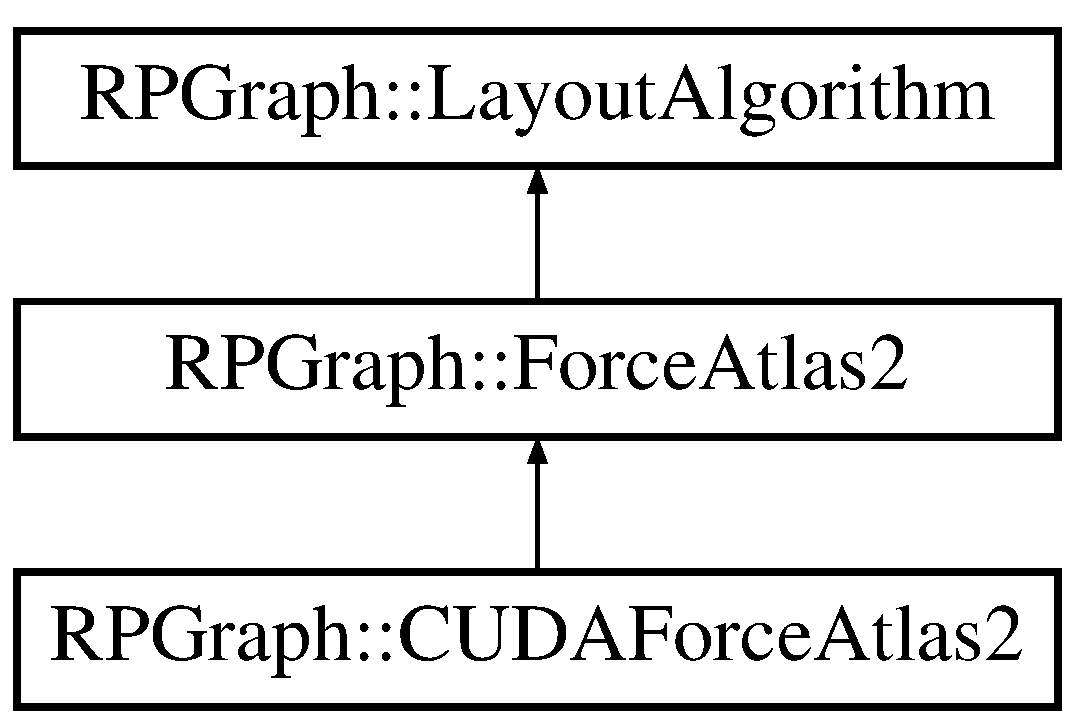
\includegraphics[height=3.000000cm]{classRPGraph_1_1CUDAForceAtlas2}
\end{center}
\end{figure}
\subsection*{Public Member Functions}
\begin{DoxyCompactItemize}
\item 
\mbox{\hyperlink{classRPGraph_1_1CUDAForceAtlas2_a8cdd430ec7758697fe362cfbca2fd311}{C\+U\+D\+A\+Force\+Atlas2}} (\mbox{\hyperlink{classRPGraph_1_1GraphLayout}{Graph\+Layout}} \&\mbox{\hyperlink{classRPGraph_1_1LayoutAlgorithm_ac2335a7ccaeb6cef789ea59b99353cf9}{layout}}, bool \mbox{\hyperlink{classRPGraph_1_1ForceAtlas2_a6ca74377ba79a67e4d1660c61426c090}{use\+\_\+barneshut}}, bool \mbox{\hyperlink{classRPGraph_1_1ForceAtlas2_afabfd0d83e05a54de889a62d0ff7595e}{strong\+\_\+gravity}}, float gravity, float scale)
\item 
\mbox{\hyperlink{classRPGraph_1_1CUDAForceAtlas2_a5a57cb10f336ced8b717dbfa16cc4051}{$\sim$\+C\+U\+D\+A\+Force\+Atlas2}} ()
\item 
void \mbox{\hyperlink{classRPGraph_1_1CUDAForceAtlas2_a4ebfb858b5c2c19b9e57ef1d434a21a7}{do\+Step}} () override
\item 
void \mbox{\hyperlink{classRPGraph_1_1CUDAForceAtlas2_a474a1cd717352057859185885b8020cf}{sync\+\_\+layout}} () override
\end{DoxyCompactItemize}
\subsection*{Additional Inherited Members}


\subsection{Constructor \& Destructor Documentation}
\mbox{\Hypertarget{classRPGraph_1_1CUDAForceAtlas2_a8cdd430ec7758697fe362cfbca2fd311}\label{classRPGraph_1_1CUDAForceAtlas2_a8cdd430ec7758697fe362cfbca2fd311}} 
\index{R\+P\+Graph\+::\+C\+U\+D\+A\+Force\+Atlas2@{R\+P\+Graph\+::\+C\+U\+D\+A\+Force\+Atlas2}!C\+U\+D\+A\+Force\+Atlas2@{C\+U\+D\+A\+Force\+Atlas2}}
\index{C\+U\+D\+A\+Force\+Atlas2@{C\+U\+D\+A\+Force\+Atlas2}!R\+P\+Graph\+::\+C\+U\+D\+A\+Force\+Atlas2@{R\+P\+Graph\+::\+C\+U\+D\+A\+Force\+Atlas2}}
\subsubsection{\texorpdfstring{C\+U\+D\+A\+Force\+Atlas2()}{CUDAForceAtlas2()}}
{\footnotesize\ttfamily R\+P\+Graph\+::\+C\+U\+D\+A\+Force\+Atlas2\+::\+C\+U\+D\+A\+Force\+Atlas2 (\begin{DoxyParamCaption}\item[{\mbox{\hyperlink{classRPGraph_1_1GraphLayout}{Graph\+Layout}} \&}]{layout,  }\item[{bool}]{use\+\_\+barneshut,  }\item[{bool}]{strong\+\_\+gravity,  }\item[{float}]{gravity,  }\item[{float}]{scale }\end{DoxyParamCaption})}

\mbox{\Hypertarget{classRPGraph_1_1CUDAForceAtlas2_a5a57cb10f336ced8b717dbfa16cc4051}\label{classRPGraph_1_1CUDAForceAtlas2_a5a57cb10f336ced8b717dbfa16cc4051}} 
\index{R\+P\+Graph\+::\+C\+U\+D\+A\+Force\+Atlas2@{R\+P\+Graph\+::\+C\+U\+D\+A\+Force\+Atlas2}!````~C\+U\+D\+A\+Force\+Atlas2@{$\sim$\+C\+U\+D\+A\+Force\+Atlas2}}
\index{````~C\+U\+D\+A\+Force\+Atlas2@{$\sim$\+C\+U\+D\+A\+Force\+Atlas2}!R\+P\+Graph\+::\+C\+U\+D\+A\+Force\+Atlas2@{R\+P\+Graph\+::\+C\+U\+D\+A\+Force\+Atlas2}}
\subsubsection{\texorpdfstring{$\sim$\+C\+U\+D\+A\+Force\+Atlas2()}{~CUDAForceAtlas2()}}
{\footnotesize\ttfamily R\+P\+Graph\+::\+C\+U\+D\+A\+Force\+Atlas2\+::$\sim$\+C\+U\+D\+A\+Force\+Atlas2 (\begin{DoxyParamCaption}{ }\end{DoxyParamCaption})}



\subsection{Member Function Documentation}
\mbox{\Hypertarget{classRPGraph_1_1CUDAForceAtlas2_a4ebfb858b5c2c19b9e57ef1d434a21a7}\label{classRPGraph_1_1CUDAForceAtlas2_a4ebfb858b5c2c19b9e57ef1d434a21a7}} 
\index{R\+P\+Graph\+::\+C\+U\+D\+A\+Force\+Atlas2@{R\+P\+Graph\+::\+C\+U\+D\+A\+Force\+Atlas2}!do\+Step@{do\+Step}}
\index{do\+Step@{do\+Step}!R\+P\+Graph\+::\+C\+U\+D\+A\+Force\+Atlas2@{R\+P\+Graph\+::\+C\+U\+D\+A\+Force\+Atlas2}}
\subsubsection{\texorpdfstring{do\+Step()}{doStep()}}
{\footnotesize\ttfamily void R\+P\+Graph\+::\+C\+U\+D\+A\+Force\+Atlas2\+::do\+Step (\begin{DoxyParamCaption}{ }\end{DoxyParamCaption})\hspace{0.3cm}{\ttfamily [override]}, {\ttfamily [virtual]}}



Implements \mbox{\hyperlink{classRPGraph_1_1ForceAtlas2_aa448ceec8292797a6e1b61ef8e2b3744}{R\+P\+Graph\+::\+Force\+Atlas2}}.

\mbox{\Hypertarget{classRPGraph_1_1CUDAForceAtlas2_a474a1cd717352057859185885b8020cf}\label{classRPGraph_1_1CUDAForceAtlas2_a474a1cd717352057859185885b8020cf}} 
\index{R\+P\+Graph\+::\+C\+U\+D\+A\+Force\+Atlas2@{R\+P\+Graph\+::\+C\+U\+D\+A\+Force\+Atlas2}!sync\+\_\+layout@{sync\+\_\+layout}}
\index{sync\+\_\+layout@{sync\+\_\+layout}!R\+P\+Graph\+::\+C\+U\+D\+A\+Force\+Atlas2@{R\+P\+Graph\+::\+C\+U\+D\+A\+Force\+Atlas2}}
\subsubsection{\texorpdfstring{sync\+\_\+layout()}{sync\_layout()}}
{\footnotesize\ttfamily void R\+P\+Graph\+::\+C\+U\+D\+A\+Force\+Atlas2\+::sync\+\_\+layout (\begin{DoxyParamCaption}{ }\end{DoxyParamCaption})\hspace{0.3cm}{\ttfamily [override]}, {\ttfamily [virtual]}}



Implements \mbox{\hyperlink{classRPGraph_1_1LayoutAlgorithm_a70f3171d513b92d44f4784ff96c848c1}{R\+P\+Graph\+::\+Layout\+Algorithm}}.



The documentation for this class was generated from the following file\+:\begin{DoxyCompactItemize}
\item 
\mbox{\hyperlink{RPGPUForceAtlas2_8hpp}{R\+P\+G\+P\+U\+Force\+Atlas2.\+hpp}}\end{DoxyCompactItemize}

\hypertarget{classRPGraph_1_1ForceAtlas2}{}\section{R\+P\+Graph\+:\+:Force\+Atlas2 Class Reference}
\label{classRPGraph_1_1ForceAtlas2}\index{R\+P\+Graph\+::\+Force\+Atlas2@{R\+P\+Graph\+::\+Force\+Atlas2}}


{\ttfamily \#include $<$R\+P\+Force\+Atlas2.\+hpp$>$}

Inheritance diagram for R\+P\+Graph\+:\+:Force\+Atlas2\+:\begin{figure}[H]
\begin{center}
\leavevmode
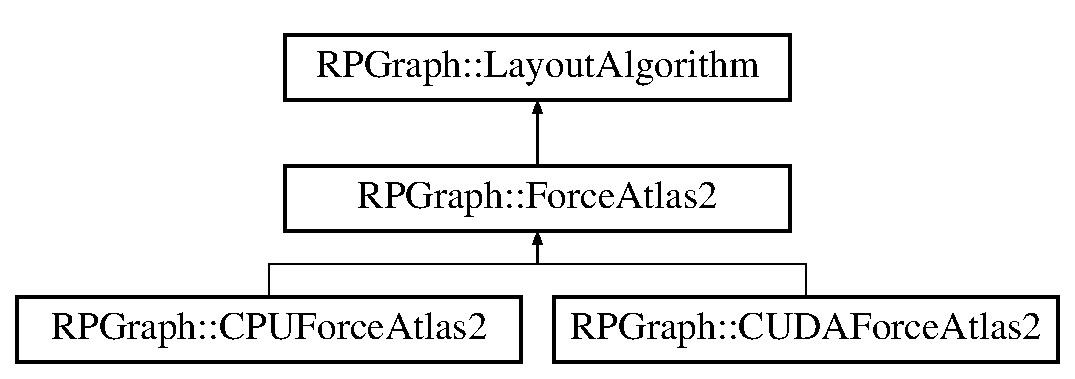
\includegraphics[height=3.000000cm]{classRPGraph_1_1ForceAtlas2}
\end{center}
\end{figure}
\subsection*{Public Member Functions}
\begin{DoxyCompactItemize}
\item 
\mbox{\hyperlink{classRPGraph_1_1ForceAtlas2_a4c7ce390cdedc886003571f31861eb0c}{Force\+Atlas2}} (\mbox{\hyperlink{classRPGraph_1_1GraphLayout}{Graph\+Layout}} \&\mbox{\hyperlink{classRPGraph_1_1LayoutAlgorithm_ac2335a7ccaeb6cef789ea59b99353cf9}{layout}}, bool \mbox{\hyperlink{classRPGraph_1_1ForceAtlas2_a6ca74377ba79a67e4d1660c61426c090}{use\+\_\+barneshut}}, bool \mbox{\hyperlink{classRPGraph_1_1ForceAtlas2_afabfd0d83e05a54de889a62d0ff7595e}{strong\+\_\+gravity}}, float gravity, float scale)
\item 
\mbox{\hyperlink{classRPGraph_1_1ForceAtlas2_a1be4cef4dacd90f3a6a7c3d216fd0e78}{$\sim$\+Force\+Atlas2}} ()
\item 
virtual void \mbox{\hyperlink{classRPGraph_1_1ForceAtlas2_aa448ceec8292797a6e1b61ef8e2b3744}{do\+Step}} ()=0
\item 
void \mbox{\hyperlink{classRPGraph_1_1ForceAtlas2_ae02d5fff5d824602da4885187361dfb5}{do\+Steps}} (int n)
\item 
void \mbox{\hyperlink{classRPGraph_1_1ForceAtlas2_af052a93a41b8de4d58a19cd142f09c43}{set\+Scale}} (float s)
\item 
void \mbox{\hyperlink{classRPGraph_1_1ForceAtlas2_a2648eec5e0e6c4ba524dec19be09bdfd}{set\+Gravity}} (float s)
\item 
float \mbox{\hyperlink{classRPGraph_1_1ForceAtlas2_ab08806505160d4a5ca2b746dd5a0b1c9}{mass}} (\mbox{\hyperlink{namespaceRPGraph_ab3ae34f1ab88e48f43794c30c8697b74}{nid\+\_\+t}} n)
\end{DoxyCompactItemize}
\subsection*{Public Attributes}
\begin{DoxyCompactItemize}
\item 
bool \mbox{\hyperlink{classRPGraph_1_1ForceAtlas2_ad2fa1a5b6042c22d44b84b85b10cffe1}{prevent\+\_\+overlap}}
\item 
bool \mbox{\hyperlink{classRPGraph_1_1ForceAtlas2_a6ca74377ba79a67e4d1660c61426c090}{use\+\_\+barneshut}}
\item 
bool \mbox{\hyperlink{classRPGraph_1_1ForceAtlas2_a5f1e78d982b10646f7d79fef5cc49ea7}{use\+\_\+linlog}}
\item 
bool \mbox{\hyperlink{classRPGraph_1_1ForceAtlas2_afabfd0d83e05a54de889a62d0ff7595e}{strong\+\_\+gravity}}
\end{DoxyCompactItemize}
\subsection*{Protected Attributes}
\begin{DoxyCompactItemize}
\item 
int \mbox{\hyperlink{classRPGraph_1_1ForceAtlas2_a3d382e3059747c692b1ef2b1cd49f44f}{iteration}}
\item 
float \mbox{\hyperlink{classRPGraph_1_1ForceAtlas2_ac0f82f64f66f1798d8f1ee5905ccf192}{k\+\_\+r}}
\item 
float \mbox{\hyperlink{classRPGraph_1_1ForceAtlas2_a4132cf261a746246639e0fb4960ba090}{k\+\_\+g}}
\item 
float \mbox{\hyperlink{classRPGraph_1_1ForceAtlas2_a39051fda34ae96395209e8b5657a61bd}{delta}}
\item 
float \mbox{\hyperlink{classRPGraph_1_1ForceAtlas2_a04219199074fb0c1df44ba407879931e}{global\+\_\+speed}}
\item 
float \mbox{\hyperlink{classRPGraph_1_1ForceAtlas2_aeb9cda3185f43eb86228ff94cbbfdc70}{speed\+\_\+efficiency}}
\item 
float \mbox{\hyperlink{classRPGraph_1_1ForceAtlas2_a8b16236d6e7ba96fd336a6ee42409cad}{jitter\+\_\+tolerance}}
\item 
float \mbox{\hyperlink{classRPGraph_1_1ForceAtlas2_a25607f52ab0f974f4c34b2640e489c4f}{k\+\_\+s}}
\item 
float \mbox{\hyperlink{classRPGraph_1_1ForceAtlas2_afd775897f15200bece280cc5e052748c}{k\+\_\+s\+\_\+max}}
\item 
float \mbox{\hyperlink{classRPGraph_1_1ForceAtlas2_a357410aff9f549a1842298be6449b500}{theta}}
\item 
float \mbox{\hyperlink{classRPGraph_1_1ForceAtlas2_a591500c4981d3bf51c3e624d2c68853d}{epssq}}
\item 
float \mbox{\hyperlink{classRPGraph_1_1ForceAtlas2_aa3dd88a578de8e809ca40f75526ee6b6}{itolsq}}
\end{DoxyCompactItemize}


\subsection{Detailed Description}
Can be either C\+PU or G\+PU implementation.

Does this act like a jave interface?? 

\subsection{Constructor \& Destructor Documentation}
\mbox{\Hypertarget{classRPGraph_1_1ForceAtlas2_a4c7ce390cdedc886003571f31861eb0c}\label{classRPGraph_1_1ForceAtlas2_a4c7ce390cdedc886003571f31861eb0c}} 
\index{R\+P\+Graph\+::\+Force\+Atlas2@{R\+P\+Graph\+::\+Force\+Atlas2}!Force\+Atlas2@{Force\+Atlas2}}
\index{Force\+Atlas2@{Force\+Atlas2}!R\+P\+Graph\+::\+Force\+Atlas2@{R\+P\+Graph\+::\+Force\+Atlas2}}
\subsubsection{\texorpdfstring{Force\+Atlas2()}{ForceAtlas2()}}
{\footnotesize\ttfamily R\+P\+Graph\+::\+Force\+Atlas2\+::\+Force\+Atlas2 (\begin{DoxyParamCaption}\item[{\mbox{\hyperlink{classRPGraph_1_1GraphLayout}{Graph\+Layout}} \&}]{layout,  }\item[{bool}]{use\+\_\+barneshut,  }\item[{bool}]{strong\+\_\+gravity,  }\item[{float}]{gravity,  }\item[{float}]{scale }\end{DoxyParamCaption})}

C\+PU version of F\+A2 algo??? Why do we have the scope modifier \mbox{\hyperlink{classRPGraph_1_1ForceAtlas2_a4c7ce390cdedc886003571f31861eb0c}{Force\+Atlas2\+::\+Force\+Atlas2}}?? \mbox{\Hypertarget{classRPGraph_1_1ForceAtlas2_a1be4cef4dacd90f3a6a7c3d216fd0e78}\label{classRPGraph_1_1ForceAtlas2_a1be4cef4dacd90f3a6a7c3d216fd0e78}} 
\index{R\+P\+Graph\+::\+Force\+Atlas2@{R\+P\+Graph\+::\+Force\+Atlas2}!````~Force\+Atlas2@{$\sim$\+Force\+Atlas2}}
\index{````~Force\+Atlas2@{$\sim$\+Force\+Atlas2}!R\+P\+Graph\+::\+Force\+Atlas2@{R\+P\+Graph\+::\+Force\+Atlas2}}
\subsubsection{\texorpdfstring{$\sim$\+Force\+Atlas2()}{~ForceAtlas2()}}
{\footnotesize\ttfamily R\+P\+Graph\+::\+Force\+Atlas2\+::$\sim$\+Force\+Atlas2 (\begin{DoxyParamCaption}{ }\end{DoxyParamCaption})}



\subsection{Member Function Documentation}
\mbox{\Hypertarget{classRPGraph_1_1ForceAtlas2_aa448ceec8292797a6e1b61ef8e2b3744}\label{classRPGraph_1_1ForceAtlas2_aa448ceec8292797a6e1b61ef8e2b3744}} 
\index{R\+P\+Graph\+::\+Force\+Atlas2@{R\+P\+Graph\+::\+Force\+Atlas2}!do\+Step@{do\+Step}}
\index{do\+Step@{do\+Step}!R\+P\+Graph\+::\+Force\+Atlas2@{R\+P\+Graph\+::\+Force\+Atlas2}}
\subsubsection{\texorpdfstring{do\+Step()}{doStep()}}
{\footnotesize\ttfamily virtual void R\+P\+Graph\+::\+Force\+Atlas2\+::do\+Step (\begin{DoxyParamCaption}{ }\end{DoxyParamCaption})\hspace{0.3cm}{\ttfamily [pure virtual]}}



Implemented in \mbox{\hyperlink{classRPGraph_1_1CPUForceAtlas2_a3542ecd2220173aabe4e864fc21826eb}{R\+P\+Graph\+::\+C\+P\+U\+Force\+Atlas2}}, and \mbox{\hyperlink{classRPGraph_1_1CUDAForceAtlas2_a4ebfb858b5c2c19b9e57ef1d434a21a7}{R\+P\+Graph\+::\+C\+U\+D\+A\+Force\+Atlas2}}.

\mbox{\Hypertarget{classRPGraph_1_1ForceAtlas2_ae02d5fff5d824602da4885187361dfb5}\label{classRPGraph_1_1ForceAtlas2_ae02d5fff5d824602da4885187361dfb5}} 
\index{R\+P\+Graph\+::\+Force\+Atlas2@{R\+P\+Graph\+::\+Force\+Atlas2}!do\+Steps@{do\+Steps}}
\index{do\+Steps@{do\+Steps}!R\+P\+Graph\+::\+Force\+Atlas2@{R\+P\+Graph\+::\+Force\+Atlas2}}
\subsubsection{\texorpdfstring{do\+Steps()}{doSteps()}}
{\footnotesize\ttfamily void R\+P\+Graph\+::\+Force\+Atlas2\+::do\+Steps (\begin{DoxyParamCaption}\item[{int}]{n }\end{DoxyParamCaption})}

Doesn\textquotesingle{}t get called! \mbox{\Hypertarget{classRPGraph_1_1ForceAtlas2_ab08806505160d4a5ca2b746dd5a0b1c9}\label{classRPGraph_1_1ForceAtlas2_ab08806505160d4a5ca2b746dd5a0b1c9}} 
\index{R\+P\+Graph\+::\+Force\+Atlas2@{R\+P\+Graph\+::\+Force\+Atlas2}!mass@{mass}}
\index{mass@{mass}!R\+P\+Graph\+::\+Force\+Atlas2@{R\+P\+Graph\+::\+Force\+Atlas2}}
\subsubsection{\texorpdfstring{mass()}{mass()}}
{\footnotesize\ttfamily float R\+P\+Graph\+::\+Force\+Atlas2\+::mass (\begin{DoxyParamCaption}\item[{\mbox{\hyperlink{namespaceRPGraph_ab3ae34f1ab88e48f43794c30c8697b74}{nid\+\_\+t}}}]{n }\end{DoxyParamCaption})}

\mbox{\Hypertarget{classRPGraph_1_1ForceAtlas2_a2648eec5e0e6c4ba524dec19be09bdfd}\label{classRPGraph_1_1ForceAtlas2_a2648eec5e0e6c4ba524dec19be09bdfd}} 
\index{R\+P\+Graph\+::\+Force\+Atlas2@{R\+P\+Graph\+::\+Force\+Atlas2}!set\+Gravity@{set\+Gravity}}
\index{set\+Gravity@{set\+Gravity}!R\+P\+Graph\+::\+Force\+Atlas2@{R\+P\+Graph\+::\+Force\+Atlas2}}
\subsubsection{\texorpdfstring{set\+Gravity()}{setGravity()}}
{\footnotesize\ttfamily void R\+P\+Graph\+::\+Force\+Atlas2\+::set\+Gravity (\begin{DoxyParamCaption}\item[{float}]{s }\end{DoxyParamCaption})}

\mbox{\Hypertarget{classRPGraph_1_1ForceAtlas2_af052a93a41b8de4d58a19cd142f09c43}\label{classRPGraph_1_1ForceAtlas2_af052a93a41b8de4d58a19cd142f09c43}} 
\index{R\+P\+Graph\+::\+Force\+Atlas2@{R\+P\+Graph\+::\+Force\+Atlas2}!set\+Scale@{set\+Scale}}
\index{set\+Scale@{set\+Scale}!R\+P\+Graph\+::\+Force\+Atlas2@{R\+P\+Graph\+::\+Force\+Atlas2}}
\subsubsection{\texorpdfstring{set\+Scale()}{setScale()}}
{\footnotesize\ttfamily void R\+P\+Graph\+::\+Force\+Atlas2\+::set\+Scale (\begin{DoxyParamCaption}\item[{float}]{s }\end{DoxyParamCaption})}



\subsection{Member Data Documentation}
\mbox{\Hypertarget{classRPGraph_1_1ForceAtlas2_a39051fda34ae96395209e8b5657a61bd}\label{classRPGraph_1_1ForceAtlas2_a39051fda34ae96395209e8b5657a61bd}} 
\index{R\+P\+Graph\+::\+Force\+Atlas2@{R\+P\+Graph\+::\+Force\+Atlas2}!delta@{delta}}
\index{delta@{delta}!R\+P\+Graph\+::\+Force\+Atlas2@{R\+P\+Graph\+::\+Force\+Atlas2}}
\subsubsection{\texorpdfstring{delta}{delta}}
{\footnotesize\ttfamily float R\+P\+Graph\+::\+Force\+Atlas2\+::delta\hspace{0.3cm}{\ttfamily [protected]}}

\mbox{\Hypertarget{classRPGraph_1_1ForceAtlas2_a591500c4981d3bf51c3e624d2c68853d}\label{classRPGraph_1_1ForceAtlas2_a591500c4981d3bf51c3e624d2c68853d}} 
\index{R\+P\+Graph\+::\+Force\+Atlas2@{R\+P\+Graph\+::\+Force\+Atlas2}!epssq@{epssq}}
\index{epssq@{epssq}!R\+P\+Graph\+::\+Force\+Atlas2@{R\+P\+Graph\+::\+Force\+Atlas2}}
\subsubsection{\texorpdfstring{epssq}{epssq}}
{\footnotesize\ttfamily float R\+P\+Graph\+::\+Force\+Atlas2\+::epssq\hspace{0.3cm}{\ttfamily [protected]}}

\mbox{\Hypertarget{classRPGraph_1_1ForceAtlas2_a04219199074fb0c1df44ba407879931e}\label{classRPGraph_1_1ForceAtlas2_a04219199074fb0c1df44ba407879931e}} 
\index{R\+P\+Graph\+::\+Force\+Atlas2@{R\+P\+Graph\+::\+Force\+Atlas2}!global\+\_\+speed@{global\+\_\+speed}}
\index{global\+\_\+speed@{global\+\_\+speed}!R\+P\+Graph\+::\+Force\+Atlas2@{R\+P\+Graph\+::\+Force\+Atlas2}}
\subsubsection{\texorpdfstring{global\+\_\+speed}{global\_speed}}
{\footnotesize\ttfamily float R\+P\+Graph\+::\+Force\+Atlas2\+::global\+\_\+speed\hspace{0.3cm}{\ttfamily [protected]}}

\mbox{\Hypertarget{classRPGraph_1_1ForceAtlas2_a3d382e3059747c692b1ef2b1cd49f44f}\label{classRPGraph_1_1ForceAtlas2_a3d382e3059747c692b1ef2b1cd49f44f}} 
\index{R\+P\+Graph\+::\+Force\+Atlas2@{R\+P\+Graph\+::\+Force\+Atlas2}!iteration@{iteration}}
\index{iteration@{iteration}!R\+P\+Graph\+::\+Force\+Atlas2@{R\+P\+Graph\+::\+Force\+Atlas2}}
\subsubsection{\texorpdfstring{iteration}{iteration}}
{\footnotesize\ttfamily int R\+P\+Graph\+::\+Force\+Atlas2\+::iteration\hspace{0.3cm}{\ttfamily [protected]}}

\mbox{\Hypertarget{classRPGraph_1_1ForceAtlas2_aa3dd88a578de8e809ca40f75526ee6b6}\label{classRPGraph_1_1ForceAtlas2_aa3dd88a578de8e809ca40f75526ee6b6}} 
\index{R\+P\+Graph\+::\+Force\+Atlas2@{R\+P\+Graph\+::\+Force\+Atlas2}!itolsq@{itolsq}}
\index{itolsq@{itolsq}!R\+P\+Graph\+::\+Force\+Atlas2@{R\+P\+Graph\+::\+Force\+Atlas2}}
\subsubsection{\texorpdfstring{itolsq}{itolsq}}
{\footnotesize\ttfamily float R\+P\+Graph\+::\+Force\+Atlas2\+::itolsq\hspace{0.3cm}{\ttfamily [protected]}}

\mbox{\Hypertarget{classRPGraph_1_1ForceAtlas2_a8b16236d6e7ba96fd336a6ee42409cad}\label{classRPGraph_1_1ForceAtlas2_a8b16236d6e7ba96fd336a6ee42409cad}} 
\index{R\+P\+Graph\+::\+Force\+Atlas2@{R\+P\+Graph\+::\+Force\+Atlas2}!jitter\+\_\+tolerance@{jitter\+\_\+tolerance}}
\index{jitter\+\_\+tolerance@{jitter\+\_\+tolerance}!R\+P\+Graph\+::\+Force\+Atlas2@{R\+P\+Graph\+::\+Force\+Atlas2}}
\subsubsection{\texorpdfstring{jitter\+\_\+tolerance}{jitter\_tolerance}}
{\footnotesize\ttfamily float R\+P\+Graph\+::\+Force\+Atlas2\+::jitter\+\_\+tolerance\hspace{0.3cm}{\ttfamily [protected]}}

\mbox{\Hypertarget{classRPGraph_1_1ForceAtlas2_a4132cf261a746246639e0fb4960ba090}\label{classRPGraph_1_1ForceAtlas2_a4132cf261a746246639e0fb4960ba090}} 
\index{R\+P\+Graph\+::\+Force\+Atlas2@{R\+P\+Graph\+::\+Force\+Atlas2}!k\+\_\+g@{k\+\_\+g}}
\index{k\+\_\+g@{k\+\_\+g}!R\+P\+Graph\+::\+Force\+Atlas2@{R\+P\+Graph\+::\+Force\+Atlas2}}
\subsubsection{\texorpdfstring{k\+\_\+g}{k\_g}}
{\footnotesize\ttfamily float R\+P\+Graph\+::\+Force\+Atlas2\+::k\+\_\+g\hspace{0.3cm}{\ttfamily [protected]}}

\mbox{\Hypertarget{classRPGraph_1_1ForceAtlas2_ac0f82f64f66f1798d8f1ee5905ccf192}\label{classRPGraph_1_1ForceAtlas2_ac0f82f64f66f1798d8f1ee5905ccf192}} 
\index{R\+P\+Graph\+::\+Force\+Atlas2@{R\+P\+Graph\+::\+Force\+Atlas2}!k\+\_\+r@{k\+\_\+r}}
\index{k\+\_\+r@{k\+\_\+r}!R\+P\+Graph\+::\+Force\+Atlas2@{R\+P\+Graph\+::\+Force\+Atlas2}}
\subsubsection{\texorpdfstring{k\+\_\+r}{k\_r}}
{\footnotesize\ttfamily float R\+P\+Graph\+::\+Force\+Atlas2\+::k\+\_\+r\hspace{0.3cm}{\ttfamily [protected]}}

\mbox{\Hypertarget{classRPGraph_1_1ForceAtlas2_a25607f52ab0f974f4c34b2640e489c4f}\label{classRPGraph_1_1ForceAtlas2_a25607f52ab0f974f4c34b2640e489c4f}} 
\index{R\+P\+Graph\+::\+Force\+Atlas2@{R\+P\+Graph\+::\+Force\+Atlas2}!k\+\_\+s@{k\+\_\+s}}
\index{k\+\_\+s@{k\+\_\+s}!R\+P\+Graph\+::\+Force\+Atlas2@{R\+P\+Graph\+::\+Force\+Atlas2}}
\subsubsection{\texorpdfstring{k\+\_\+s}{k\_s}}
{\footnotesize\ttfamily float R\+P\+Graph\+::\+Force\+Atlas2\+::k\+\_\+s\hspace{0.3cm}{\ttfamily [protected]}}

Where are these magic constants used? In both G\+PU and C\+PU implementations? \mbox{\Hypertarget{classRPGraph_1_1ForceAtlas2_afd775897f15200bece280cc5e052748c}\label{classRPGraph_1_1ForceAtlas2_afd775897f15200bece280cc5e052748c}} 
\index{R\+P\+Graph\+::\+Force\+Atlas2@{R\+P\+Graph\+::\+Force\+Atlas2}!k\+\_\+s\+\_\+max@{k\+\_\+s\+\_\+max}}
\index{k\+\_\+s\+\_\+max@{k\+\_\+s\+\_\+max}!R\+P\+Graph\+::\+Force\+Atlas2@{R\+P\+Graph\+::\+Force\+Atlas2}}
\subsubsection{\texorpdfstring{k\+\_\+s\+\_\+max}{k\_s\_max}}
{\footnotesize\ttfamily float R\+P\+Graph\+::\+Force\+Atlas2\+::k\+\_\+s\+\_\+max\hspace{0.3cm}{\ttfamily [protected]}}

\mbox{\Hypertarget{classRPGraph_1_1ForceAtlas2_ad2fa1a5b6042c22d44b84b85b10cffe1}\label{classRPGraph_1_1ForceAtlas2_ad2fa1a5b6042c22d44b84b85b10cffe1}} 
\index{R\+P\+Graph\+::\+Force\+Atlas2@{R\+P\+Graph\+::\+Force\+Atlas2}!prevent\+\_\+overlap@{prevent\+\_\+overlap}}
\index{prevent\+\_\+overlap@{prevent\+\_\+overlap}!R\+P\+Graph\+::\+Force\+Atlas2@{R\+P\+Graph\+::\+Force\+Atlas2}}
\subsubsection{\texorpdfstring{prevent\+\_\+overlap}{prevent\_overlap}}
{\footnotesize\ttfamily bool R\+P\+Graph\+::\+Force\+Atlas2\+::prevent\+\_\+overlap}

\mbox{\Hypertarget{classRPGraph_1_1ForceAtlas2_aeb9cda3185f43eb86228ff94cbbfdc70}\label{classRPGraph_1_1ForceAtlas2_aeb9cda3185f43eb86228ff94cbbfdc70}} 
\index{R\+P\+Graph\+::\+Force\+Atlas2@{R\+P\+Graph\+::\+Force\+Atlas2}!speed\+\_\+efficiency@{speed\+\_\+efficiency}}
\index{speed\+\_\+efficiency@{speed\+\_\+efficiency}!R\+P\+Graph\+::\+Force\+Atlas2@{R\+P\+Graph\+::\+Force\+Atlas2}}
\subsubsection{\texorpdfstring{speed\+\_\+efficiency}{speed\_efficiency}}
{\footnotesize\ttfamily float R\+P\+Graph\+::\+Force\+Atlas2\+::speed\+\_\+efficiency\hspace{0.3cm}{\ttfamily [protected]}}

(What is adaptive temperature?) \mbox{\Hypertarget{classRPGraph_1_1ForceAtlas2_afabfd0d83e05a54de889a62d0ff7595e}\label{classRPGraph_1_1ForceAtlas2_afabfd0d83e05a54de889a62d0ff7595e}} 
\index{R\+P\+Graph\+::\+Force\+Atlas2@{R\+P\+Graph\+::\+Force\+Atlas2}!strong\+\_\+gravity@{strong\+\_\+gravity}}
\index{strong\+\_\+gravity@{strong\+\_\+gravity}!R\+P\+Graph\+::\+Force\+Atlas2@{R\+P\+Graph\+::\+Force\+Atlas2}}
\subsubsection{\texorpdfstring{strong\+\_\+gravity}{strong\_gravity}}
{\footnotesize\ttfamily bool R\+P\+Graph\+::\+Force\+Atlas2\+::strong\+\_\+gravity}

\mbox{\Hypertarget{classRPGraph_1_1ForceAtlas2_a357410aff9f549a1842298be6449b500}\label{classRPGraph_1_1ForceAtlas2_a357410aff9f549a1842298be6449b500}} 
\index{R\+P\+Graph\+::\+Force\+Atlas2@{R\+P\+Graph\+::\+Force\+Atlas2}!theta@{theta}}
\index{theta@{theta}!R\+P\+Graph\+::\+Force\+Atlas2@{R\+P\+Graph\+::\+Force\+Atlas2}}
\subsubsection{\texorpdfstring{theta}{theta}}
{\footnotesize\ttfamily float R\+P\+Graph\+::\+Force\+Atlas2\+::theta\hspace{0.3cm}{\ttfamily [protected]}}

T\+O\+DO\+: Review and explain the Barnes-\/\+Hut parameters here. \mbox{\Hypertarget{classRPGraph_1_1ForceAtlas2_a6ca74377ba79a67e4d1660c61426c090}\label{classRPGraph_1_1ForceAtlas2_a6ca74377ba79a67e4d1660c61426c090}} 
\index{R\+P\+Graph\+::\+Force\+Atlas2@{R\+P\+Graph\+::\+Force\+Atlas2}!use\+\_\+barneshut@{use\+\_\+barneshut}}
\index{use\+\_\+barneshut@{use\+\_\+barneshut}!R\+P\+Graph\+::\+Force\+Atlas2@{R\+P\+Graph\+::\+Force\+Atlas2}}
\subsubsection{\texorpdfstring{use\+\_\+barneshut}{use\_barneshut}}
{\footnotesize\ttfamily bool R\+P\+Graph\+::\+Force\+Atlas2\+::use\+\_\+barneshut}

\mbox{\Hypertarget{classRPGraph_1_1ForceAtlas2_a5f1e78d982b10646f7d79fef5cc49ea7}\label{classRPGraph_1_1ForceAtlas2_a5f1e78d982b10646f7d79fef5cc49ea7}} 
\index{R\+P\+Graph\+::\+Force\+Atlas2@{R\+P\+Graph\+::\+Force\+Atlas2}!use\+\_\+linlog@{use\+\_\+linlog}}
\index{use\+\_\+linlog@{use\+\_\+linlog}!R\+P\+Graph\+::\+Force\+Atlas2@{R\+P\+Graph\+::\+Force\+Atlas2}}
\subsubsection{\texorpdfstring{use\+\_\+linlog}{use\_linlog}}
{\footnotesize\ttfamily bool R\+P\+Graph\+::\+Force\+Atlas2\+::use\+\_\+linlog}



The documentation for this class was generated from the following files\+:\begin{DoxyCompactItemize}
\item 
\mbox{\hyperlink{RPForceAtlas2_8hpp}{R\+P\+Force\+Atlas2.\+hpp}}\item 
\mbox{\hyperlink{RPForceAtlas2_8cpp}{R\+P\+Force\+Atlas2.\+cpp}}\end{DoxyCompactItemize}

\hypertarget{classRPGraph_1_1Graph}{}\section{R\+P\+Graph\+:\+:Graph Class Reference}
\label{classRPGraph_1_1Graph}\index{R\+P\+Graph\+::\+Graph@{R\+P\+Graph\+::\+Graph}}


{\ttfamily \#include $<$R\+P\+Graph.\+hpp$>$}

Inheritance diagram for R\+P\+Graph\+:\+:Graph\+:\begin{figure}[H]
\begin{center}
\leavevmode
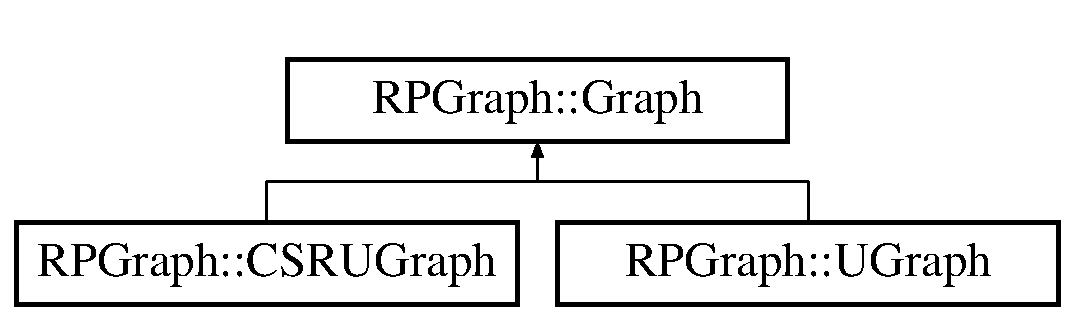
\includegraphics[height=2.000000cm]{classRPGraph_1_1Graph}
\end{center}
\end{figure}
\subsection*{Public Member Functions}
\begin{DoxyCompactItemize}
\item 
virtual \mbox{\hyperlink{namespaceRPGraph_ab3ae34f1ab88e48f43794c30c8697b74}{nid\+\_\+t}} \mbox{\hyperlink{classRPGraph_1_1Graph_ab5602e6b776a0ea3b944775331fcb2aa}{num\+\_\+nodes}} ()=0
\item 
virtual \mbox{\hyperlink{namespaceRPGraph_ab3ae34f1ab88e48f43794c30c8697b74}{nid\+\_\+t}} \mbox{\hyperlink{classRPGraph_1_1Graph_acd3b877216686aff2f7fbc2d62bcdf9b}{num\+\_\+edges}} ()=0
\item 
virtual \mbox{\hyperlink{namespaceRPGraph_ab3ae34f1ab88e48f43794c30c8697b74}{nid\+\_\+t}} \mbox{\hyperlink{classRPGraph_1_1Graph_a8a95d1f403c3d9860cf7399abc820c7d}{degree}} (\mbox{\hyperlink{namespaceRPGraph_ab3ae34f1ab88e48f43794c30c8697b74}{nid\+\_\+t}} nid)=0
\item 
virtual \mbox{\hyperlink{namespaceRPGraph_ab3ae34f1ab88e48f43794c30c8697b74}{nid\+\_\+t}} \mbox{\hyperlink{classRPGraph_1_1Graph_ab75e19f698a4ab99e37593c7178f2c1a}{in\+\_\+degree}} (\mbox{\hyperlink{namespaceRPGraph_ab3ae34f1ab88e48f43794c30c8697b74}{nid\+\_\+t}} nid)=0
\item 
virtual \mbox{\hyperlink{namespaceRPGraph_ab3ae34f1ab88e48f43794c30c8697b74}{nid\+\_\+t}} \mbox{\hyperlink{classRPGraph_1_1Graph_a660ad58e03df7e3cc00d0eb4e5c16819}{out\+\_\+degree}} (\mbox{\hyperlink{namespaceRPGraph_ab3ae34f1ab88e48f43794c30c8697b74}{nid\+\_\+t}} nid)=0
\item 
virtual std\+::vector$<$ \mbox{\hyperlink{namespaceRPGraph_ab3ae34f1ab88e48f43794c30c8697b74}{nid\+\_\+t}} $>$ \mbox{\hyperlink{classRPGraph_1_1Graph_ab1e27e4268d36443a5db035fa7635cad}{neighbors\+\_\+with\+\_\+geq\+\_\+id}} (\mbox{\hyperlink{namespaceRPGraph_ab3ae34f1ab88e48f43794c30c8697b74}{nid\+\_\+t}} nid)=0
\end{DoxyCompactItemize}


\subsection{Member Function Documentation}
\mbox{\Hypertarget{classRPGraph_1_1Graph_a8a95d1f403c3d9860cf7399abc820c7d}\label{classRPGraph_1_1Graph_a8a95d1f403c3d9860cf7399abc820c7d}} 
\index{R\+P\+Graph\+::\+Graph@{R\+P\+Graph\+::\+Graph}!degree@{degree}}
\index{degree@{degree}!R\+P\+Graph\+::\+Graph@{R\+P\+Graph\+::\+Graph}}
\subsubsection{\texorpdfstring{degree()}{degree()}}
{\footnotesize\ttfamily virtual \mbox{\hyperlink{namespaceRPGraph_ab3ae34f1ab88e48f43794c30c8697b74}{nid\+\_\+t}} R\+P\+Graph\+::\+Graph\+::degree (\begin{DoxyParamCaption}\item[{\mbox{\hyperlink{namespaceRPGraph_ab3ae34f1ab88e48f43794c30c8697b74}{nid\+\_\+t}}}]{nid }\end{DoxyParamCaption})\hspace{0.3cm}{\ttfamily [pure virtual]}}



Implemented in \mbox{\hyperlink{classRPGraph_1_1CSRUGraph_ae2f3bb7a5ee2b53c88145a0cee6ed277}{R\+P\+Graph\+::\+C\+S\+R\+U\+Graph}}, and \mbox{\hyperlink{classRPGraph_1_1UGraph_a4d3c3af1ba4787ef5ced5f5efa9d05cf}{R\+P\+Graph\+::\+U\+Graph}}.

\mbox{\Hypertarget{classRPGraph_1_1Graph_ab75e19f698a4ab99e37593c7178f2c1a}\label{classRPGraph_1_1Graph_ab75e19f698a4ab99e37593c7178f2c1a}} 
\index{R\+P\+Graph\+::\+Graph@{R\+P\+Graph\+::\+Graph}!in\+\_\+degree@{in\+\_\+degree}}
\index{in\+\_\+degree@{in\+\_\+degree}!R\+P\+Graph\+::\+Graph@{R\+P\+Graph\+::\+Graph}}
\subsubsection{\texorpdfstring{in\+\_\+degree()}{in\_degree()}}
{\footnotesize\ttfamily virtual \mbox{\hyperlink{namespaceRPGraph_ab3ae34f1ab88e48f43794c30c8697b74}{nid\+\_\+t}} R\+P\+Graph\+::\+Graph\+::in\+\_\+degree (\begin{DoxyParamCaption}\item[{\mbox{\hyperlink{namespaceRPGraph_ab3ae34f1ab88e48f43794c30c8697b74}{nid\+\_\+t}}}]{nid }\end{DoxyParamCaption})\hspace{0.3cm}{\ttfamily [pure virtual]}}



Implemented in \mbox{\hyperlink{classRPGraph_1_1CSRUGraph_a88965d72f2fbea43b6d731d2cc027858}{R\+P\+Graph\+::\+C\+S\+R\+U\+Graph}}, and \mbox{\hyperlink{classRPGraph_1_1UGraph_a5614092aab1bb8d92b625506f944d39c}{R\+P\+Graph\+::\+U\+Graph}}.

\mbox{\Hypertarget{classRPGraph_1_1Graph_ab1e27e4268d36443a5db035fa7635cad}\label{classRPGraph_1_1Graph_ab1e27e4268d36443a5db035fa7635cad}} 
\index{R\+P\+Graph\+::\+Graph@{R\+P\+Graph\+::\+Graph}!neighbors\+\_\+with\+\_\+geq\+\_\+id@{neighbors\+\_\+with\+\_\+geq\+\_\+id}}
\index{neighbors\+\_\+with\+\_\+geq\+\_\+id@{neighbors\+\_\+with\+\_\+geq\+\_\+id}!R\+P\+Graph\+::\+Graph@{R\+P\+Graph\+::\+Graph}}
\subsubsection{\texorpdfstring{neighbors\+\_\+with\+\_\+geq\+\_\+id()}{neighbors\_with\_geq\_id()}}
{\footnotesize\ttfamily virtual std\+::vector$<$\mbox{\hyperlink{namespaceRPGraph_ab3ae34f1ab88e48f43794c30c8697b74}{nid\+\_\+t}}$>$ R\+P\+Graph\+::\+Graph\+::neighbors\+\_\+with\+\_\+geq\+\_\+id (\begin{DoxyParamCaption}\item[{\mbox{\hyperlink{namespaceRPGraph_ab3ae34f1ab88e48f43794c30c8697b74}{nid\+\_\+t}}}]{nid }\end{DoxyParamCaption})\hspace{0.3cm}{\ttfamily [pure virtual]}}



Implemented in \mbox{\hyperlink{classRPGraph_1_1UGraph_a8cc5be5cfd41f351d4f98de816028f90}{R\+P\+Graph\+::\+U\+Graph}}.

\mbox{\Hypertarget{classRPGraph_1_1Graph_acd3b877216686aff2f7fbc2d62bcdf9b}\label{classRPGraph_1_1Graph_acd3b877216686aff2f7fbc2d62bcdf9b}} 
\index{R\+P\+Graph\+::\+Graph@{R\+P\+Graph\+::\+Graph}!num\+\_\+edges@{num\+\_\+edges}}
\index{num\+\_\+edges@{num\+\_\+edges}!R\+P\+Graph\+::\+Graph@{R\+P\+Graph\+::\+Graph}}
\subsubsection{\texorpdfstring{num\+\_\+edges()}{num\_edges()}}
{\footnotesize\ttfamily virtual \mbox{\hyperlink{namespaceRPGraph_ab3ae34f1ab88e48f43794c30c8697b74}{nid\+\_\+t}} R\+P\+Graph\+::\+Graph\+::num\+\_\+edges (\begin{DoxyParamCaption}{ }\end{DoxyParamCaption})\hspace{0.3cm}{\ttfamily [pure virtual]}}



Implemented in \mbox{\hyperlink{classRPGraph_1_1CSRUGraph_a90ef3e196b0e234c8806bc455031018d}{R\+P\+Graph\+::\+C\+S\+R\+U\+Graph}}, and \mbox{\hyperlink{classRPGraph_1_1UGraph_a55a5deea9a4d456e78e24a2002f31ef2}{R\+P\+Graph\+::\+U\+Graph}}.

\mbox{\Hypertarget{classRPGraph_1_1Graph_ab5602e6b776a0ea3b944775331fcb2aa}\label{classRPGraph_1_1Graph_ab5602e6b776a0ea3b944775331fcb2aa}} 
\index{R\+P\+Graph\+::\+Graph@{R\+P\+Graph\+::\+Graph}!num\+\_\+nodes@{num\+\_\+nodes}}
\index{num\+\_\+nodes@{num\+\_\+nodes}!R\+P\+Graph\+::\+Graph@{R\+P\+Graph\+::\+Graph}}
\subsubsection{\texorpdfstring{num\+\_\+nodes()}{num\_nodes()}}
{\footnotesize\ttfamily virtual \mbox{\hyperlink{namespaceRPGraph_ab3ae34f1ab88e48f43794c30c8697b74}{nid\+\_\+t}} R\+P\+Graph\+::\+Graph\+::num\+\_\+nodes (\begin{DoxyParamCaption}{ }\end{DoxyParamCaption})\hspace{0.3cm}{\ttfamily [pure virtual]}}



Implemented in \mbox{\hyperlink{classRPGraph_1_1CSRUGraph_a715af46d35bbe09b6b7d724461a1c2a5}{R\+P\+Graph\+::\+C\+S\+R\+U\+Graph}}, and \mbox{\hyperlink{classRPGraph_1_1UGraph_ad5eb18fffb7b9a64819b3f1f38305a0c}{R\+P\+Graph\+::\+U\+Graph}}.

\mbox{\Hypertarget{classRPGraph_1_1Graph_a660ad58e03df7e3cc00d0eb4e5c16819}\label{classRPGraph_1_1Graph_a660ad58e03df7e3cc00d0eb4e5c16819}} 
\index{R\+P\+Graph\+::\+Graph@{R\+P\+Graph\+::\+Graph}!out\+\_\+degree@{out\+\_\+degree}}
\index{out\+\_\+degree@{out\+\_\+degree}!R\+P\+Graph\+::\+Graph@{R\+P\+Graph\+::\+Graph}}
\subsubsection{\texorpdfstring{out\+\_\+degree()}{out\_degree()}}
{\footnotesize\ttfamily virtual \mbox{\hyperlink{namespaceRPGraph_ab3ae34f1ab88e48f43794c30c8697b74}{nid\+\_\+t}} R\+P\+Graph\+::\+Graph\+::out\+\_\+degree (\begin{DoxyParamCaption}\item[{\mbox{\hyperlink{namespaceRPGraph_ab3ae34f1ab88e48f43794c30c8697b74}{nid\+\_\+t}}}]{nid }\end{DoxyParamCaption})\hspace{0.3cm}{\ttfamily [pure virtual]}}



Implemented in \mbox{\hyperlink{classRPGraph_1_1CSRUGraph_a952e2a8eea28c0d879a0b5688d0e1b06}{R\+P\+Graph\+::\+C\+S\+R\+U\+Graph}}, and \mbox{\hyperlink{classRPGraph_1_1UGraph_a8416a5fa8b87b8569d0fa563288ac162}{R\+P\+Graph\+::\+U\+Graph}}.



The documentation for this class was generated from the following file\+:\begin{DoxyCompactItemize}
\item 
\mbox{\hyperlink{RPGraph_8hpp}{R\+P\+Graph.\+hpp}}\end{DoxyCompactItemize}

\hypertarget{classRPGraph_1_1GraphLayout}{}\section{R\+P\+Graph\+:\+:Graph\+Layout Class Reference}
\label{classRPGraph_1_1GraphLayout}\index{R\+P\+Graph\+::\+Graph\+Layout@{R\+P\+Graph\+::\+Graph\+Layout}}


{\ttfamily \#include $<$R\+P\+Graph\+Layout.\+hpp$>$}

\subsection*{Public Member Functions}
\begin{DoxyCompactItemize}
\item 
\mbox{\hyperlink{classRPGraph_1_1GraphLayout_a3d1840f5ef30c9c7a6ce5d41b54230ef}{Graph\+Layout}} (\mbox{\hyperlink{classRPGraph_1_1UGraph}{R\+P\+Graph\+::\+U\+Graph}} \&\mbox{\hyperlink{classRPGraph_1_1GraphLayout_af44bb2c10eee4ef67c95355ce93432a5}{graph}}, float \mbox{\hyperlink{classRPGraph_1_1GraphLayout_ade29dd5ff17faff96348650a99bd120c}{width}}=10000, float \mbox{\hyperlink{classRPGraph_1_1GraphLayout_a86a79a0329c88ef7cef8d57fce9f0e1b}{height}}=10000)
\item 
\mbox{\hyperlink{classRPGraph_1_1GraphLayout_a284707481e0ba81f1dec33a03bc1293c}{$\sim$\+Graph\+Layout}} ()
\item 
void \mbox{\hyperlink{classRPGraph_1_1GraphLayout_a5d5912f46f1b6bf1bf1ee5850cbd818e}{randomize\+Positions}} ()
\item 
float \mbox{\hyperlink{classRPGraph_1_1GraphLayout_a447d80a00c47ad2fb446e3653face38c}{getX}} (\mbox{\hyperlink{namespaceRPGraph_ab3ae34f1ab88e48f43794c30c8697b74}{nid\+\_\+t}} node\+\_\+id)
\item 
float \mbox{\hyperlink{classRPGraph_1_1GraphLayout_a75826cfc0cc24fd4902758bc1ad42c4b}{getY}} (\mbox{\hyperlink{namespaceRPGraph_ab3ae34f1ab88e48f43794c30c8697b74}{nid\+\_\+t}} node\+\_\+id)
\item 
float \mbox{\hyperlink{classRPGraph_1_1GraphLayout_a18a15867788b88db16f0938540107748}{get\+X\+Range}} ()
\item 
float \mbox{\hyperlink{classRPGraph_1_1GraphLayout_aeba4c2af91bcc996e159eebbb049c276}{get\+Y\+Range}} ()
\item 
float \mbox{\hyperlink{classRPGraph_1_1GraphLayout_a805e477534bbf72275ecf8d5ec396da4}{get\+Span}} ()
\item 
float \mbox{\hyperlink{classRPGraph_1_1GraphLayout_abdfcbd0f0fea5c5fdf237a7dc653ca13}{get\+Distance}} (\mbox{\hyperlink{namespaceRPGraph_ab3ae34f1ab88e48f43794c30c8697b74}{nid\+\_\+t}} n1, \mbox{\hyperlink{namespaceRPGraph_ab3ae34f1ab88e48f43794c30c8697b74}{nid\+\_\+t}} n2)
\item 
\mbox{\hyperlink{classRPGraph_1_1Real2DVector}{Real2\+D\+Vector}} \mbox{\hyperlink{classRPGraph_1_1GraphLayout_af90cdf14a0bfea5e6854ba1b2b885761}{get\+Distance\+Vector}} (\mbox{\hyperlink{namespaceRPGraph_ab3ae34f1ab88e48f43794c30c8697b74}{nid\+\_\+t}} n1, \mbox{\hyperlink{namespaceRPGraph_ab3ae34f1ab88e48f43794c30c8697b74}{nid\+\_\+t}} n2)
\item 
\mbox{\hyperlink{classRPGraph_1_1Real2DVector}{Real2\+D\+Vector}} \mbox{\hyperlink{classRPGraph_1_1GraphLayout_a3e3e2ba138f5b416a32f52d957926da5}{get\+Normalized\+Distance\+Vector}} (\mbox{\hyperlink{namespaceRPGraph_ab3ae34f1ab88e48f43794c30c8697b74}{nid\+\_\+t}} n1, \mbox{\hyperlink{namespaceRPGraph_ab3ae34f1ab88e48f43794c30c8697b74}{nid\+\_\+t}} n2)
\item 
\mbox{\hyperlink{classRPGraph_1_1Coordinate}{Coordinate}} \mbox{\hyperlink{classRPGraph_1_1GraphLayout_a069b03de122b6dd8e7518db18d7615c9}{get\+Coordinate}} (\mbox{\hyperlink{namespaceRPGraph_ab3ae34f1ab88e48f43794c30c8697b74}{nid\+\_\+t}} node\+\_\+id)
\item 
\mbox{\hyperlink{classRPGraph_1_1Coordinate}{Coordinate}} \mbox{\hyperlink{classRPGraph_1_1GraphLayout_aa9a3cfeb1f895fce3c9b352200251d5f}{get\+Center}} ()
\item 
void \mbox{\hyperlink{classRPGraph_1_1GraphLayout_a870e6ad8d7e2dab189cb591dead19414}{setX}} (\mbox{\hyperlink{namespaceRPGraph_ab3ae34f1ab88e48f43794c30c8697b74}{nid\+\_\+t}} node\+\_\+id, float x\+\_\+value)
\item 
void \mbox{\hyperlink{classRPGraph_1_1GraphLayout_a55203ccaaba03d4dd739c2e6552be90e}{setY}} (\mbox{\hyperlink{namespaceRPGraph_ab3ae34f1ab88e48f43794c30c8697b74}{nid\+\_\+t}} node\+\_\+id, float y\+\_\+value)
\item 
void \mbox{\hyperlink{classRPGraph_1_1GraphLayout_a00198f453c2216d63e3afcbf8eed0122}{move\+Node}} (\mbox{\hyperlink{namespaceRPGraph_ab3ae34f1ab88e48f43794c30c8697b74}{nid\+\_\+t}}, \mbox{\hyperlink{classRPGraph_1_1Real2DVector}{Real2\+D\+Vector}} v)
\item 
void \mbox{\hyperlink{classRPGraph_1_1GraphLayout_a99ad68f3edff2c5f0a78a4db3e2f15ea}{set\+Coordinates}} (\mbox{\hyperlink{namespaceRPGraph_ab3ae34f1ab88e48f43794c30c8697b74}{nid\+\_\+t}} node\+\_\+id, \mbox{\hyperlink{classRPGraph_1_1Coordinate}{Coordinate}} c)
\item 
void \mbox{\hyperlink{classRPGraph_1_1GraphLayout_ab5892ee9d2eba41d1f285f0e480d00e2}{write\+To\+P\+NG}} (const int image\+\_\+w, const int image\+\_\+h, std\+::string path)
\item 
void \mbox{\hyperlink{classRPGraph_1_1GraphLayout_ae01b3ad2b348683c2e55d49496c32800}{write\+To\+C\+SV}} (std\+::string path)
\item 
void \mbox{\hyperlink{classRPGraph_1_1GraphLayout_a19fb67898bdb294ac46fb098ec2b0bad}{write\+To\+Bin}} (std\+::string path)
\end{DoxyCompactItemize}
\subsection*{Public Attributes}
\begin{DoxyCompactItemize}
\item 
\mbox{\hyperlink{classRPGraph_1_1UGraph}{U\+Graph}} \& \mbox{\hyperlink{classRPGraph_1_1GraphLayout_af44bb2c10eee4ef67c95355ce93432a5}{graph}}
\end{DoxyCompactItemize}
\subsection*{Protected Member Functions}
\begin{DoxyCompactItemize}
\item 
float \mbox{\hyperlink{classRPGraph_1_1GraphLayout_a9b538f82aabafa2d2f0e1a08edcf9b85}{minX}} ()
\item 
float \mbox{\hyperlink{classRPGraph_1_1GraphLayout_adc5cd076f816ecca32c91c4fe3a2a57e}{minY}} ()
\item 
float \mbox{\hyperlink{classRPGraph_1_1GraphLayout_a6ec496912efecaa34efd4de6d88fc505}{maxX}} ()
\item 
float \mbox{\hyperlink{classRPGraph_1_1GraphLayout_a031dd59e25111ed175d6153d2cb44f9a}{maxY}} ()
\end{DoxyCompactItemize}
\subsection*{Protected Attributes}
\begin{DoxyCompactItemize}
\item 
float \mbox{\hyperlink{classRPGraph_1_1GraphLayout_ade29dd5ff17faff96348650a99bd120c}{width}}
\item 
float \mbox{\hyperlink{classRPGraph_1_1GraphLayout_a86a79a0329c88ef7cef8d57fce9f0e1b}{height}}
\end{DoxyCompactItemize}


\subsection{Constructor \& Destructor Documentation}
\mbox{\Hypertarget{classRPGraph_1_1GraphLayout_a3d1840f5ef30c9c7a6ce5d41b54230ef}\label{classRPGraph_1_1GraphLayout_a3d1840f5ef30c9c7a6ce5d41b54230ef}} 
\index{R\+P\+Graph\+::\+Graph\+Layout@{R\+P\+Graph\+::\+Graph\+Layout}!Graph\+Layout@{Graph\+Layout}}
\index{Graph\+Layout@{Graph\+Layout}!R\+P\+Graph\+::\+Graph\+Layout@{R\+P\+Graph\+::\+Graph\+Layout}}
\subsubsection{\texorpdfstring{Graph\+Layout()}{GraphLayout()}}
{\footnotesize\ttfamily R\+P\+Graph\+::\+Graph\+Layout\+::\+Graph\+Layout (\begin{DoxyParamCaption}\item[{\mbox{\hyperlink{classRPGraph_1_1UGraph}{R\+P\+Graph\+::\+U\+Graph}} \&}]{graph,  }\item[{float}]{width = {\ttfamily 10000},  }\item[{float}]{height = {\ttfamily 10000} }\end{DoxyParamCaption})}

Q\+: What are width and height for? Size of image? \mbox{\Hypertarget{classRPGraph_1_1GraphLayout_a284707481e0ba81f1dec33a03bc1293c}\label{classRPGraph_1_1GraphLayout_a284707481e0ba81f1dec33a03bc1293c}} 
\index{R\+P\+Graph\+::\+Graph\+Layout@{R\+P\+Graph\+::\+Graph\+Layout}!````~Graph\+Layout@{$\sim$\+Graph\+Layout}}
\index{````~Graph\+Layout@{$\sim$\+Graph\+Layout}!R\+P\+Graph\+::\+Graph\+Layout@{R\+P\+Graph\+::\+Graph\+Layout}}
\subsubsection{\texorpdfstring{$\sim$\+Graph\+Layout()}{~GraphLayout()}}
{\footnotesize\ttfamily R\+P\+Graph\+::\+Graph\+Layout\+::$\sim$\+Graph\+Layout (\begin{DoxyParamCaption}{ }\end{DoxyParamCaption})}



\subsection{Member Function Documentation}
\mbox{\Hypertarget{classRPGraph_1_1GraphLayout_aa9a3cfeb1f895fce3c9b352200251d5f}\label{classRPGraph_1_1GraphLayout_aa9a3cfeb1f895fce3c9b352200251d5f}} 
\index{R\+P\+Graph\+::\+Graph\+Layout@{R\+P\+Graph\+::\+Graph\+Layout}!get\+Center@{get\+Center}}
\index{get\+Center@{get\+Center}!R\+P\+Graph\+::\+Graph\+Layout@{R\+P\+Graph\+::\+Graph\+Layout}}
\subsubsection{\texorpdfstring{get\+Center()}{getCenter()}}
{\footnotesize\ttfamily \mbox{\hyperlink{classRPGraph_1_1Coordinate}{Coordinate}} R\+P\+Graph\+::\+Graph\+Layout\+::get\+Center (\begin{DoxyParamCaption}{ }\end{DoxyParamCaption})}

Usage\+: pngwriter only. \mbox{\Hypertarget{classRPGraph_1_1GraphLayout_a069b03de122b6dd8e7518db18d7615c9}\label{classRPGraph_1_1GraphLayout_a069b03de122b6dd8e7518db18d7615c9}} 
\index{R\+P\+Graph\+::\+Graph\+Layout@{R\+P\+Graph\+::\+Graph\+Layout}!get\+Coordinate@{get\+Coordinate}}
\index{get\+Coordinate@{get\+Coordinate}!R\+P\+Graph\+::\+Graph\+Layout@{R\+P\+Graph\+::\+Graph\+Layout}}
\subsubsection{\texorpdfstring{get\+Coordinate()}{getCoordinate()}}
{\footnotesize\ttfamily \mbox{\hyperlink{classRPGraph_1_1Coordinate}{Coordinate}} R\+P\+Graph\+::\+Graph\+Layout\+::get\+Coordinate (\begin{DoxyParamCaption}\item[{\mbox{\hyperlink{namespaceRPGraph_ab3ae34f1ab88e48f43794c30c8697b74}{nid\+\_\+t}}}]{node\+\_\+id }\end{DoxyParamCaption})}

Indexes into coordinates array. \mbox{\Hypertarget{classRPGraph_1_1GraphLayout_abdfcbd0f0fea5c5fdf237a7dc653ca13}\label{classRPGraph_1_1GraphLayout_abdfcbd0f0fea5c5fdf237a7dc653ca13}} 
\index{R\+P\+Graph\+::\+Graph\+Layout@{R\+P\+Graph\+::\+Graph\+Layout}!get\+Distance@{get\+Distance}}
\index{get\+Distance@{get\+Distance}!R\+P\+Graph\+::\+Graph\+Layout@{R\+P\+Graph\+::\+Graph\+Layout}}
\subsubsection{\texorpdfstring{get\+Distance()}{getDistance()}}
{\footnotesize\ttfamily float R\+P\+Graph\+::\+Graph\+Layout\+::get\+Distance (\begin{DoxyParamCaption}\item[{\mbox{\hyperlink{namespaceRPGraph_ab3ae34f1ab88e48f43794c30c8697b74}{nid\+\_\+t}}}]{n1,  }\item[{\mbox{\hyperlink{namespaceRPGraph_ab3ae34f1ab88e48f43794c30c8697b74}{nid\+\_\+t}}}]{n2 }\end{DoxyParamCaption})}

Usage? C\+PU F\+A2 only. \mbox{\Hypertarget{classRPGraph_1_1GraphLayout_af90cdf14a0bfea5e6854ba1b2b885761}\label{classRPGraph_1_1GraphLayout_af90cdf14a0bfea5e6854ba1b2b885761}} 
\index{R\+P\+Graph\+::\+Graph\+Layout@{R\+P\+Graph\+::\+Graph\+Layout}!get\+Distance\+Vector@{get\+Distance\+Vector}}
\index{get\+Distance\+Vector@{get\+Distance\+Vector}!R\+P\+Graph\+::\+Graph\+Layout@{R\+P\+Graph\+::\+Graph\+Layout}}
\subsubsection{\texorpdfstring{get\+Distance\+Vector()}{getDistanceVector()}}
{\footnotesize\ttfamily \mbox{\hyperlink{classRPGraph_1_1Real2DVector}{Real2\+D\+Vector}} R\+P\+Graph\+::\+Graph\+Layout\+::get\+Distance\+Vector (\begin{DoxyParamCaption}\item[{\mbox{\hyperlink{namespaceRPGraph_ab3ae34f1ab88e48f43794c30c8697b74}{nid\+\_\+t}}}]{n1,  }\item[{\mbox{\hyperlink{namespaceRPGraph_ab3ae34f1ab88e48f43794c30c8697b74}{nid\+\_\+t}}}]{n2 }\end{DoxyParamCaption})}

Which of these 2 are used? Vectors are used in C\+PU F\+A2 implementation. \mbox{\Hypertarget{classRPGraph_1_1GraphLayout_a3e3e2ba138f5b416a32f52d957926da5}\label{classRPGraph_1_1GraphLayout_a3e3e2ba138f5b416a32f52d957926da5}} 
\index{R\+P\+Graph\+::\+Graph\+Layout@{R\+P\+Graph\+::\+Graph\+Layout}!get\+Normalized\+Distance\+Vector@{get\+Normalized\+Distance\+Vector}}
\index{get\+Normalized\+Distance\+Vector@{get\+Normalized\+Distance\+Vector}!R\+P\+Graph\+::\+Graph\+Layout@{R\+P\+Graph\+::\+Graph\+Layout}}
\subsubsection{\texorpdfstring{get\+Normalized\+Distance\+Vector()}{getNormalizedDistanceVector()}}
{\footnotesize\ttfamily \mbox{\hyperlink{classRPGraph_1_1Real2DVector}{Real2\+D\+Vector}} R\+P\+Graph\+::\+Graph\+Layout\+::get\+Normalized\+Distance\+Vector (\begin{DoxyParamCaption}\item[{\mbox{\hyperlink{namespaceRPGraph_ab3ae34f1ab88e48f43794c30c8697b74}{nid\+\_\+t}}}]{n1,  }\item[{\mbox{\hyperlink{namespaceRPGraph_ab3ae34f1ab88e48f43794c30c8697b74}{nid\+\_\+t}}}]{n2 }\end{DoxyParamCaption})}

Make that which of these 3 are used? I\+R\+R\+E\+L\+E\+V\+A\+NT\+: Commented out in C\+PU F\+A2 only. \mbox{\Hypertarget{classRPGraph_1_1GraphLayout_a805e477534bbf72275ecf8d5ec396da4}\label{classRPGraph_1_1GraphLayout_a805e477534bbf72275ecf8d5ec396da4}} 
\index{R\+P\+Graph\+::\+Graph\+Layout@{R\+P\+Graph\+::\+Graph\+Layout}!get\+Span@{get\+Span}}
\index{get\+Span@{get\+Span}!R\+P\+Graph\+::\+Graph\+Layout@{R\+P\+Graph\+::\+Graph\+Layout}}
\subsubsection{\texorpdfstring{get\+Span()}{getSpan()}}
{\footnotesize\ttfamily float R\+P\+Graph\+::\+Graph\+Layout\+::get\+Span (\begin{DoxyParamCaption}{ }\end{DoxyParamCaption})}

\mbox{\Hypertarget{classRPGraph_1_1GraphLayout_a447d80a00c47ad2fb446e3653face38c}\label{classRPGraph_1_1GraphLayout_a447d80a00c47ad2fb446e3653face38c}} 
\index{R\+P\+Graph\+::\+Graph\+Layout@{R\+P\+Graph\+::\+Graph\+Layout}!getX@{getX}}
\index{getX@{getX}!R\+P\+Graph\+::\+Graph\+Layout@{R\+P\+Graph\+::\+Graph\+Layout}}
\subsubsection{\texorpdfstring{get\+X()}{getX()}}
{\footnotesize\ttfamily float R\+P\+Graph\+::\+Graph\+Layout\+::getX (\begin{DoxyParamCaption}\item[{\mbox{\hyperlink{namespaceRPGraph_ab3ae34f1ab88e48f43794c30c8697b74}{nid\+\_\+t}}}]{node\+\_\+id }\end{DoxyParamCaption})}

\mbox{\Hypertarget{classRPGraph_1_1GraphLayout_a18a15867788b88db16f0938540107748}\label{classRPGraph_1_1GraphLayout_a18a15867788b88db16f0938540107748}} 
\index{R\+P\+Graph\+::\+Graph\+Layout@{R\+P\+Graph\+::\+Graph\+Layout}!get\+X\+Range@{get\+X\+Range}}
\index{get\+X\+Range@{get\+X\+Range}!R\+P\+Graph\+::\+Graph\+Layout@{R\+P\+Graph\+::\+Graph\+Layout}}
\subsubsection{\texorpdfstring{get\+X\+Range()}{getXRange()}}
{\footnotesize\ttfamily float R\+P\+Graph\+::\+Graph\+Layout\+::get\+X\+Range (\begin{DoxyParamCaption}{ }\end{DoxyParamCaption})}

\mbox{\Hypertarget{classRPGraph_1_1GraphLayout_a75826cfc0cc24fd4902758bc1ad42c4b}\label{classRPGraph_1_1GraphLayout_a75826cfc0cc24fd4902758bc1ad42c4b}} 
\index{R\+P\+Graph\+::\+Graph\+Layout@{R\+P\+Graph\+::\+Graph\+Layout}!getY@{getY}}
\index{getY@{getY}!R\+P\+Graph\+::\+Graph\+Layout@{R\+P\+Graph\+::\+Graph\+Layout}}
\subsubsection{\texorpdfstring{get\+Y()}{getY()}}
{\footnotesize\ttfamily float R\+P\+Graph\+::\+Graph\+Layout\+::getY (\begin{DoxyParamCaption}\item[{\mbox{\hyperlink{namespaceRPGraph_ab3ae34f1ab88e48f43794c30c8697b74}{nid\+\_\+t}}}]{node\+\_\+id }\end{DoxyParamCaption})}

\mbox{\Hypertarget{classRPGraph_1_1GraphLayout_aeba4c2af91bcc996e159eebbb049c276}\label{classRPGraph_1_1GraphLayout_aeba4c2af91bcc996e159eebbb049c276}} 
\index{R\+P\+Graph\+::\+Graph\+Layout@{R\+P\+Graph\+::\+Graph\+Layout}!get\+Y\+Range@{get\+Y\+Range}}
\index{get\+Y\+Range@{get\+Y\+Range}!R\+P\+Graph\+::\+Graph\+Layout@{R\+P\+Graph\+::\+Graph\+Layout}}
\subsubsection{\texorpdfstring{get\+Y\+Range()}{getYRange()}}
{\footnotesize\ttfamily float R\+P\+Graph\+::\+Graph\+Layout\+::get\+Y\+Range (\begin{DoxyParamCaption}{ }\end{DoxyParamCaption})}

\mbox{\Hypertarget{classRPGraph_1_1GraphLayout_a6ec496912efecaa34efd4de6d88fc505}\label{classRPGraph_1_1GraphLayout_a6ec496912efecaa34efd4de6d88fc505}} 
\index{R\+P\+Graph\+::\+Graph\+Layout@{R\+P\+Graph\+::\+Graph\+Layout}!maxX@{maxX}}
\index{maxX@{maxX}!R\+P\+Graph\+::\+Graph\+Layout@{R\+P\+Graph\+::\+Graph\+Layout}}
\subsubsection{\texorpdfstring{max\+X()}{maxX()}}
{\footnotesize\ttfamily float R\+P\+Graph\+::\+Graph\+Layout\+::maxX (\begin{DoxyParamCaption}{ }\end{DoxyParamCaption})\hspace{0.3cm}{\ttfamily [protected]}}

\mbox{\Hypertarget{classRPGraph_1_1GraphLayout_a031dd59e25111ed175d6153d2cb44f9a}\label{classRPGraph_1_1GraphLayout_a031dd59e25111ed175d6153d2cb44f9a}} 
\index{R\+P\+Graph\+::\+Graph\+Layout@{R\+P\+Graph\+::\+Graph\+Layout}!maxY@{maxY}}
\index{maxY@{maxY}!R\+P\+Graph\+::\+Graph\+Layout@{R\+P\+Graph\+::\+Graph\+Layout}}
\subsubsection{\texorpdfstring{max\+Y()}{maxY()}}
{\footnotesize\ttfamily float R\+P\+Graph\+::\+Graph\+Layout\+::maxY (\begin{DoxyParamCaption}{ }\end{DoxyParamCaption})\hspace{0.3cm}{\ttfamily [protected]}}

\mbox{\Hypertarget{classRPGraph_1_1GraphLayout_a9b538f82aabafa2d2f0e1a08edcf9b85}\label{classRPGraph_1_1GraphLayout_a9b538f82aabafa2d2f0e1a08edcf9b85}} 
\index{R\+P\+Graph\+::\+Graph\+Layout@{R\+P\+Graph\+::\+Graph\+Layout}!minX@{minX}}
\index{minX@{minX}!R\+P\+Graph\+::\+Graph\+Layout@{R\+P\+Graph\+::\+Graph\+Layout}}
\subsubsection{\texorpdfstring{min\+X()}{minX()}}
{\footnotesize\ttfamily float R\+P\+Graph\+::\+Graph\+Layout\+::minX (\begin{DoxyParamCaption}{ }\end{DoxyParamCaption})\hspace{0.3cm}{\ttfamily [protected]}}

Find\+: get\+X\+Range\+: only this file, get\+Span, get\+Center, write\+Png get\+Y\+Range\+: only this file get\+Center\+: \mbox{\hyperlink{RPCPUForceAtlas2_8cpp}{R\+P\+C\+P\+U\+Force\+Atlas2.\+cpp}}, not important \mbox{\Hypertarget{classRPGraph_1_1GraphLayout_adc5cd076f816ecca32c91c4fe3a2a57e}\label{classRPGraph_1_1GraphLayout_adc5cd076f816ecca32c91c4fe3a2a57e}} 
\index{R\+P\+Graph\+::\+Graph\+Layout@{R\+P\+Graph\+::\+Graph\+Layout}!minY@{minY}}
\index{minY@{minY}!R\+P\+Graph\+::\+Graph\+Layout@{R\+P\+Graph\+::\+Graph\+Layout}}
\subsubsection{\texorpdfstring{min\+Y()}{minY()}}
{\footnotesize\ttfamily float R\+P\+Graph\+::\+Graph\+Layout\+::minY (\begin{DoxyParamCaption}{ }\end{DoxyParamCaption})\hspace{0.3cm}{\ttfamily [protected]}}

\mbox{\Hypertarget{classRPGraph_1_1GraphLayout_a00198f453c2216d63e3afcbf8eed0122}\label{classRPGraph_1_1GraphLayout_a00198f453c2216d63e3afcbf8eed0122}} 
\index{R\+P\+Graph\+::\+Graph\+Layout@{R\+P\+Graph\+::\+Graph\+Layout}!move\+Node@{move\+Node}}
\index{move\+Node@{move\+Node}!R\+P\+Graph\+::\+Graph\+Layout@{R\+P\+Graph\+::\+Graph\+Layout}}
\subsubsection{\texorpdfstring{move\+Node()}{moveNode()}}
{\footnotesize\ttfamily void R\+P\+Graph\+::\+Graph\+Layout\+::move\+Node (\begin{DoxyParamCaption}\item[{\mbox{\hyperlink{namespaceRPGraph_ab3ae34f1ab88e48f43794c30c8697b74}{nid\+\_\+t}}}]{n,  }\item[{\mbox{\hyperlink{classRPGraph_1_1Real2DVector}{R\+P\+Graph\+::\+Real2\+D\+Vector}}}]{v }\end{DoxyParamCaption})}

Why is move only used with a 2\+D\+Vector? \mbox{\Hypertarget{classRPGraph_1_1GraphLayout_a5d5912f46f1b6bf1bf1ee5850cbd818e}\label{classRPGraph_1_1GraphLayout_a5d5912f46f1b6bf1bf1ee5850cbd818e}} 
\index{R\+P\+Graph\+::\+Graph\+Layout@{R\+P\+Graph\+::\+Graph\+Layout}!randomize\+Positions@{randomize\+Positions}}
\index{randomize\+Positions@{randomize\+Positions}!R\+P\+Graph\+::\+Graph\+Layout@{R\+P\+Graph\+::\+Graph\+Layout}}
\subsubsection{\texorpdfstring{randomize\+Positions()}{randomizePositions()}}
{\footnotesize\ttfamily void R\+P\+Graph\+::\+Graph\+Layout\+::randomize\+Positions (\begin{DoxyParamCaption}{ }\end{DoxyParamCaption})}

T\+O\+DO\+: Modify this bit when using communities to randomize node positions within some delta of the community position in the community layout that was produced originally. N\+O\+TE\+: Keep original for laying out the community graph.\mbox{\Hypertarget{classRPGraph_1_1GraphLayout_a99ad68f3edff2c5f0a78a4db3e2f15ea}\label{classRPGraph_1_1GraphLayout_a99ad68f3edff2c5f0a78a4db3e2f15ea}} 
\index{R\+P\+Graph\+::\+Graph\+Layout@{R\+P\+Graph\+::\+Graph\+Layout}!set\+Coordinates@{set\+Coordinates}}
\index{set\+Coordinates@{set\+Coordinates}!R\+P\+Graph\+::\+Graph\+Layout@{R\+P\+Graph\+::\+Graph\+Layout}}
\subsubsection{\texorpdfstring{set\+Coordinates()}{setCoordinates()}}
{\footnotesize\ttfamily void R\+P\+Graph\+::\+Graph\+Layout\+::set\+Coordinates (\begin{DoxyParamCaption}\item[{\mbox{\hyperlink{namespaceRPGraph_ab3ae34f1ab88e48f43794c30c8697b74}{nid\+\_\+t}}}]{node\+\_\+id,  }\item[{\mbox{\hyperlink{classRPGraph_1_1Coordinate}{Coordinate}}}]{c }\end{DoxyParamCaption})}

Never used. Why not? T\+O\+DO\+: We will probably use this and maybe the move\+Node function to specify our layout after \mbox{\Hypertarget{classRPGraph_1_1GraphLayout_a870e6ad8d7e2dab189cb591dead19414}\label{classRPGraph_1_1GraphLayout_a870e6ad8d7e2dab189cb591dead19414}} 
\index{R\+P\+Graph\+::\+Graph\+Layout@{R\+P\+Graph\+::\+Graph\+Layout}!setX@{setX}}
\index{setX@{setX}!R\+P\+Graph\+::\+Graph\+Layout@{R\+P\+Graph\+::\+Graph\+Layout}}
\subsubsection{\texorpdfstring{set\+X()}{setX()}}
{\footnotesize\ttfamily void R\+P\+Graph\+::\+Graph\+Layout\+::setX (\begin{DoxyParamCaption}\item[{\mbox{\hyperlink{namespaceRPGraph_ab3ae34f1ab88e48f43794c30c8697b74}{nid\+\_\+t}}}]{node\+\_\+id,  }\item[{float}]{x\+\_\+value }\end{DoxyParamCaption})}

Updates x in coordinates array. \mbox{\Hypertarget{classRPGraph_1_1GraphLayout_a55203ccaaba03d4dd739c2e6552be90e}\label{classRPGraph_1_1GraphLayout_a55203ccaaba03d4dd739c2e6552be90e}} 
\index{R\+P\+Graph\+::\+Graph\+Layout@{R\+P\+Graph\+::\+Graph\+Layout}!setY@{setY}}
\index{setY@{setY}!R\+P\+Graph\+::\+Graph\+Layout@{R\+P\+Graph\+::\+Graph\+Layout}}
\subsubsection{\texorpdfstring{set\+Y()}{setY()}}
{\footnotesize\ttfamily void R\+P\+Graph\+::\+Graph\+Layout\+::setY (\begin{DoxyParamCaption}\item[{\mbox{\hyperlink{namespaceRPGraph_ab3ae34f1ab88e48f43794c30c8697b74}{nid\+\_\+t}}}]{node\+\_\+id,  }\item[{float}]{y\+\_\+value }\end{DoxyParamCaption})}

\mbox{\Hypertarget{classRPGraph_1_1GraphLayout_a19fb67898bdb294ac46fb098ec2b0bad}\label{classRPGraph_1_1GraphLayout_a19fb67898bdb294ac46fb098ec2b0bad}} 
\index{R\+P\+Graph\+::\+Graph\+Layout@{R\+P\+Graph\+::\+Graph\+Layout}!write\+To\+Bin@{write\+To\+Bin}}
\index{write\+To\+Bin@{write\+To\+Bin}!R\+P\+Graph\+::\+Graph\+Layout@{R\+P\+Graph\+::\+Graph\+Layout}}
\subsubsection{\texorpdfstring{write\+To\+Bin()}{writeToBin()}}
{\footnotesize\ttfamily void R\+P\+Graph\+::\+Graph\+Layout\+::write\+To\+Bin (\begin{DoxyParamCaption}\item[{std\+::string}]{path }\end{DoxyParamCaption})}

Do we have any use for writing to bin? \mbox{\Hypertarget{classRPGraph_1_1GraphLayout_ae01b3ad2b348683c2e55d49496c32800}\label{classRPGraph_1_1GraphLayout_ae01b3ad2b348683c2e55d49496c32800}} 
\index{R\+P\+Graph\+::\+Graph\+Layout@{R\+P\+Graph\+::\+Graph\+Layout}!write\+To\+C\+SV@{write\+To\+C\+SV}}
\index{write\+To\+C\+SV@{write\+To\+C\+SV}!R\+P\+Graph\+::\+Graph\+Layout@{R\+P\+Graph\+::\+Graph\+Layout}}
\subsubsection{\texorpdfstring{write\+To\+C\+S\+V()}{writeToCSV()}}
{\footnotesize\ttfamily void R\+P\+Graph\+::\+Graph\+Layout\+::write\+To\+C\+SV (\begin{DoxyParamCaption}\item[{std\+::string}]{path }\end{DoxyParamCaption})}

Writing to csv may be a good way to streamline testing the decompressions effectiveness. N\+O\+TE\+: There is no load\+From\+C\+SV method. Would go in this file. \mbox{\Hypertarget{classRPGraph_1_1GraphLayout_ab5892ee9d2eba41d1f285f0e480d00e2}\label{classRPGraph_1_1GraphLayout_ab5892ee9d2eba41d1f285f0e480d00e2}} 
\index{R\+P\+Graph\+::\+Graph\+Layout@{R\+P\+Graph\+::\+Graph\+Layout}!write\+To\+P\+NG@{write\+To\+P\+NG}}
\index{write\+To\+P\+NG@{write\+To\+P\+NG}!R\+P\+Graph\+::\+Graph\+Layout@{R\+P\+Graph\+::\+Graph\+Layout}}
\subsubsection{\texorpdfstring{write\+To\+P\+N\+G()}{writeToPNG()}}
{\footnotesize\ttfamily void R\+P\+Graph\+::\+Graph\+Layout\+::write\+To\+P\+NG (\begin{DoxyParamCaption}\item[{const int}]{image\+\_\+w,  }\item[{const int}]{image\+\_\+h,  }\item[{std\+::string}]{path }\end{DoxyParamCaption})}

pngwriter entry point. T\+O\+DO\+: Adjust node opacity for best results.

\subsection{Member Data Documentation}
\mbox{\Hypertarget{classRPGraph_1_1GraphLayout_af44bb2c10eee4ef67c95355ce93432a5}\label{classRPGraph_1_1GraphLayout_af44bb2c10eee4ef67c95355ce93432a5}} 
\index{R\+P\+Graph\+::\+Graph\+Layout@{R\+P\+Graph\+::\+Graph\+Layout}!graph@{graph}}
\index{graph@{graph}!R\+P\+Graph\+::\+Graph\+Layout@{R\+P\+Graph\+::\+Graph\+Layout}}
\subsubsection{\texorpdfstring{graph}{graph}}
{\footnotesize\ttfamily \mbox{\hyperlink{classRPGraph_1_1UGraph}{U\+Graph}}\& R\+P\+Graph\+::\+Graph\+Layout\+::graph}

\mbox{\Hypertarget{classRPGraph_1_1GraphLayout_a86a79a0329c88ef7cef8d57fce9f0e1b}\label{classRPGraph_1_1GraphLayout_a86a79a0329c88ef7cef8d57fce9f0e1b}} 
\index{R\+P\+Graph\+::\+Graph\+Layout@{R\+P\+Graph\+::\+Graph\+Layout}!height@{height}}
\index{height@{height}!R\+P\+Graph\+::\+Graph\+Layout@{R\+P\+Graph\+::\+Graph\+Layout}}
\subsubsection{\texorpdfstring{height}{height}}
{\footnotesize\ttfamily float R\+P\+Graph\+::\+Graph\+Layout\+::height\hspace{0.3cm}{\ttfamily [protected]}}

\mbox{\Hypertarget{classRPGraph_1_1GraphLayout_ade29dd5ff17faff96348650a99bd120c}\label{classRPGraph_1_1GraphLayout_ade29dd5ff17faff96348650a99bd120c}} 
\index{R\+P\+Graph\+::\+Graph\+Layout@{R\+P\+Graph\+::\+Graph\+Layout}!width@{width}}
\index{width@{width}!R\+P\+Graph\+::\+Graph\+Layout@{R\+P\+Graph\+::\+Graph\+Layout}}
\subsubsection{\texorpdfstring{width}{width}}
{\footnotesize\ttfamily float R\+P\+Graph\+::\+Graph\+Layout\+::width\hspace{0.3cm}{\ttfamily [protected]}}



The documentation for this class was generated from the following files\+:\begin{DoxyCompactItemize}
\item 
\mbox{\hyperlink{RPGraphLayout_8hpp}{R\+P\+Graph\+Layout.\+hpp}}\item 
\mbox{\hyperlink{RPGraphLayout_8cpp}{R\+P\+Graph\+Layout.\+cpp}}\end{DoxyCompactItemize}

\hypertarget{classRPGraph_1_1LayoutAlgorithm}{}\section{R\+P\+Graph\+:\+:Layout\+Algorithm Class Reference}
\label{classRPGraph_1_1LayoutAlgorithm}\index{R\+P\+Graph\+::\+Layout\+Algorithm@{R\+P\+Graph\+::\+Layout\+Algorithm}}


{\ttfamily \#include $<$R\+P\+Layout\+Algorithm.\+hpp$>$}

Inheritance diagram for R\+P\+Graph\+:\+:Layout\+Algorithm\+:\begin{figure}[H]
\begin{center}
\leavevmode
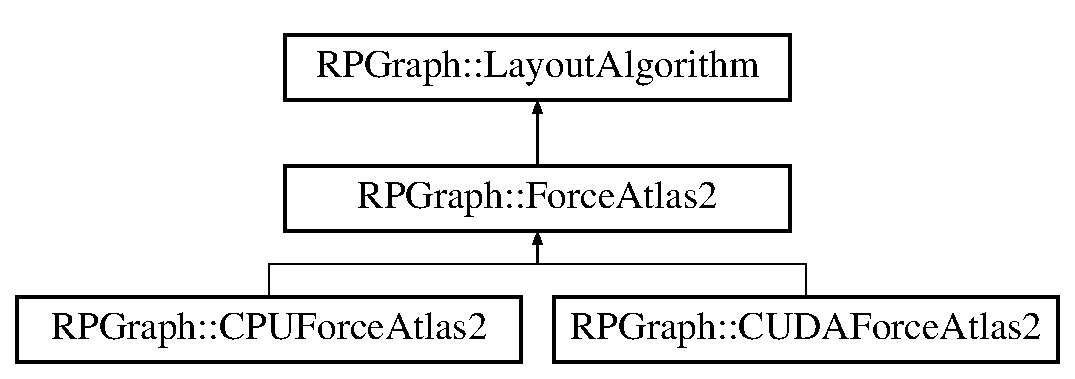
\includegraphics[height=3.000000cm]{classRPGraph_1_1LayoutAlgorithm}
\end{center}
\end{figure}
\subsection*{Public Member Functions}
\begin{DoxyCompactItemize}
\item 
\mbox{\hyperlink{classRPGraph_1_1LayoutAlgorithm_a22686d4c7557f6f2dab0dfce50799b02}{Layout\+Algorithm}} (\mbox{\hyperlink{classRPGraph_1_1GraphLayout}{Graph\+Layout}} \&\mbox{\hyperlink{classRPGraph_1_1LayoutAlgorithm_ac2335a7ccaeb6cef789ea59b99353cf9}{layout}})
\item 
\mbox{\hyperlink{classRPGraph_1_1LayoutAlgorithm_a783dae7e8252ee7e2779aed90850e3d7}{$\sim$\+Layout\+Algorithm}} ()
\item 
virtual void \mbox{\hyperlink{classRPGraph_1_1LayoutAlgorithm_a70f3171d513b92d44f4784ff96c848c1}{sync\+\_\+layout}} ()=0
\end{DoxyCompactItemize}
\subsection*{Public Attributes}
\begin{DoxyCompactItemize}
\item 
\mbox{\hyperlink{classRPGraph_1_1GraphLayout}{Graph\+Layout}} \& \mbox{\hyperlink{classRPGraph_1_1LayoutAlgorithm_ac2335a7ccaeb6cef789ea59b99353cf9}{layout}}
\end{DoxyCompactItemize}


\subsection{Constructor \& Destructor Documentation}
\mbox{\Hypertarget{classRPGraph_1_1LayoutAlgorithm_a22686d4c7557f6f2dab0dfce50799b02}\label{classRPGraph_1_1LayoutAlgorithm_a22686d4c7557f6f2dab0dfce50799b02}} 
\index{R\+P\+Graph\+::\+Layout\+Algorithm@{R\+P\+Graph\+::\+Layout\+Algorithm}!Layout\+Algorithm@{Layout\+Algorithm}}
\index{Layout\+Algorithm@{Layout\+Algorithm}!R\+P\+Graph\+::\+Layout\+Algorithm@{R\+P\+Graph\+::\+Layout\+Algorithm}}
\subsubsection{\texorpdfstring{Layout\+Algorithm()}{LayoutAlgorithm()}}
{\footnotesize\ttfamily R\+P\+Graph\+::\+Layout\+Algorithm\+::\+Layout\+Algorithm (\begin{DoxyParamCaption}\item[{\mbox{\hyperlink{classRPGraph_1_1GraphLayout}{Graph\+Layout}} \&}]{layout }\end{DoxyParamCaption})}

\mbox{\Hypertarget{classRPGraph_1_1LayoutAlgorithm_a783dae7e8252ee7e2779aed90850e3d7}\label{classRPGraph_1_1LayoutAlgorithm_a783dae7e8252ee7e2779aed90850e3d7}} 
\index{R\+P\+Graph\+::\+Layout\+Algorithm@{R\+P\+Graph\+::\+Layout\+Algorithm}!````~Layout\+Algorithm@{$\sim$\+Layout\+Algorithm}}
\index{````~Layout\+Algorithm@{$\sim$\+Layout\+Algorithm}!R\+P\+Graph\+::\+Layout\+Algorithm@{R\+P\+Graph\+::\+Layout\+Algorithm}}
\subsubsection{\texorpdfstring{$\sim$\+Layout\+Algorithm()}{~LayoutAlgorithm()}}
{\footnotesize\ttfamily R\+P\+Graph\+::\+Layout\+Algorithm\+::$\sim$\+Layout\+Algorithm (\begin{DoxyParamCaption}{ }\end{DoxyParamCaption})}



\subsection{Member Function Documentation}
\mbox{\Hypertarget{classRPGraph_1_1LayoutAlgorithm_a70f3171d513b92d44f4784ff96c848c1}\label{classRPGraph_1_1LayoutAlgorithm_a70f3171d513b92d44f4784ff96c848c1}} 
\index{R\+P\+Graph\+::\+Layout\+Algorithm@{R\+P\+Graph\+::\+Layout\+Algorithm}!sync\+\_\+layout@{sync\+\_\+layout}}
\index{sync\+\_\+layout@{sync\+\_\+layout}!R\+P\+Graph\+::\+Layout\+Algorithm@{R\+P\+Graph\+::\+Layout\+Algorithm}}
\subsubsection{\texorpdfstring{sync\+\_\+layout()}{sync\_layout()}}
{\footnotesize\ttfamily virtual void R\+P\+Graph\+::\+Layout\+Algorithm\+::sync\+\_\+layout (\begin{DoxyParamCaption}{ }\end{DoxyParamCaption})\hspace{0.3cm}{\ttfamily [pure virtual]}}



Implemented in \mbox{\hyperlink{classRPGraph_1_1CPUForceAtlas2_afaada68053fce521843af0eb5ca316df}{R\+P\+Graph\+::\+C\+P\+U\+Force\+Atlas2}}, and \mbox{\hyperlink{classRPGraph_1_1CUDAForceAtlas2_a474a1cd717352057859185885b8020cf}{R\+P\+Graph\+::\+C\+U\+D\+A\+Force\+Atlas2}}.



\subsection{Member Data Documentation}
\mbox{\Hypertarget{classRPGraph_1_1LayoutAlgorithm_ac2335a7ccaeb6cef789ea59b99353cf9}\label{classRPGraph_1_1LayoutAlgorithm_ac2335a7ccaeb6cef789ea59b99353cf9}} 
\index{R\+P\+Graph\+::\+Layout\+Algorithm@{R\+P\+Graph\+::\+Layout\+Algorithm}!layout@{layout}}
\index{layout@{layout}!R\+P\+Graph\+::\+Layout\+Algorithm@{R\+P\+Graph\+::\+Layout\+Algorithm}}
\subsubsection{\texorpdfstring{layout}{layout}}
{\footnotesize\ttfamily \mbox{\hyperlink{classRPGraph_1_1GraphLayout}{Graph\+Layout}}\& R\+P\+Graph\+::\+Layout\+Algorithm\+::layout}



The documentation for this class was generated from the following files\+:\begin{DoxyCompactItemize}
\item 
\mbox{\hyperlink{RPLayoutAlgorithm_8hpp}{R\+P\+Layout\+Algorithm.\+hpp}}\item 
\mbox{\hyperlink{RPLayoutAlgorithm_8cpp}{R\+P\+Layout\+Algorithm.\+cpp}}\end{DoxyCompactItemize}

\hypertarget{classRPGraph_1_1Real2DVector}{}\section{R\+P\+Graph\+:\+:Real2\+D\+Vector Class Reference}
\label{classRPGraph_1_1Real2DVector}\index{R\+P\+Graph\+::\+Real2\+D\+Vector@{R\+P\+Graph\+::\+Real2\+D\+Vector}}


{\ttfamily \#include $<$R\+P\+Common.\+hpp$>$}

\subsection*{Public Member Functions}
\begin{DoxyCompactItemize}
\item 
\mbox{\hyperlink{classRPGraph_1_1Real2DVector_af6c81ec0d227c6cd31047e436bf574d5}{Real2\+D\+Vector}} (float \mbox{\hyperlink{classRPGraph_1_1Real2DVector_a4511632e71344b88deee5512b791e97d}{x}}, float \mbox{\hyperlink{classRPGraph_1_1Real2DVector_aa37f96dfb13727fdee7a82ddbd1d7f60}{y}})
\item 
float \mbox{\hyperlink{classRPGraph_1_1Real2DVector_a62125104c62e26ff29b68c190402bdcb}{magnitude}} ()
\item 
float \mbox{\hyperlink{classRPGraph_1_1Real2DVector_ac4f84d862727a3e3c8d31785c8e6a098}{distance}} (\mbox{\hyperlink{classRPGraph_1_1Real2DVector}{Real2\+D\+Vector}} to)
\item 
\mbox{\hyperlink{classRPGraph_1_1Real2DVector}{Real2\+D\+Vector}} \mbox{\hyperlink{classRPGraph_1_1Real2DVector_aed4dbd7713ff8b99da56fa8921d0b7af}{operator$\ast$}} (float b)
\item 
\mbox{\hyperlink{classRPGraph_1_1Real2DVector}{Real2\+D\+Vector}} \mbox{\hyperlink{classRPGraph_1_1Real2DVector_a4517f945dd9656ab21361d9b5d56acd3}{operator/}} (float b)
\item 
\mbox{\hyperlink{classRPGraph_1_1Real2DVector}{Real2\+D\+Vector}} \mbox{\hyperlink{classRPGraph_1_1Real2DVector_a80a9d932a71d70a67041b3881c9927eb}{operator+}} (\mbox{\hyperlink{classRPGraph_1_1Real2DVector}{Real2\+D\+Vector}} b)
\item 
\mbox{\hyperlink{classRPGraph_1_1Real2DVector}{Real2\+D\+Vector}} \mbox{\hyperlink{classRPGraph_1_1Real2DVector_a465750b796cc19dbc290229c2d78d84d}{operator-\/}} (\mbox{\hyperlink{classRPGraph_1_1Real2DVector}{Real2\+D\+Vector}} b)
\item 
void \mbox{\hyperlink{classRPGraph_1_1Real2DVector_a8d1c5fc6b1d4bd683acfa482677ad58a}{operator+=}} (\mbox{\hyperlink{classRPGraph_1_1Real2DVector}{Real2\+D\+Vector}} b)
\item 
\mbox{\hyperlink{classRPGraph_1_1Real2DVector}{Real2\+D\+Vector}} \mbox{\hyperlink{classRPGraph_1_1Real2DVector_a974b46237ab8f38d195061fd9c5b3357}{get\+Normalized}} ()
\item 
\mbox{\hyperlink{classRPGraph_1_1Real2DVector}{Real2\+D\+Vector}} \mbox{\hyperlink{classRPGraph_1_1Real2DVector_ac96e16721ee48ab5fa1ab686c58651f4}{normalize}} ()
\end{DoxyCompactItemize}
\subsection*{Public Attributes}
\begin{DoxyCompactItemize}
\item 
float \mbox{\hyperlink{classRPGraph_1_1Real2DVector_a4511632e71344b88deee5512b791e97d}{x}}
\item 
float \mbox{\hyperlink{classRPGraph_1_1Real2DVector_aa37f96dfb13727fdee7a82ddbd1d7f60}{y}}
\end{DoxyCompactItemize}


\subsection{Constructor \& Destructor Documentation}
\mbox{\Hypertarget{classRPGraph_1_1Real2DVector_af6c81ec0d227c6cd31047e436bf574d5}\label{classRPGraph_1_1Real2DVector_af6c81ec0d227c6cd31047e436bf574d5}} 
\index{R\+P\+Graph\+::\+Real2\+D\+Vector@{R\+P\+Graph\+::\+Real2\+D\+Vector}!Real2\+D\+Vector@{Real2\+D\+Vector}}
\index{Real2\+D\+Vector@{Real2\+D\+Vector}!R\+P\+Graph\+::\+Real2\+D\+Vector@{R\+P\+Graph\+::\+Real2\+D\+Vector}}
\subsubsection{\texorpdfstring{Real2\+D\+Vector()}{Real2DVector()}}
{\footnotesize\ttfamily R\+P\+Graph\+::\+Real2\+D\+Vector\+::\+Real2\+D\+Vector (\begin{DoxyParamCaption}\item[{float}]{x,  }\item[{float}]{y }\end{DoxyParamCaption})}

Why did they have to define their own 2\+D\+Vector class? Usages\+:
\begin{DoxyItemize}
\item R\+P\+Barnes\+Hut\+Approximater
\item R\+P\+C\+P\+U\+Force\+Atlas2
\item R\+P\+Graph\+Layout 
\end{DoxyItemize}

\subsection{Member Function Documentation}
\mbox{\Hypertarget{classRPGraph_1_1Real2DVector_ac4f84d862727a3e3c8d31785c8e6a098}\label{classRPGraph_1_1Real2DVector_ac4f84d862727a3e3c8d31785c8e6a098}} 
\index{R\+P\+Graph\+::\+Real2\+D\+Vector@{R\+P\+Graph\+::\+Real2\+D\+Vector}!distance@{distance}}
\index{distance@{distance}!R\+P\+Graph\+::\+Real2\+D\+Vector@{R\+P\+Graph\+::\+Real2\+D\+Vector}}
\subsubsection{\texorpdfstring{distance()}{distance()}}
{\footnotesize\ttfamily float R\+P\+Graph\+::\+Real2\+D\+Vector\+::distance (\begin{DoxyParamCaption}\item[{\mbox{\hyperlink{classRPGraph_1_1Real2DVector}{R\+P\+Graph\+::\+Real2\+D\+Vector}}}]{to }\end{DoxyParamCaption})}

\mbox{\Hypertarget{classRPGraph_1_1Real2DVector_a974b46237ab8f38d195061fd9c5b3357}\label{classRPGraph_1_1Real2DVector_a974b46237ab8f38d195061fd9c5b3357}} 
\index{R\+P\+Graph\+::\+Real2\+D\+Vector@{R\+P\+Graph\+::\+Real2\+D\+Vector}!get\+Normalized@{get\+Normalized}}
\index{get\+Normalized@{get\+Normalized}!R\+P\+Graph\+::\+Real2\+D\+Vector@{R\+P\+Graph\+::\+Real2\+D\+Vector}}
\subsubsection{\texorpdfstring{get\+Normalized()}{getNormalized()}}
{\footnotesize\ttfamily \mbox{\hyperlink{classRPGraph_1_1Real2DVector}{Real2\+D\+Vector}} R\+P\+Graph\+::\+Real2\+D\+Vector\+::get\+Normalized (\begin{DoxyParamCaption}{ }\end{DoxyParamCaption})}

\mbox{\Hypertarget{classRPGraph_1_1Real2DVector_a62125104c62e26ff29b68c190402bdcb}\label{classRPGraph_1_1Real2DVector_a62125104c62e26ff29b68c190402bdcb}} 
\index{R\+P\+Graph\+::\+Real2\+D\+Vector@{R\+P\+Graph\+::\+Real2\+D\+Vector}!magnitude@{magnitude}}
\index{magnitude@{magnitude}!R\+P\+Graph\+::\+Real2\+D\+Vector@{R\+P\+Graph\+::\+Real2\+D\+Vector}}
\subsubsection{\texorpdfstring{magnitude()}{magnitude()}}
{\footnotesize\ttfamily float R\+P\+Graph\+::\+Real2\+D\+Vector\+::magnitude (\begin{DoxyParamCaption}{ }\end{DoxyParamCaption})}

\mbox{\Hypertarget{classRPGraph_1_1Real2DVector_ac96e16721ee48ab5fa1ab686c58651f4}\label{classRPGraph_1_1Real2DVector_ac96e16721ee48ab5fa1ab686c58651f4}} 
\index{R\+P\+Graph\+::\+Real2\+D\+Vector@{R\+P\+Graph\+::\+Real2\+D\+Vector}!normalize@{normalize}}
\index{normalize@{normalize}!R\+P\+Graph\+::\+Real2\+D\+Vector@{R\+P\+Graph\+::\+Real2\+D\+Vector}}
\subsubsection{\texorpdfstring{normalize()}{normalize()}}
{\footnotesize\ttfamily \mbox{\hyperlink{classRPGraph_1_1Real2DVector}{Real2\+D\+Vector}} R\+P\+Graph\+::\+Real2\+D\+Vector\+::normalize (\begin{DoxyParamCaption}{ }\end{DoxyParamCaption})}

\mbox{\Hypertarget{classRPGraph_1_1Real2DVector_aed4dbd7713ff8b99da56fa8921d0b7af}\label{classRPGraph_1_1Real2DVector_aed4dbd7713ff8b99da56fa8921d0b7af}} 
\index{R\+P\+Graph\+::\+Real2\+D\+Vector@{R\+P\+Graph\+::\+Real2\+D\+Vector}!operator$\ast$@{operator$\ast$}}
\index{operator$\ast$@{operator$\ast$}!R\+P\+Graph\+::\+Real2\+D\+Vector@{R\+P\+Graph\+::\+Real2\+D\+Vector}}
\subsubsection{\texorpdfstring{operator$\ast$()}{operator*()}}
{\footnotesize\ttfamily \mbox{\hyperlink{classRPGraph_1_1Real2DVector}{Real2\+D\+Vector}} R\+P\+Graph\+::\+Real2\+D\+Vector\+::operator$\ast$ (\begin{DoxyParamCaption}\item[{float}]{b }\end{DoxyParamCaption})}

\mbox{\Hypertarget{classRPGraph_1_1Real2DVector_a80a9d932a71d70a67041b3881c9927eb}\label{classRPGraph_1_1Real2DVector_a80a9d932a71d70a67041b3881c9927eb}} 
\index{R\+P\+Graph\+::\+Real2\+D\+Vector@{R\+P\+Graph\+::\+Real2\+D\+Vector}!operator+@{operator+}}
\index{operator+@{operator+}!R\+P\+Graph\+::\+Real2\+D\+Vector@{R\+P\+Graph\+::\+Real2\+D\+Vector}}
\subsubsection{\texorpdfstring{operator+()}{operator+()}}
{\footnotesize\ttfamily \mbox{\hyperlink{classRPGraph_1_1Real2DVector}{Real2\+D\+Vector}} R\+P\+Graph\+::\+Real2\+D\+Vector\+::operator+ (\begin{DoxyParamCaption}\item[{\mbox{\hyperlink{classRPGraph_1_1Real2DVector}{Real2\+D\+Vector}}}]{b }\end{DoxyParamCaption})}

\mbox{\Hypertarget{classRPGraph_1_1Real2DVector_a8d1c5fc6b1d4bd683acfa482677ad58a}\label{classRPGraph_1_1Real2DVector_a8d1c5fc6b1d4bd683acfa482677ad58a}} 
\index{R\+P\+Graph\+::\+Real2\+D\+Vector@{R\+P\+Graph\+::\+Real2\+D\+Vector}!operator+=@{operator+=}}
\index{operator+=@{operator+=}!R\+P\+Graph\+::\+Real2\+D\+Vector@{R\+P\+Graph\+::\+Real2\+D\+Vector}}
\subsubsection{\texorpdfstring{operator+=()}{operator+=()}}
{\footnotesize\ttfamily void R\+P\+Graph\+::\+Real2\+D\+Vector\+::operator+= (\begin{DoxyParamCaption}\item[{\mbox{\hyperlink{classRPGraph_1_1Real2DVector}{Real2\+D\+Vector}}}]{b }\end{DoxyParamCaption})}

\mbox{\Hypertarget{classRPGraph_1_1Real2DVector_a465750b796cc19dbc290229c2d78d84d}\label{classRPGraph_1_1Real2DVector_a465750b796cc19dbc290229c2d78d84d}} 
\index{R\+P\+Graph\+::\+Real2\+D\+Vector@{R\+P\+Graph\+::\+Real2\+D\+Vector}!operator-\/@{operator-\/}}
\index{operator-\/@{operator-\/}!R\+P\+Graph\+::\+Real2\+D\+Vector@{R\+P\+Graph\+::\+Real2\+D\+Vector}}
\subsubsection{\texorpdfstring{operator-\/()}{operator-()}}
{\footnotesize\ttfamily \mbox{\hyperlink{classRPGraph_1_1Real2DVector}{Real2\+D\+Vector}} R\+P\+Graph\+::\+Real2\+D\+Vector\+::operator-\/ (\begin{DoxyParamCaption}\item[{\mbox{\hyperlink{classRPGraph_1_1Real2DVector}{Real2\+D\+Vector}}}]{b }\end{DoxyParamCaption})}

\mbox{\Hypertarget{classRPGraph_1_1Real2DVector_a4517f945dd9656ab21361d9b5d56acd3}\label{classRPGraph_1_1Real2DVector_a4517f945dd9656ab21361d9b5d56acd3}} 
\index{R\+P\+Graph\+::\+Real2\+D\+Vector@{R\+P\+Graph\+::\+Real2\+D\+Vector}!operator/@{operator/}}
\index{operator/@{operator/}!R\+P\+Graph\+::\+Real2\+D\+Vector@{R\+P\+Graph\+::\+Real2\+D\+Vector}}
\subsubsection{\texorpdfstring{operator/()}{operator/()}}
{\footnotesize\ttfamily \mbox{\hyperlink{classRPGraph_1_1Real2DVector}{Real2\+D\+Vector}} R\+P\+Graph\+::\+Real2\+D\+Vector\+::operator/ (\begin{DoxyParamCaption}\item[{float}]{b }\end{DoxyParamCaption})}



\subsection{Member Data Documentation}
\mbox{\Hypertarget{classRPGraph_1_1Real2DVector_a4511632e71344b88deee5512b791e97d}\label{classRPGraph_1_1Real2DVector_a4511632e71344b88deee5512b791e97d}} 
\index{R\+P\+Graph\+::\+Real2\+D\+Vector@{R\+P\+Graph\+::\+Real2\+D\+Vector}!x@{x}}
\index{x@{x}!R\+P\+Graph\+::\+Real2\+D\+Vector@{R\+P\+Graph\+::\+Real2\+D\+Vector}}
\subsubsection{\texorpdfstring{x}{x}}
{\footnotesize\ttfamily float R\+P\+Graph\+::\+Real2\+D\+Vector\+::x}

\mbox{\Hypertarget{classRPGraph_1_1Real2DVector_aa37f96dfb13727fdee7a82ddbd1d7f60}\label{classRPGraph_1_1Real2DVector_aa37f96dfb13727fdee7a82ddbd1d7f60}} 
\index{R\+P\+Graph\+::\+Real2\+D\+Vector@{R\+P\+Graph\+::\+Real2\+D\+Vector}!y@{y}}
\index{y@{y}!R\+P\+Graph\+::\+Real2\+D\+Vector@{R\+P\+Graph\+::\+Real2\+D\+Vector}}
\subsubsection{\texorpdfstring{y}{y}}
{\footnotesize\ttfamily float R\+P\+Graph\+::\+Real2\+D\+Vector\+::y}



The documentation for this class was generated from the following files\+:\begin{DoxyCompactItemize}
\item 
\mbox{\hyperlink{RPCommon_8hpp}{R\+P\+Common.\+hpp}}\item 
\mbox{\hyperlink{RPCommon_8cpp}{R\+P\+Common.\+cpp}}\end{DoxyCompactItemize}

\hypertarget{classRPGraph_1_1UGraph}{}\section{R\+P\+Graph\+:\+:U\+Graph Class Reference}
\label{classRPGraph_1_1UGraph}\index{R\+P\+Graph\+::\+U\+Graph@{R\+P\+Graph\+::\+U\+Graph}}


{\ttfamily \#include $<$R\+P\+Graph.\+hpp$>$}

Inheritance diagram for R\+P\+Graph\+:\+:U\+Graph\+:\begin{figure}[H]
\begin{center}
\leavevmode
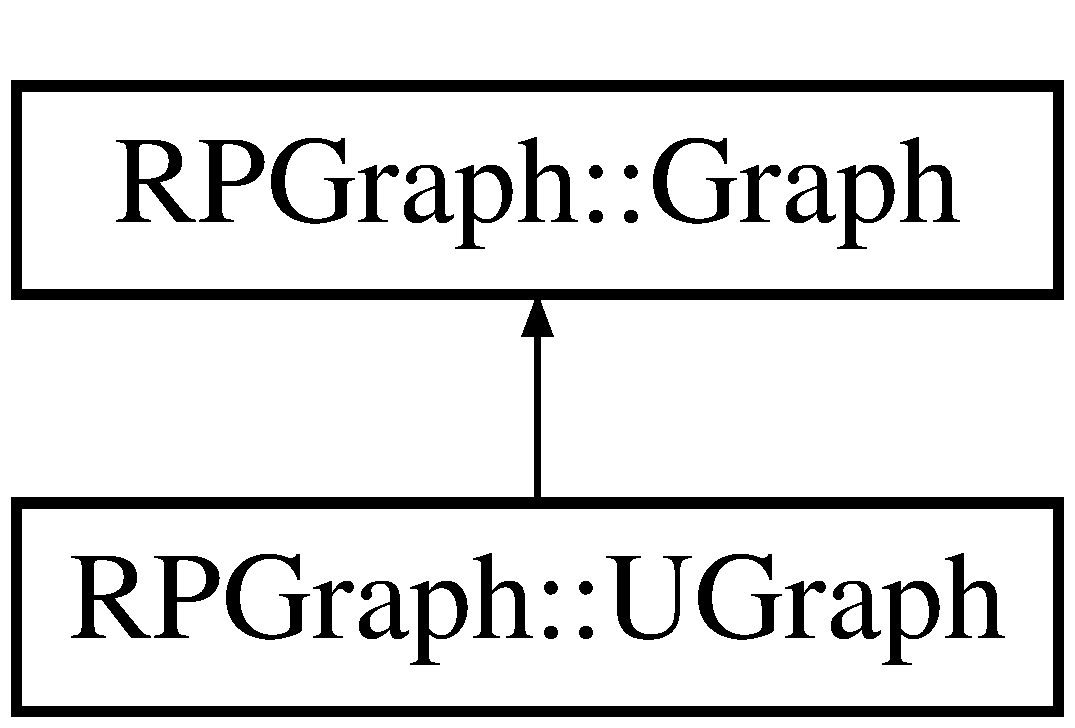
\includegraphics[height=2.000000cm]{classRPGraph_1_1UGraph}
\end{center}
\end{figure}
\subsection*{Public Member Functions}
\begin{DoxyCompactItemize}
\item 
\mbox{\hyperlink{classRPGraph_1_1UGraph_a2e52cd7b17ae1f839b45e26ec6ae1135}{U\+Graph}} (std\+::string edgelist\+\_\+path)
\item 
virtual \mbox{\hyperlink{namespaceRPGraph_ab3ae34f1ab88e48f43794c30c8697b74}{nid\+\_\+t}} \mbox{\hyperlink{classRPGraph_1_1UGraph_ad5eb18fffb7b9a64819b3f1f38305a0c}{num\+\_\+nodes}} () override
\item 
virtual \mbox{\hyperlink{namespaceRPGraph_ab3ae34f1ab88e48f43794c30c8697b74}{nid\+\_\+t}} \mbox{\hyperlink{classRPGraph_1_1UGraph_a55a5deea9a4d456e78e24a2002f31ef2}{num\+\_\+edges}} () override
\item 
virtual \mbox{\hyperlink{namespaceRPGraph_ab3ae34f1ab88e48f43794c30c8697b74}{nid\+\_\+t}} \mbox{\hyperlink{classRPGraph_1_1UGraph_a4d3c3af1ba4787ef5ced5f5efa9d05cf}{degree}} (\mbox{\hyperlink{namespaceRPGraph_ab3ae34f1ab88e48f43794c30c8697b74}{nid\+\_\+t}} nid) override
\item 
virtual \mbox{\hyperlink{namespaceRPGraph_ab3ae34f1ab88e48f43794c30c8697b74}{nid\+\_\+t}} \mbox{\hyperlink{classRPGraph_1_1UGraph_a5614092aab1bb8d92b625506f944d39c}{in\+\_\+degree}} (\mbox{\hyperlink{namespaceRPGraph_ab3ae34f1ab88e48f43794c30c8697b74}{nid\+\_\+t}} nid) override
\item 
virtual \mbox{\hyperlink{namespaceRPGraph_ab3ae34f1ab88e48f43794c30c8697b74}{nid\+\_\+t}} \mbox{\hyperlink{classRPGraph_1_1UGraph_a8416a5fa8b87b8569d0fa563288ac162}{out\+\_\+degree}} (\mbox{\hyperlink{namespaceRPGraph_ab3ae34f1ab88e48f43794c30c8697b74}{nid\+\_\+t}} nid) override
\item 
std\+::vector$<$ \mbox{\hyperlink{namespaceRPGraph_ab3ae34f1ab88e48f43794c30c8697b74}{nid\+\_\+t}} $>$ \mbox{\hyperlink{classRPGraph_1_1UGraph_a8cc5be5cfd41f351d4f98de816028f90}{neighbors\+\_\+with\+\_\+geq\+\_\+id}} (\mbox{\hyperlink{namespaceRPGraph_ab3ae34f1ab88e48f43794c30c8697b74}{nid\+\_\+t}} nid) override
\end{DoxyCompactItemize}
\subsection*{Public Attributes}
\begin{DoxyCompactItemize}
\item 
std\+::unordered\+\_\+map$<$ \mbox{\hyperlink{namespaceRPGraph_ab3ae34f1ab88e48f43794c30c8697b74}{nid\+\_\+t}}, \mbox{\hyperlink{namespaceRPGraph_ab3ae34f1ab88e48f43794c30c8697b74}{nid\+\_\+t}} $>$ \mbox{\hyperlink{classRPGraph_1_1UGraph_a084f2f04bcf93eb362fbf1d275a1c018}{node\+\_\+map}}
\item 
std\+::unordered\+\_\+map$<$ \mbox{\hyperlink{namespaceRPGraph_ab3ae34f1ab88e48f43794c30c8697b74}{nid\+\_\+t}}, \mbox{\hyperlink{namespaceRPGraph_ab3ae34f1ab88e48f43794c30c8697b74}{nid\+\_\+t}} $>$ \mbox{\hyperlink{classRPGraph_1_1UGraph_a688250d7d12a6a901325a4ee7b3b518d}{node\+\_\+map\+\_\+r}}
\end{DoxyCompactItemize}


\subsection{Constructor \& Destructor Documentation}
\mbox{\Hypertarget{classRPGraph_1_1UGraph_a2e52cd7b17ae1f839b45e26ec6ae1135}\label{classRPGraph_1_1UGraph_a2e52cd7b17ae1f839b45e26ec6ae1135}} 
\index{R\+P\+Graph\+::\+U\+Graph@{R\+P\+Graph\+::\+U\+Graph}!U\+Graph@{U\+Graph}}
\index{U\+Graph@{U\+Graph}!R\+P\+Graph\+::\+U\+Graph@{R\+P\+Graph\+::\+U\+Graph}}
\subsubsection{\texorpdfstring{U\+Graph()}{UGraph()}}
{\footnotesize\ttfamily R\+P\+Graph\+::\+U\+Graph\+::\+U\+Graph (\begin{DoxyParamCaption}\item[{std\+::string}]{edgelist\+\_\+path }\end{DoxyParamCaption})}

Used once in main file (\mbox{\hyperlink{graph__viewer_8cpp}{graph\+\_\+viewer.\+cpp}}) 

\subsection{Member Function Documentation}
\mbox{\Hypertarget{classRPGraph_1_1UGraph_a4d3c3af1ba4787ef5ced5f5efa9d05cf}\label{classRPGraph_1_1UGraph_a4d3c3af1ba4787ef5ced5f5efa9d05cf}} 
\index{R\+P\+Graph\+::\+U\+Graph@{R\+P\+Graph\+::\+U\+Graph}!degree@{degree}}
\index{degree@{degree}!R\+P\+Graph\+::\+U\+Graph@{R\+P\+Graph\+::\+U\+Graph}}
\subsubsection{\texorpdfstring{degree()}{degree()}}
{\footnotesize\ttfamily \mbox{\hyperlink{namespaceRPGraph_ab3ae34f1ab88e48f43794c30c8697b74}{nid\+\_\+t}} R\+P\+Graph\+::\+U\+Graph\+::degree (\begin{DoxyParamCaption}\item[{\mbox{\hyperlink{namespaceRPGraph_ab3ae34f1ab88e48f43794c30c8697b74}{nid\+\_\+t}}}]{nid }\end{DoxyParamCaption})\hspace{0.3cm}{\ttfamily [override]}, {\ttfamily [virtual]}}



Implements \mbox{\hyperlink{classRPGraph_1_1Graph_a8a95d1f403c3d9860cf7399abc820c7d}{R\+P\+Graph\+::\+Graph}}.

\mbox{\Hypertarget{classRPGraph_1_1UGraph_a5614092aab1bb8d92b625506f944d39c}\label{classRPGraph_1_1UGraph_a5614092aab1bb8d92b625506f944d39c}} 
\index{R\+P\+Graph\+::\+U\+Graph@{R\+P\+Graph\+::\+U\+Graph}!in\+\_\+degree@{in\+\_\+degree}}
\index{in\+\_\+degree@{in\+\_\+degree}!R\+P\+Graph\+::\+U\+Graph@{R\+P\+Graph\+::\+U\+Graph}}
\subsubsection{\texorpdfstring{in\+\_\+degree()}{in\_degree()}}
{\footnotesize\ttfamily \mbox{\hyperlink{namespaceRPGraph_ab3ae34f1ab88e48f43794c30c8697b74}{nid\+\_\+t}} R\+P\+Graph\+::\+U\+Graph\+::in\+\_\+degree (\begin{DoxyParamCaption}\item[{\mbox{\hyperlink{namespaceRPGraph_ab3ae34f1ab88e48f43794c30c8697b74}{nid\+\_\+t}}}]{nid }\end{DoxyParamCaption})\hspace{0.3cm}{\ttfamily [override]}, {\ttfamily [virtual]}}



Implements \mbox{\hyperlink{classRPGraph_1_1Graph_ab75e19f698a4ab99e37593c7178f2c1a}{R\+P\+Graph\+::\+Graph}}.

\mbox{\Hypertarget{classRPGraph_1_1UGraph_a8cc5be5cfd41f351d4f98de816028f90}\label{classRPGraph_1_1UGraph_a8cc5be5cfd41f351d4f98de816028f90}} 
\index{R\+P\+Graph\+::\+U\+Graph@{R\+P\+Graph\+::\+U\+Graph}!neighbors\+\_\+with\+\_\+geq\+\_\+id@{neighbors\+\_\+with\+\_\+geq\+\_\+id}}
\index{neighbors\+\_\+with\+\_\+geq\+\_\+id@{neighbors\+\_\+with\+\_\+geq\+\_\+id}!R\+P\+Graph\+::\+U\+Graph@{R\+P\+Graph\+::\+U\+Graph}}
\subsubsection{\texorpdfstring{neighbors\+\_\+with\+\_\+geq\+\_\+id()}{neighbors\_with\_geq\_id()}}
{\footnotesize\ttfamily std\+::vector$<$ \mbox{\hyperlink{namespaceRPGraph_ab3ae34f1ab88e48f43794c30c8697b74}{nid\+\_\+t}} $>$ R\+P\+Graph\+::\+U\+Graph\+::neighbors\+\_\+with\+\_\+geq\+\_\+id (\begin{DoxyParamCaption}\item[{\mbox{\hyperlink{namespaceRPGraph_ab3ae34f1ab88e48f43794c30c8697b74}{nid\+\_\+t}}}]{nid }\end{DoxyParamCaption})\hspace{0.3cm}{\ttfamily [override]}, {\ttfamily [virtual]}}



Implements \mbox{\hyperlink{classRPGraph_1_1Graph_ab1e27e4268d36443a5db035fa7635cad}{R\+P\+Graph\+::\+Graph}}.

\mbox{\Hypertarget{classRPGraph_1_1UGraph_a55a5deea9a4d456e78e24a2002f31ef2}\label{classRPGraph_1_1UGraph_a55a5deea9a4d456e78e24a2002f31ef2}} 
\index{R\+P\+Graph\+::\+U\+Graph@{R\+P\+Graph\+::\+U\+Graph}!num\+\_\+edges@{num\+\_\+edges}}
\index{num\+\_\+edges@{num\+\_\+edges}!R\+P\+Graph\+::\+U\+Graph@{R\+P\+Graph\+::\+U\+Graph}}
\subsubsection{\texorpdfstring{num\+\_\+edges()}{num\_edges()}}
{\footnotesize\ttfamily \mbox{\hyperlink{namespaceRPGraph_ab3ae34f1ab88e48f43794c30c8697b74}{nid\+\_\+t}} R\+P\+Graph\+::\+U\+Graph\+::num\+\_\+edges (\begin{DoxyParamCaption}{ }\end{DoxyParamCaption})\hspace{0.3cm}{\ttfamily [override]}, {\ttfamily [virtual]}}



Implements \mbox{\hyperlink{classRPGraph_1_1Graph_acd3b877216686aff2f7fbc2d62bcdf9b}{R\+P\+Graph\+::\+Graph}}.

\mbox{\Hypertarget{classRPGraph_1_1UGraph_ad5eb18fffb7b9a64819b3f1f38305a0c}\label{classRPGraph_1_1UGraph_ad5eb18fffb7b9a64819b3f1f38305a0c}} 
\index{R\+P\+Graph\+::\+U\+Graph@{R\+P\+Graph\+::\+U\+Graph}!num\+\_\+nodes@{num\+\_\+nodes}}
\index{num\+\_\+nodes@{num\+\_\+nodes}!R\+P\+Graph\+::\+U\+Graph@{R\+P\+Graph\+::\+U\+Graph}}
\subsubsection{\texorpdfstring{num\+\_\+nodes()}{num\_nodes()}}
{\footnotesize\ttfamily \mbox{\hyperlink{namespaceRPGraph_ab3ae34f1ab88e48f43794c30c8697b74}{nid\+\_\+t}} R\+P\+Graph\+::\+U\+Graph\+::num\+\_\+nodes (\begin{DoxyParamCaption}{ }\end{DoxyParamCaption})\hspace{0.3cm}{\ttfamily [override]}, {\ttfamily [virtual]}}



Implements \mbox{\hyperlink{classRPGraph_1_1Graph_ab5602e6b776a0ea3b944775331fcb2aa}{R\+P\+Graph\+::\+Graph}}.

\mbox{\Hypertarget{classRPGraph_1_1UGraph_a8416a5fa8b87b8569d0fa563288ac162}\label{classRPGraph_1_1UGraph_a8416a5fa8b87b8569d0fa563288ac162}} 
\index{R\+P\+Graph\+::\+U\+Graph@{R\+P\+Graph\+::\+U\+Graph}!out\+\_\+degree@{out\+\_\+degree}}
\index{out\+\_\+degree@{out\+\_\+degree}!R\+P\+Graph\+::\+U\+Graph@{R\+P\+Graph\+::\+U\+Graph}}
\subsubsection{\texorpdfstring{out\+\_\+degree()}{out\_degree()}}
{\footnotesize\ttfamily \mbox{\hyperlink{namespaceRPGraph_ab3ae34f1ab88e48f43794c30c8697b74}{nid\+\_\+t}} R\+P\+Graph\+::\+U\+Graph\+::out\+\_\+degree (\begin{DoxyParamCaption}\item[{\mbox{\hyperlink{namespaceRPGraph_ab3ae34f1ab88e48f43794c30c8697b74}{nid\+\_\+t}}}]{nid }\end{DoxyParamCaption})\hspace{0.3cm}{\ttfamily [override]}, {\ttfamily [virtual]}}



Implements \mbox{\hyperlink{classRPGraph_1_1Graph_a660ad58e03df7e3cc00d0eb4e5c16819}{R\+P\+Graph\+::\+Graph}}.



\subsection{Member Data Documentation}
\mbox{\Hypertarget{classRPGraph_1_1UGraph_a084f2f04bcf93eb362fbf1d275a1c018}\label{classRPGraph_1_1UGraph_a084f2f04bcf93eb362fbf1d275a1c018}} 
\index{R\+P\+Graph\+::\+U\+Graph@{R\+P\+Graph\+::\+U\+Graph}!node\+\_\+map@{node\+\_\+map}}
\index{node\+\_\+map@{node\+\_\+map}!R\+P\+Graph\+::\+U\+Graph@{R\+P\+Graph\+::\+U\+Graph}}
\subsubsection{\texorpdfstring{node\+\_\+map}{node\_map}}
{\footnotesize\ttfamily std\+::unordered\+\_\+map$<$\mbox{\hyperlink{namespaceRPGraph_ab3ae34f1ab88e48f43794c30c8697b74}{nid\+\_\+t}}, \mbox{\hyperlink{namespaceRPGraph_ab3ae34f1ab88e48f43794c30c8697b74}{nid\+\_\+t}}$>$ R\+P\+Graph\+::\+U\+Graph\+::node\+\_\+map}

\mbox{\Hypertarget{classRPGraph_1_1UGraph_a688250d7d12a6a901325a4ee7b3b518d}\label{classRPGraph_1_1UGraph_a688250d7d12a6a901325a4ee7b3b518d}} 
\index{R\+P\+Graph\+::\+U\+Graph@{R\+P\+Graph\+::\+U\+Graph}!node\+\_\+map\+\_\+r@{node\+\_\+map\+\_\+r}}
\index{node\+\_\+map\+\_\+r@{node\+\_\+map\+\_\+r}!R\+P\+Graph\+::\+U\+Graph@{R\+P\+Graph\+::\+U\+Graph}}
\subsubsection{\texorpdfstring{node\+\_\+map\+\_\+r}{node\_map\_r}}
{\footnotesize\ttfamily std\+::unordered\+\_\+map$<$\mbox{\hyperlink{namespaceRPGraph_ab3ae34f1ab88e48f43794c30c8697b74}{nid\+\_\+t}}, \mbox{\hyperlink{namespaceRPGraph_ab3ae34f1ab88e48f43794c30c8697b74}{nid\+\_\+t}}$>$ R\+P\+Graph\+::\+U\+Graph\+::node\+\_\+map\+\_\+r}



The documentation for this class was generated from the following files\+:\begin{DoxyCompactItemize}
\item 
\mbox{\hyperlink{RPGraph_8hpp}{R\+P\+Graph.\+hpp}}\item 
\mbox{\hyperlink{RPGraph_8cpp}{R\+P\+Graph.\+cpp}}\end{DoxyCompactItemize}

\chapter{File Documentation}
\hypertarget{graph__viewer_8cpp}{}\section{graph\+\_\+viewer.\+cpp File Reference}
\label{graph__viewer_8cpp}\index{graph\+\_\+viewer.\+cpp@{graph\+\_\+viewer.\+cpp}}
{\ttfamily \#include $<$stdio.\+h$>$}\newline
{\ttfamily \#include $<$stdlib.\+h$>$}\newline
{\ttfamily \#include $<$string$>$}\newline
{\ttfamily \#include $<$math.\+h$>$}\newline
{\ttfamily \#include \char`\"{}R\+P\+Common.\+hpp\char`\"{}}\newline
{\ttfamily \#include \char`\"{}R\+P\+Graph.\+hpp\char`\"{}}\newline
{\ttfamily \#include \char`\"{}R\+P\+Graph\+Layout.\+hpp\char`\"{}}\newline
{\ttfamily \#include \char`\"{}R\+P\+C\+P\+U\+Force\+Atlas2.\+hpp\char`\"{}}\newline
\subsection*{Functions}
\begin{DoxyCompactItemize}
\item 
int \mbox{\hyperlink{graph__viewer_8cpp_a217dbf8b442f20279ea00b898af96f52}{main}} (int argc, const char $\ast$$\ast$argv)
\end{DoxyCompactItemize}


\subsection{Function Documentation}
\mbox{\Hypertarget{graph__viewer_8cpp_a217dbf8b442f20279ea00b898af96f52}\label{graph__viewer_8cpp_a217dbf8b442f20279ea00b898af96f52}} 
\index{graph\+\_\+viewer.\+cpp@{graph\+\_\+viewer.\+cpp}!main@{main}}
\index{main@{main}!graph\+\_\+viewer.\+cpp@{graph\+\_\+viewer.\+cpp}}
\subsubsection{\texorpdfstring{main()}{main()}}
{\footnotesize\ttfamily int main (\begin{DoxyParamCaption}\item[{int}]{argc,  }\item[{const char $\ast$$\ast$}]{argv }\end{DoxyParamCaption})}

Entry point for executable. C\+PU or G\+PU. U\+Graph object of adjaceny list format.

T\+O\+DO\+: Wrap this in a function and use it twice, once for the comm layout and once for the full layout.

Implementation in either R\+P\+G\+P\+U\+Force\+Atlas2.\+cpp or \mbox{\hyperlink{RPCPUForceAtlas2_8cpp}{R\+P\+C\+P\+U\+Force\+Atlas2.\+cpp}}

Reverted to older version after multiple issues with the line intended to extract the basename of the network
\hypertarget{read__files_8md}{}\section{read\+\_\+files.\+md File Reference}
\label{read__files_8md}\index{read\+\_\+files.\+md@{read\+\_\+files.\+md}}

\hypertarget{RPBarnesHutApproximator_8cpp}{}\section{R\+P\+Barnes\+Hut\+Approximator.\+cpp File Reference}
\label{RPBarnesHutApproximator_8cpp}\index{R\+P\+Barnes\+Hut\+Approximator.\+cpp@{R\+P\+Barnes\+Hut\+Approximator.\+cpp}}
{\ttfamily \#include \char`\"{}R\+P\+Barnes\+Hut\+Approximator.\+hpp\char`\"{}}\newline
{\ttfamily \#include $<$math.\+h$>$}\newline
{\ttfamily \#include $<$stdlib.\+h$>$}\newline
{\ttfamily \#include $<$queue$>$}\newline
\subsection*{Namespaces}
\begin{DoxyCompactItemize}
\item 
 \mbox{\hyperlink{namespaceRPGraph}{R\+P\+Graph}}
\end{DoxyCompactItemize}

\hypertarget{RPBarnesHutApproximator_8hpp}{}\section{R\+P\+Barnes\+Hut\+Approximator.\+hpp File Reference}
\label{RPBarnesHutApproximator_8hpp}\index{R\+P\+Barnes\+Hut\+Approximator.\+hpp@{R\+P\+Barnes\+Hut\+Approximator.\+hpp}}
{\ttfamily \#include \char`\"{}R\+P\+Graph.\+hpp\char`\"{}}\newline
{\ttfamily \#include \char`\"{}R\+P\+Common.\+hpp\char`\"{}}\newline
\subsection*{Classes}
\begin{DoxyCompactItemize}
\item 
class \mbox{\hyperlink{classRPGraph_1_1BarnesHutCell}{R\+P\+Graph\+::\+Barnes\+Hut\+Cell}}
\item 
class \mbox{\hyperlink{classRPGraph_1_1BarnesHutApproximator}{R\+P\+Graph\+::\+Barnes\+Hut\+Approximator}}
\end{DoxyCompactItemize}
\subsection*{Namespaces}
\begin{DoxyCompactItemize}
\item 
 \mbox{\hyperlink{namespaceRPGraph}{R\+P\+Graph}}
\end{DoxyCompactItemize}

\hypertarget{RPCommon_8cpp}{}\section{R\+P\+Common.\+cpp File Reference}
\label{RPCommon_8cpp}\index{R\+P\+Common.\+cpp@{R\+P\+Common.\+cpp}}
{\ttfamily \#include \char`\"{}R\+P\+Common.\+hpp\char`\"{}}\newline
{\ttfamily \#include $<$stdlib.\+h$>$}\newline
{\ttfamily \#include $<$cmath$>$}\newline
{\ttfamily \#include $<$fstream$>$}\newline
\subsection*{Namespaces}
\begin{DoxyCompactItemize}
\item 
 \mbox{\hyperlink{namespaceRPGraph}{R\+P\+Graph}}
\end{DoxyCompactItemize}
\subsection*{Functions}
\begin{DoxyCompactItemize}
\item 
bool \mbox{\hyperlink{RPCommon_8cpp_a041136f61c39ba0f88d18e72542c6eba}{is\+\_\+file\+\_\+exists}} (const char $\ast$filename)
\item 
float \mbox{\hyperlink{namespaceRPGraph_af65dfa4ca7a18662d86db71341a4478d}{R\+P\+Graph\+::get\+\_\+random}} (float lowerbound, float upperbound)
\item 
float \mbox{\hyperlink{namespaceRPGraph_ac0ea5eed59279f669d6a944798a58d48}{R\+P\+Graph\+::distance}} (Coordinate from, Coordinate to)
\item 
float \mbox{\hyperlink{namespaceRPGraph_aa54d04cd9574e91651e2566eb868df1f}{R\+P\+Graph\+::distance2}} (Coordinate from, Coordinate to)
\item 
Real2\+D\+Vector \mbox{\hyperlink{namespaceRPGraph_ab7f99412b5c91ab02e4a74885a49e9a6}{R\+P\+Graph\+::normalized\+Direction}} (Coordinate from, Coordinate to)
\item 
Real2\+D\+Vector \mbox{\hyperlink{namespaceRPGraph_a18f01f18cedd3449b2bface612bde934}{R\+P\+Graph\+::direction}} (Coordinate from, Coordinate to)
\end{DoxyCompactItemize}


\subsection{Function Documentation}
\mbox{\Hypertarget{RPCommon_8cpp_a041136f61c39ba0f88d18e72542c6eba}\label{RPCommon_8cpp_a041136f61c39ba0f88d18e72542c6eba}} 
\index{R\+P\+Common.\+cpp@{R\+P\+Common.\+cpp}!is\+\_\+file\+\_\+exists@{is\+\_\+file\+\_\+exists}}
\index{is\+\_\+file\+\_\+exists@{is\+\_\+file\+\_\+exists}!R\+P\+Common.\+cpp@{R\+P\+Common.\+cpp}}
\subsubsection{\texorpdfstring{is\+\_\+file\+\_\+exists()}{is\_file\_exists()}}
{\footnotesize\ttfamily bool is\+\_\+file\+\_\+exists (\begin{DoxyParamCaption}\item[{const char $\ast$}]{filename }\end{DoxyParamCaption})}


\hypertarget{RPCommon_8hpp}{}\section{R\+P\+Common.\+hpp File Reference}
\label{RPCommon_8hpp}\index{R\+P\+Common.\+hpp@{R\+P\+Common.\+hpp}}
\subsection*{Classes}
\begin{DoxyCompactItemize}
\item 
class \mbox{\hyperlink{classRPGraph_1_1Real2DVector}{R\+P\+Graph\+::\+Real2\+D\+Vector}}
\item 
class \mbox{\hyperlink{classRPGraph_1_1Coordinate}{R\+P\+Graph\+::\+Coordinate}}
\end{DoxyCompactItemize}
\subsection*{Namespaces}
\begin{DoxyCompactItemize}
\item 
 \mbox{\hyperlink{namespaceRPGraph}{R\+P\+Graph}}
\end{DoxyCompactItemize}
\subsection*{Functions}
\begin{DoxyCompactItemize}
\item 
bool \mbox{\hyperlink{RPCommon_8hpp_a041136f61c39ba0f88d18e72542c6eba}{is\+\_\+file\+\_\+exists}} (const char $\ast$filename)
\item 
float \mbox{\hyperlink{namespaceRPGraph_af65dfa4ca7a18662d86db71341a4478d}{R\+P\+Graph\+::get\+\_\+random}} (float lowerbound, float upperbound)
\item 
float \mbox{\hyperlink{namespaceRPGraph_ac0ea5eed59279f669d6a944798a58d48}{R\+P\+Graph\+::distance}} (Coordinate from, Coordinate to)
\item 
float \mbox{\hyperlink{namespaceRPGraph_aa54d04cd9574e91651e2566eb868df1f}{R\+P\+Graph\+::distance2}} (Coordinate from, Coordinate to)
\item 
Real2\+D\+Vector \mbox{\hyperlink{namespaceRPGraph_ab7f99412b5c91ab02e4a74885a49e9a6}{R\+P\+Graph\+::normalized\+Direction}} (Coordinate from, Coordinate to)
\item 
Real2\+D\+Vector \mbox{\hyperlink{namespaceRPGraph_a18f01f18cedd3449b2bface612bde934}{R\+P\+Graph\+::direction}} (Coordinate from, Coordinate to)
\end{DoxyCompactItemize}


\subsection{Function Documentation}
\mbox{\Hypertarget{RPCommon_8hpp_a041136f61c39ba0f88d18e72542c6eba}\label{RPCommon_8hpp_a041136f61c39ba0f88d18e72542c6eba}} 
\index{R\+P\+Common.\+hpp@{R\+P\+Common.\+hpp}!is\+\_\+file\+\_\+exists@{is\+\_\+file\+\_\+exists}}
\index{is\+\_\+file\+\_\+exists@{is\+\_\+file\+\_\+exists}!R\+P\+Common.\+hpp@{R\+P\+Common.\+hpp}}
\subsubsection{\texorpdfstring{is\+\_\+file\+\_\+exists()}{is\_file\_exists()}}
{\footnotesize\ttfamily bool is\+\_\+file\+\_\+exists (\begin{DoxyParamCaption}\item[{const char $\ast$}]{filename }\end{DoxyParamCaption})}


\hypertarget{RPCPUForceAtlas2_8cpp}{}\section{R\+P\+C\+P\+U\+Force\+Atlas2.\+cpp File Reference}
\label{RPCPUForceAtlas2_8cpp}\index{R\+P\+C\+P\+U\+Force\+Atlas2.\+cpp@{R\+P\+C\+P\+U\+Force\+Atlas2.\+cpp}}
{\ttfamily \#include \char`\"{}R\+P\+C\+P\+U\+Force\+Atlas2.\+hpp\char`\"{}}\newline
{\ttfamily \#include $<$stdlib.\+h$>$}\newline
{\ttfamily \#include $<$math.\+h$>$}\newline
{\ttfamily \#include $<$limits$>$}\newline
{\ttfamily \#include $<$cmath$>$}\newline
{\ttfamily \#include $<$chrono$>$}\newline
\subsection*{Namespaces}
\begin{DoxyCompactItemize}
\item 
 \mbox{\hyperlink{namespaceRPGraph}{R\+P\+Graph}}
\end{DoxyCompactItemize}

\hypertarget{RPCPUForceAtlas2_8hpp}{}\section{R\+P\+C\+P\+U\+Force\+Atlas2.\+hpp File Reference}
\label{RPCPUForceAtlas2_8hpp}\index{R\+P\+C\+P\+U\+Force\+Atlas2.\+hpp@{R\+P\+C\+P\+U\+Force\+Atlas2.\+hpp}}
{\ttfamily \#include \char`\"{}R\+P\+Force\+Atlas2.\+hpp\char`\"{}}\newline
\subsection*{Classes}
\begin{DoxyCompactItemize}
\item 
class \mbox{\hyperlink{classRPGraph_1_1CPUForceAtlas2}{R\+P\+Graph\+::\+C\+P\+U\+Force\+Atlas2}}
\end{DoxyCompactItemize}
\subsection*{Namespaces}
\begin{DoxyCompactItemize}
\item 
 \mbox{\hyperlink{namespaceRPGraph}{R\+P\+Graph}}
\end{DoxyCompactItemize}

\hypertarget{RPForceAtlas2_8cpp}{}\section{R\+P\+Force\+Atlas2.\+cpp File Reference}
\label{RPForceAtlas2_8cpp}\index{R\+P\+Force\+Atlas2.\+cpp@{R\+P\+Force\+Atlas2.\+cpp}}
{\ttfamily \#include \char`\"{}R\+P\+Force\+Atlas2.\+hpp\char`\"{}}\newline
\subsection*{Namespaces}
\begin{DoxyCompactItemize}
\item 
 \mbox{\hyperlink{namespaceRPGraph}{R\+P\+Graph}}
\end{DoxyCompactItemize}

\hypertarget{RPForceAtlas2_8hpp}{}\section{R\+P\+Force\+Atlas2.\+hpp File Reference}
\label{RPForceAtlas2_8hpp}\index{R\+P\+Force\+Atlas2.\+hpp@{R\+P\+Force\+Atlas2.\+hpp}}
{\ttfamily \#include \char`\"{}R\+P\+Layout\+Algorithm.\+hpp\char`\"{}}\newline
{\ttfamily \#include \char`\"{}R\+P\+Barnes\+Hut\+Approximator.\+hpp\char`\"{}}\newline
\subsection*{Classes}
\begin{DoxyCompactItemize}
\item 
class \mbox{\hyperlink{classRPGraph_1_1ForceAtlas2}{R\+P\+Graph\+::\+Force\+Atlas2}}
\end{DoxyCompactItemize}
\subsection*{Namespaces}
\begin{DoxyCompactItemize}
\item 
 \mbox{\hyperlink{namespaceRPGraph}{R\+P\+Graph}}
\end{DoxyCompactItemize}

\hypertarget{RPGPUForceAtlas2_8hpp}{}\section{R\+P\+G\+P\+U\+Force\+Atlas2.\+hpp File Reference}
\label{RPGPUForceAtlas2_8hpp}\index{R\+P\+G\+P\+U\+Force\+Atlas2.\+hpp@{R\+P\+G\+P\+U\+Force\+Atlas2.\+hpp}}
{\ttfamily \#include \char`\"{}R\+P\+Force\+Atlas2.\+hpp\char`\"{}}\newline
\subsection*{Classes}
\begin{DoxyCompactItemize}
\item 
class \mbox{\hyperlink{classRPGraph_1_1CUDAForceAtlas2}{R\+P\+Graph\+::\+C\+U\+D\+A\+Force\+Atlas2}}
\end{DoxyCompactItemize}
\subsection*{Namespaces}
\begin{DoxyCompactItemize}
\item 
 \mbox{\hyperlink{namespaceRPGraph}{R\+P\+Graph}}
\end{DoxyCompactItemize}

\hypertarget{RPGraph_8cpp}{}\section{R\+P\+Graph.\+cpp File Reference}
\label{RPGraph_8cpp}\index{R\+P\+Graph.\+cpp@{R\+P\+Graph.\+cpp}}
{\ttfamily \#include $<$stdio.\+h$>$}\newline
{\ttfamily \#include $<$stdlib.\+h$>$}\newline
{\ttfamily \#include $<$sstream$>$}\newline
{\ttfamily \#include $<$fstream$>$}\newline
{\ttfamily \#include $<$algorithm$>$}\newline
{\ttfamily \#include \char`\"{}R\+P\+Graph.\+hpp\char`\"{}}\newline
\subsection*{Namespaces}
\begin{DoxyCompactItemize}
\item 
 \mbox{\hyperlink{namespaceRPGraph}{R\+P\+Graph}}
\end{DoxyCompactItemize}

\hypertarget{RPGraph_8hpp}{}\section{R\+P\+Graph.\+hpp File Reference}
\label{RPGraph_8hpp}\index{R\+P\+Graph.\+hpp@{R\+P\+Graph.\+hpp}}
{\ttfamily \#include $<$vector$>$}\newline
{\ttfamily \#include $<$string$>$}\newline
{\ttfamily \#include $<$unordered\+\_\+map$>$}\newline
\subsection*{Classes}
\begin{DoxyCompactItemize}
\item 
class \mbox{\hyperlink{classRPGraph_1_1Graph}{R\+P\+Graph\+::\+Graph}}
\item 
class \mbox{\hyperlink{classRPGraph_1_1UGraph}{R\+P\+Graph\+::\+U\+Graph}}
\item 
class \mbox{\hyperlink{classRPGraph_1_1CSRUGraph}{R\+P\+Graph\+::\+C\+S\+R\+U\+Graph}}
\end{DoxyCompactItemize}
\subsection*{Namespaces}
\begin{DoxyCompactItemize}
\item 
 \mbox{\hyperlink{namespaceRPGraph}{R\+P\+Graph}}
\end{DoxyCompactItemize}
\subsection*{Typedefs}
\begin{DoxyCompactItemize}
\item 
typedef uint32\+\_\+t \mbox{\hyperlink{namespaceRPGraph_ab3ae34f1ab88e48f43794c30c8697b74}{R\+P\+Graph\+::nid\+\_\+t}}
\item 
typedef uint32\+\_\+t \mbox{\hyperlink{namespaceRPGraph_ae1c8374fd31c97d09000581a63811ee4}{R\+P\+Graph\+::eid\+\_\+t}}
\end{DoxyCompactItemize}

\hypertarget{RPGraphLayout_8cpp}{}\section{R\+P\+Graph\+Layout.\+cpp File Reference}
\label{RPGraphLayout_8cpp}\index{R\+P\+Graph\+Layout.\+cpp@{R\+P\+Graph\+Layout.\+cpp}}
{\ttfamily \#include \char`\"{}R\+P\+Graph\+Layout.\+hpp\char`\"{}}\newline
{\ttfamily \#include \char`\"{}../lib/pngwriter/src/pngwriter.\+h\char`\"{}}\newline
{\ttfamily \#include $<$fstream$>$}\newline
{\ttfamily \#include $<$limits$>$}\newline
\subsection*{Namespaces}
\begin{DoxyCompactItemize}
\item 
 \mbox{\hyperlink{namespaceRPGraph}{R\+P\+Graph}}
\end{DoxyCompactItemize}

\hypertarget{RPGraphLayout_8hpp}{}\section{R\+P\+Graph\+Layout.\+hpp File Reference}
\label{RPGraphLayout_8hpp}\index{R\+P\+Graph\+Layout.\+hpp@{R\+P\+Graph\+Layout.\+hpp}}
{\ttfamily \#include \char`\"{}R\+P\+Graph.\+hpp\char`\"{}}\newline
{\ttfamily \#include \char`\"{}R\+P\+Common.\+hpp\char`\"{}}\newline
{\ttfamily \#include $<$string$>$}\newline
\subsection*{Classes}
\begin{DoxyCompactItemize}
\item 
class \mbox{\hyperlink{classRPGraph_1_1GraphLayout}{R\+P\+Graph\+::\+Graph\+Layout}}
\end{DoxyCompactItemize}
\subsection*{Namespaces}
\begin{DoxyCompactItemize}
\item 
 \mbox{\hyperlink{namespaceRPGraph}{R\+P\+Graph}}
\end{DoxyCompactItemize}

\hypertarget{RPLayoutAlgorithm_8cpp}{}\section{R\+P\+Layout\+Algorithm.\+cpp File Reference}
\label{RPLayoutAlgorithm_8cpp}\index{R\+P\+Layout\+Algorithm.\+cpp@{R\+P\+Layout\+Algorithm.\+cpp}}
{\ttfamily \#include \char`\"{}R\+P\+Layout\+Algorithm.\+hpp\char`\"{}}\newline
\subsection*{Namespaces}
\begin{DoxyCompactItemize}
\item 
 \mbox{\hyperlink{namespaceRPGraph}{R\+P\+Graph}}
\end{DoxyCompactItemize}

\hypertarget{RPLayoutAlgorithm_8hpp}{}\section{R\+P\+Layout\+Algorithm.\+hpp File Reference}
\label{RPLayoutAlgorithm_8hpp}\index{R\+P\+Layout\+Algorithm.\+hpp@{R\+P\+Layout\+Algorithm.\+hpp}}
{\ttfamily \#include \char`\"{}R\+P\+Graph\+Layout.\+hpp\char`\"{}}\newline
\subsection*{Classes}
\begin{DoxyCompactItemize}
\item 
class \mbox{\hyperlink{classRPGraph_1_1LayoutAlgorithm}{R\+P\+Graph\+::\+Layout\+Algorithm}}
\end{DoxyCompactItemize}
\subsection*{Namespaces}
\begin{DoxyCompactItemize}
\item 
 \mbox{\hyperlink{namespaceRPGraph}{R\+P\+Graph}}
\end{DoxyCompactItemize}

%--- End generated contents ---

% Index
\backmatter
\newpage
\phantomsection
\clearemptydoublepage
\addcontentsline{toc}{chapter}{Index}
\printindex

\end{document}
